%% ----------------------------------------------------------------
%% Thesis.tex -- MAIN FILE (the one that you compile with LaTeX)
%% ---------------------------------------------------------------- 

% Set up the document
\documentclass[a4paper, 11pt, oneside]{Thesis}  % Use the "Thesis" style, based on the ECS Thesis style by Steve Gunn
%\usepackage[latin1]{inputenc}
\graphicspath{{Figures/}}  % Location of the graphics files (set up for graphics to be in PDF format)

% Include any extra LaTeX packages required
\usepackage[round]{natbib}  % Use the "Natbib" style for the references in the Bibliography
\usepackage{verbatim}  % Needed for the "comment" environment to make LaTeX comments
\usepackage{vector}  % Allows "\bvec{}" and "\buvec{}" for "blackboard" style bold vectors in maths
\usepackage{tabularx} % Umbrüche in Tabellenspalten
\usepackage{pdflscape} % Landscape mit gedrehter Ansicht im PDF
% \usepackage{hyperref}
\hypersetup{urlcolor=blue, colorlinks=true}  % Colours hyperlinks in blue, but this can be distracting if there are many links.

%% ----------------------------------------------------------------
\begin{document}
\frontmatter	  % Begin Roman style (i, ii, iii, iv...) page numbering

% Set up the Title Page
\title  {Thesis Title}
\authors  {\texorpdfstring
            {\href{http://plesynd.de}{Roman Sachse}}
            {Roman Sachse}
            }
\addresses  {\groupname\\\deptname\\\univname}  % Do not change this here, instead these must be set in the "Thesis.cls" file, please look through it instead
\date       {\today}
\subject    {}
\keywords   {}

\maketitle
%% ----------------------------------------------------------------

\setstretch{1.3}  % It is better to have smaller font and larger line spacing than the other way round

% Define the page headers using the FancyHdr package and set up for one-sided printing
\fancyhead{}  % Clears all page headers and footers
\rhead{\thepage}  % Sets the right side header to show the page number
\lhead{}  % Clears the left side page header

\pagestyle{fancy}  % Finally, use the "fancy" page style to implement the FancyHdr headers

%% ----------------------------------------------------------------
% Declaration Page required for the Thesis, your institution may give you a different text to place here
%\Declaration{

%\addtocontents{toc}{\vspace{1em}}  % Add a gap in the Contents, for aesthetics

%I, AUTHOR NAME, declare that this thesis titled, `THESIS TITLE' and the work presented in it are my own. I confirm that:

%\begin{itemize} 
%\item[\tiny{$\blacksquare$}] This work was done wholly or mainly while in candidature for a research degree at this University.
 
%\item[\tiny{$\blacksquare$}] Where any part of this thesis has previously been submitted for a degree or any other qualification at this University or any other institution, this has been clearly stated.
 
%\item[\tiny{$\blacksquare$}] Where I have consulted the published work of others, this is always clearly attributed.
 
%\item[\tiny{$\blacksquare$}] Where I have quoted from the work of others, the source is always given. With the exception of such quotations, this thesis is entirely my own work.
 
%\item[\tiny{$\blacksquare$}] I have acknowledged all main sources of help.
 
%\item[\tiny{$\blacksquare$}] Where the thesis is based on work done by myself jointly with others, I have made clear exactly what was done by others and what I have contributed myself.
%\\
%\end{itemize}
 
 
%Signed:\\
%\rule[1em]{25em}{0.5pt}  % This prints a line for the signature
 
%Date:\\
%\rule[1em]{25em}{0.5pt}  % This prints a line to write the date
%}
%\clearpage  % Declaration ended, now start a new page

%% ----------------------------------------------------------------
% The "Funny Quote Page"
%\pagestyle{empty}  % No headers or footers for the following pages

%\null\vfill
% Now comes the "Funny Quote", written in italics
%\textit{``Write a funny quote here.''}

%\begin{flushright}
%If the quote is taken from someone, their name goes here
%\end{flushright}

%\vfill\vfill\vfill\vfill\vfill\vfill\null
%\clearpage  % Funny Quote page ended, start a new page
%% ----------------------------------------------------------------

% The Abstract Page
\addtotoc{Abstract}  % Add the "Abstract" page entry to the Contents
\abstract{
\addtocontents{toc}{\vspace{1em}}  % Add a gap in the Contents, for aesthetics

TODO Abstract\ldots

}

\clearpage  % Abstract ended, start a new page
%% ----------------------------------------------------------------

\setstretch{1.3}  % Reset the line-spacing to 1.3 for body text (if it has changed)

% The Acknowledgements page, for thanking everyone
\acknowledgements{
\addtocontents{toc}{\vspace{1em}}  % Add a gap in the Contents, for aesthetics

The acknowledgements and the people to thank go here, don't forget to include your project advisor\ldots

}
\clearpage  % End of the Acknowledgements
%% ----------------------------------------------------------------

\pagestyle{fancy}  %The page style headers have been "empty" all this time, now use the "fancy" headers as defined before to bring them back


%% ----------------------------------------------------------------
\lhead{\emph{Contents}}  % Set the left side page header to "Contents"
\tableofcontents  % Write out the Table of Contents

%% ----------------------------------------------------------------
\lhead{\emph{List of Figures}}  % Set the left side page header to "List if Figures"
\listoffigures  % Write out the List of Figures

%% ----------------------------------------------------------------
\lhead{\emph{List of Tables}}  % Set the left side page header to "List of Tables"
\listoftables  % Write out the List of Tables

%% ----------------------------------------------------------------
\setstretch{1.5}  % Set the line spacing to 1.5, this makes the following tables easier to read
\clearpage  % Start a new page
\lhead{\emph{Abkürzungen}}  % Set the left side page header to "Abbreviations"
\listofsymbols{ll}  % Include a list of Abbreviations (a table of two columns)
{
% \textbf{Acronym} & \textbf{W}hat (it) \textbf{S}tands \textbf{F}or \\
\textbf{DOM} & \textbf{D}ocument \textbf{O}bject \textbf{M}odel \\

}

%% ----------------------------------------------------------------
%\clearpage  % Start a new page
%\lhead{\emph{Physical Constants}}  % Set the left side page header to "Physical Constants"
%\listofconstants{lrcl}  % Include a list of Physical Constants (a four column table)
%{
% Constant Name & Symbol & = & Constant Value (with units) \\
%Speed of Light & $c$ & $=$ & $2.997\ 924\ 58\times10^{8}\ \mbox{ms}^{-\mbox{s}}$ (exact)\\
%
%}

%% ----------------------------------------------------------------
%\clearpage  %Start a new page
%\lhead{\emph{Symbols}}  % Set the left side page header to "Symbols"
%\listofnomenclature{lll}  % Include a list of Symbols (a three column table)
%{
% symbol & name & unit \\
%$a$ & distance & m \\
%$P$ & power & W (Js$^{-1}$) \\
%& & \\ % Gap to separate the Roman symbols from the Greek
%$\omega$ & angular frequency & rads$^{-1}$ \\
%}
%% ----------------------------------------------------------------
% End of the pre-able, contents and lists of things
% Begin the Dedication page

\setstretch{1.3}  % Return the line spacing back to 1.3

%\pagestyle{empty}  % Page style needs to be empty for this page
%\dedicatory{For/Dedicated to/To my\ldots}

%\addtocontents{toc}{\vspace{2em}}  % Add a gap in the Contents, for aesthetics


%% ----------------------------------------------------------------
\mainmatter	  % Begin normal, numeric (1,2,3...) page numbering
\pagestyle{fancy}  % Return the page headers back to the "fancy" style

% Include the chapters of the thesis, as separate files
% Just uncomment the lines as you write the chapters

\chapter{Einleitung} 
\label{chapter:Kapitel1}
\lhead{Kapitel 1. \emph{Einleitung}} 
\section{Motivation}
Lebenslanges Lernen ist ein Konzept welches in unserer Gesellschaft immer mehr an Bedeutung gewinnt. Klassische Ansätze computergestützten Lernens, realisiert durch monolithische Lern-Management-Systeme können hier nicht immer weiterhelfen oder stehen dem sogar kontraproduktiv gegenüber. Aus diesem Grund ist in den letzten Jahren das Konzept der Personal Learning Environments immer stärker in den Fokus für computergestütztes Lernen gerückt. Personal Learning Environment sind Lernumgebungen, in denen der Anwender selber bestimmen kann welche Werkzeuge er für seine persönliche Art des Lernens nutzen möchte. Diese Umgebungen sind meist browserbasiert, laufen also komplett im Web und müssen nicht auf dem Computer des Anwenders installiert werden. 

In Zeiten von HTML5 und Web 2.0 stehen dem Nutzer online immer mehr Werkzeuge und soziale Netzwerke zur Verfügung, welche er für seine Lernaktivitäten benutzen kann. Leider steht dem Anwender jedoch nicht immer und zu jeder Zeit ein Internetzugang zur Verfügung. Die Grunde hierfür reichen von Netzabbrüchen bei der Nutzung von Smartphones oder Tablets bis hin zu mangelnder Infrastruktur in strukturell eher schwächeren Ländern.

\subsection{Aufgabenstellung}
Das Ziel dieser Arbeit ist die Entwicklung eines lauffähigen Prototypen einer leichtgewichtigen Lernumgebung auf Basis aktueller HTML5-Technologien. Diese Umgebung soll als Personal Learning Environment Verwendung finden. Die Anwendung soll in der Lage sein als Aggregator zu fungieren, welcher Services unterschiedlichster Quellen auf einer oder mehrerer Seiten zusammenfasst und die Interaktion mit ihnen ermöglicht. Für die Umsetzung des Prototypen soll ein Userinterface entworfen und implementiert werden, welches in aktuellen Browsern ohne zusätzlichen Installationsaufwand lauffähig ist. Daneben besteht die zentrale technische Anforderung der Arbeit darin eine Möglichkeit zu finden das System offlinefähig zu machen. Dies bedeutet, dass es möglich sein soll, zumindest in den wichtigsten Bereichen, mit dem System weiterzuarbeiten, auch wenn keine Internetverbindung besteht. Hat der Anwender erneut die Möglichkeit sich mit dem Netz zu verbinden, so sollen seine Änderungen mit den zugrunde liegenden Services synchronisiert werden.

Die Arbeit soll als Ergebnis ein System liefern, welches durch Überlegungen, APIs und prototypische Implementierungen darauf aufbauenden Arbeiten ermöglicht auf Basis des erstellten Fundamentes eine vollwertige Personal Learning Environment zu erstellen.

\subsection{Aufbau der Arbeit}
Kapitel \ref{chapter:Kapitel2} gibt als Hintergrundinformation eine kurze Einführung in die Thematik des computergestützten Lernens mit besonderem Blick Lern-Management-Systeme. Es schlägt anschließend über die Einführung der Lerntheorie des Konnektivismus eine Brücke zu Personal Learning Environments und schließt mit einem kurzen Blick auf Widges. Im folgenden Kapitel \ref{chapter:Kapitel3} werden die funktionalen und nichtfunktionalen Anforderungen an die zu entwickelnde Anwendung anhand unterschiedlicher Use-Cases und Randbedingungen ermittelt. Anschließend beschäftigt sich Kapitel \ref{chapter:Kapitel4} mit dem aktuellen Stand der Technik und der Forschung. Im technologischen Bereich werden die Technologien und Konzepte vorgestellt, welche für die Umsetzung der Anforderungen nötig sind. Anschließend werden zwei theoretische Konzepte besprochen, welche für die Einordnung und die Entwicklung von Personal Learning Environments von großem Nutzen sind. Abschließend werden kurz bestehende Systeme beschrieben und evaluiert. Kapitel \ref{chapter:Kapitel5} beschreibt ohne ins Detail zu gehen, das User Interface, welche der in Kapitel \ref{chapter:Kapitel4} beschriebenen Technologien wie zum Einsatz kommen und welche Konzepte zur Klassifizierung von Personal Learning Environments implementiert wurden. Daran anschließend gibt Kapitel \ref{chapter:Kapitel6} einen genaueren Einblick in Designentscheidungen und Implementierungsdetails. Des weiteren wird kurz auf die bei der Umsetzung verwendeten Werkzeuge und Frameworks eingegangen. Kapitel \ref{chapter:Kapitel7} beginnt mit einer Zusammenfassung der erarbeiteten Lösung und schließt mit einem, Aufgrund der Prototypenhaftigkeit des entwickelten System, etwas längerem Ausblick auf mögliche Weiterentwicklungen und Verbesserungen.
 % Einführung

\chapter{Hintergrund/Begriffsklärung} 
\label{chapter:Kapitel2}
\lhead{Kapitel 2. \emph{Hintergrund/Begriffsklärung}} 

\section{Lebenslanges Lernen}
Lebenslanges Lernen ist ein Konzept, welches es dem Menschen ermöglichen soll, sich während seines gesamten Lebens selbständig neue Fähigkeiten anzueignen. Nach dem Bundesministerium für Bildung und Forschung hört Lernen \begin{quotation}
 [...] nach Schule, Ausbildung oder Studium nicht auf, denn Lernen ist das wesentliche Werkzeug zum Erlangen von Bildung und damit für die Gestaltung individueller Lebens- und Arbeitschancen. Lebenslanges Lernen heißt das Schlüsselwort, wenn man auf dem Arbeitsmarkt mithalten, einen Berufs- oder Schulabschluss nachholen oder sich einfach nur weiterbilden will 
\end{quotation} (\cite{BMBF2008}).
Aus diesem Grund benötigen nicht nur Studenten, sondern auch Menschen während ihrer gesamten Arbeitslebens die Möglichkeit zum kontinuierlichen Lernen, um ihre berufsbezogenen Fähigkeiten zu aktualisieren und sich neue benötigte Fähigkeiten anzueignen (vgl. \cite{Attwell2007}).

\section{Lern-Management-Systeme}\label{section:lms}
Computergestütztes Lernen (E-Learning) wird in Universitäten und anderen Bildungseinrichtungen zum großen Teil über zentralisierte Lern-Management-Systeme (LMS) durchgeführt. Diese ermöglichen es den Lehrenden Kurse zu Erstellen und Informationen, Zeitpläne, Dateien und andere Ressourcen zu diesen Kursen hinzuzufügen und veröffentlichen. Studenten können sich für anschließend für diese Kurse einschreiben und erhalten so Zugriff auf diese Daten. Dieses Schema ist momentan der Status Quo in den meisten höheren Bildungseinrichtungen (vgl. \cite{Mott2010}). 

Die zentralisierte Art von LMS hat jedoch im Laufe der Zeit einige Schwächen offenbart. Nach \cite{Mott2010} werden LMS zum Großteil für administrative Aufgaben eingesetzt (z.B. für Zeitplanung oder für das Hochladen von PDF-Dokumenten und Vorlesungsfolien) und nicht für aktive oder interaktive Lernprozesse. Des weiteren sind LMS sehr kurs- und lehrerzentriert. Der Lehrnende wird primär als Konsument aufgefasst. Er kann sich beispielsweise bei Kursen anmelden, Hausaufgaben einreichen und sich über seine Resultate informieren. Aktive Beteiligung ist ihm möglich, jedoch nur in dem von dem Lehrenden vorgebebenen Rahmen.
Schließlich gibt es noch das Problem, dass der Zugriff auf die in den Systemen verteilten Daten auf mehrere Art und Weisen für den Nutzer beschränkt ist. Zum einen stehen die Kurse meist nur stehen den Studenten während einer definierten Zeit (z.B. einem Semester) offen. Nach Ablauf des Zeitraums wird der Zugriff eingeschränkt oder komplett aufgehoben. Zum anderen wird nach \cite{Schaffert2008a} dem Nutzer nach Verlassen der Bildungseinrichtung der Zutritt zu dem LMS häufig komplett verweigert, so dass er keine Möglichkeit mehr hat auf die Daten und Werkzeuge innerhalb des LMS zuzugreifen. Dieser zeitlich eingeschränkte Zugriff auf Informationen steht dem Konzept des lebenslangen Lernens hinderlich gegenüber.

\subsection{Von Learn-Management-Systemen zu Personal Learning Environments}\label{section:von_lms_zu_ple}
Die Technologien, die den am Lehrbetrieb Beteiligten (Lehrenden und Lernenden) für ihre Arbeitsabläufe zur Verfügung stehen habe sich in den letzten Jahren sehr start geändert und weiterentwickelt. Das Aufkommen des Web 2.0 hat eine Vielzahl von Services und sozialen Netzwerken hervorgebracht, welche es den Nutzern erlauben aktiv in die Gestaltung von Inhalten und Ressourcen einzubringen. Hierzu gehören Wikis, Blogs, soziale Netzwerke wie Facebook und Webservices unterschiedlichster Arten (für Notizen, Todo-Listen, Kalender) etc..
Diese Entwicklung müsse sich nach \cite{Attwell2007} auch im Bereich des E-Learnings widerspiegeln. Computergestütztes Lernen dürfe in Zeiten von Web 2.0 nicht mehr einfach nur die Formen des Lernens in Klassenräumen und Universitäten auf Software übertragen. Es müsse dem Lehrnenden die Möglichkeit gegeben werden sich aktiv in den Lernprozess einzubringen und die von ihm genutzten Werkzeuge selber zu bestimmen. Der Lerner soll sich von einem reinen "`Consumer"' zu einem "`Prosumer"' entwickeln, also zu jemandem der gleichzeitig Konsument ("`Consumer"') und Produzent ("`Producer"') von Lernmaterialen ist (vgl. \cite{Schaffert2008a}).

\section{Konnektivismus}
Befindet sich ein Lernender auf dem Wege zu einem "`Prosumer"', so ändert sich damit ganz automatisch sein Lernverhalten. Um diesem neuen Verhalten und den neuen Möglichkeiten und Anforderungen des Lernens in einer immer stärker digitalisierten Welt Rechnung zu tragen, hat Siemens eine neue Lerntheorie mit dem Namen "`Konnektivismus"' begründet. Unter dem Ansatz des Konnektivismus (engl. connectivism) versteht man eine neue Lerntheorie, die auf die veränderten Anforderungen des digitalen Zeitalters reagiert. Im Zentrum des Konnektivismus steht die Loslösung des isolierten Individums, die Bildung von Wissennetzwerken sowie die Vernetzung von Wissen. Folglich kann der Konnektivismus in Verbindung mit den Konzepten und Methoden des Web 2.0 und des e-Learning 2.0 gebracht werden.
Nach dem Begründer der Theorie, George Siemens, seien klassische Lerntheorien (Behaviorismus, Kognitivismus und Konstruktivismus) nicht in der Lage die technologischen Entwicklungen und die damit verbundenen Folgen der steigenden Wissensflut und der zunehmend sinkenden Halbwertzeit des Wissens einzubeziehen und abbilden zu können. Desweiteren werden die gesellschaftlichen Änderungen des Lernens (wie zum Beispiel der Bedeutungsgewinn des informellen und lebenslangen Lernens) und die damit einhergehenden Veränderungen für die Lehre nicht berücksichtigt.
Die Hauptaussage des Konnektivismus ist, die Begrenztheit der klassischen Lerntheorien zu beheben und zu beachten, dass das Lernen sich nicht nur innerhalb des Individuums, sondern auch in Organisationen, Gemeinschaften (Communities) und anderen vernetzten Strukturen vollziehen kann. Daraus folgt, dass der Konnektivismus die Verflechtung von Informationen in Netzwerken in den Blick nimmt. Diese Wissensquellen (z.B. Daten, Bilder, Texte etc.) werden als Knoten (nodes) bezeichnet, die sich zu einem Netzwerk verbinden. Der individuell Lernende hat nun die Aufgabe sich sein eigenes Wissen aus den verschiedenen Quellen zu generieren. Hierbei kann das Individum zum Einen die Hilfer Anderer beanspruchen, zum Anderen auch unterschiedliche externe Quellen nutzen (wie z.B. wichtige Web Sites, Blogs, soziale Netzwerke oder auch akademische Artikel oder Konferenzmaterialien). Folglich stellt sich jedes Individuum ein eigenes persönliches Netzwerk aus relevanten Daten und Informationen zusammen. 

\section{Personal Learning Environments}\label{section:ple_intro}
Eine Personal Learning Environment (PLE) soll dem Nutzer die Möglichkeit geben, seine Lernumgebung nach seinen Vorstellungen und Anforderungen zu personalisieren, sich also selbständig die Werkzeuge, die er zum Lernen benötigt zusammenstellen und in einer Applikation zusammenfassen (vgl. \cite{VanHarmelen}). PLEs nehmen Abstand von der kurs- oder institutszentrierten Sichtweise von Lern-Management-Systemen und stellen somit eine Umsetzung der im Konnektivismus gefordeten nutzerzentrierten Sichtweise auf das Lernen in unserer heutigen Informationsgesellschaft dar. PLEs erlauben es dem Anwender seine Lernumgebung auch bei sich veränderten Lebensumständen oder Lerngewohnheiten (z.B. bei einem Wechsel der Bildungseinrichtung, des Arbeitsplatzes) anzupassen und weiter zu benutzen. Dem Anwender wird es in einer PLE freigestellt, welche Ressourcen er für seinen Lernaktivitäten benutzt. Er kann kann unabhängig vom Lehrinstitut Daten und Inhalte erstellen, welche auch nach dem Verlassen des Instituts weiterhin zur Verfügung stehen. Er kann Lern- und Interessengruppen auch über Institutsgrenzen hinweg bilden (vg. \cite{Schaffert2008a}) und er kann Werkzeuge wie Kalender, Todo-Listen oder Notizen als sogenannte Widgets einbinden (siehe Abschnitt \ref{section:widgets}) und diese nach seinen eigenen Vorstellungen klassifizieren und sortieren. Personal Learnings Environments sind also ein Konzept, welches die in Abschnitt \ref{section:von_lms_zu_ple} progagierten Forderungen nach einem Wandel des Lernenden von einem Consumer zu einem Prosumer umsetzt und so die oben beschriebenen Probleme von Lern-Management-Systemen vermeiden soll (vgl. \cite{Attwell2007}).

\section{Mashup-Anwendungen}\label{section:mashup_anwendungen}
Personal Learning Environments sind Mashup-Anwendungen, also Applikationen, bei denen unterschiedliche Anwendungen zu einer Anwendung zusammengefasst und von dieser Anwendung aus bedient werden können (siehe \ref{section:ple_intro}). Nach \cite{Soylu2011} gibt es zwei unterschiedliche Arten von Mashup-Anwendungen: "`box type mashups"' und "`dashboard type mashups"'. "`box type mashups"' sind Anwendungen, bei denen unterschiedliche Services grafisch und konzeptuell so in einer Applikation intergriert werden, dass der Anwender in seinem Umgang mit der Applikation nur diese wahrnimmt und nicht bemerkt, dass er eigentlich mit unterschiedlichen Anwendungen arbeitet. "`dashboard type mashups"' hingegen fassen die unterschiedlichen Anwendungen nur in einem einheitlichen Rahmen zusammen. Dies geschieht meist über so genannte Widgets. Die Inhalte und das User-Interface dieser Widgets stammen von den eigentlichen Servicen und können sich somit sehr start voneinander unterscheiden. 

\section{Widgets}\label{section:widgets}
Nach "`Packaged Web Apps (Widgets) - Packaging and XML Configuration"' (\cite{W3C-11-2012}) sind Widgets
\begin{quotation}[...] full-fledged client-side applications that are authored using Web standards such as HTML and packaged for distribution. They are typically downloaded and installed on a client machine or device where they run as stand-alone applications, but they can also be embedded into Web pages and run in a Web browser. Examples range from simple clocks, stock tickers, news casters, games and weather forecasters, to complex applications that pull data from multiple sources to be "`mashed-up"' and presented to a user in some interesting and useful way.\end{quotation}
Widgets im sind also kleine eigenständige ausführbare Applikationen, die auf HTML-Seiten oder dem Desktop eingebettet und ausgeführt werden können (vgl. \cite{Taraghi2010}). Es ist möglich Widgets mit unterschiedlichen Technologien zu erstellen (beispielsweise als Java-Applets oder als Flash-Anwendung), aktuell, werden sie jedoch meist ebenfalls als HTML/Javascript-Anwendung implementiert. In eine Webanwendung geladen werden Widgets im Normalfall über iframes, also über ein HTML-Element welches erlaubt autonome Seiten in das aktuelle Dokument zu laden (vgl. \cite{W3C1999}). Grundsätzlich kann jede eigenständige Web-Anwendung als Widget fungieren, es gibt jedoch Bestrebungen die Formate in denen Web-Widgets implementiert werden können zu standardisieren. Der Vorteil hiervon ist der, dass mit einer Standardisierung eine höhere Portabilität der Widgets zwischen unterschiedlichen Systemen einhergeht und wiederkehrende Probleme wie Authentifizierung oder Widgetauslieferung allgemein gelöst werden können. Aktuell gibt es zwei unterschiedliche Spezifikationen zur Standardisierung von Widgets und verwandter Technologien: "`OpenSocial Gadgets"' und "`W3C Widgets"'. (TODO siehe xyz) % Hintergrund/Begriffsklärung 

\chapter{Anforderungsanalyse} 
\label{section:anforderungsanalyse}
\lhead{Kapitel 3. \emph{Anforderungsanalyse}}  

Das Ziel der vorliegenden Arbeit ist die Planung und Implementierung einer leichtgewichtigen Personal-Learning-Environment. Die Anforderungen an das System lassen sich aus dem in dem nächsten Abschnitt vorgestellten Use-Case ableiten, welcher die Arbeit mit dem System verdeutlichen soll.

\section{Use Case}
Der folgende Use-Case soll durch das zu entwickelnde System idealerweise abgedeckt werden:

\subsection{Ziel}
Das Ziel ist die Möglichkeit der Betreuung eines Studienkurses über das Internet. Es soll hierbei irrelevant sein, ob Studenten und Kursbetreuer sich in dem gleichen geografischen Gebiet aufhalten oder zur gleichen Zeit Zugriff auf das System habe.

\subsection{Voraussetzungen}
Der Kursbetreuer oder Mentor des Kurses hat seinen Sitz in Deutschland. Die Studenten befinden sich größtenteils in Kamerun. Dort steht nicht zu jeder Zeit ein Internetzugang zur Verfügung. Des weiteren rechnen die Internetprovider oft nach Zeit und nicht nach Volumen ab, so dass der Nutzer auch bei dem Vorhandensein eines Internetzugangs nicht zwingend online sein muss. Für viele Studenten ist es die Regel, dass sie ihre Kursarbeit an unterschiedlichen Computern verrichten. Bei einem Teil der Rechner steht ihne ein Internetzugang zur Verfügung (beispielsweise in der Universität oder in einem Internetcafe) und für den restlichen Teil ist dies nicht der Fall (beispielsweise zu Hause). Durch die Arbeit an unterschiedlichen Rechnern mit potentiell unterschiedlichen Betriebssystemen, ist die Installation einer komplexen Software nicht ohne Weiteres möglich.

\subsection{Workflow}
Betreuer und Studenten stehen über unterschiedliche Kanäle in Kommunikation miteinander. Es müssen Termine geplant oder auch Notizen und Nachrichten hin und hergeschickt werden. Diese Kanäle sollen auf einem zentralen Zugang so zusammengefasst sein, dass es den Teilnehmern des Kurse alle relevanten Informationen an einer aufrufen und bearbeiten zu können. Dabei sind die Teilnehmer zu unterschiedlichen Zeiten online. Die Teilnehmer Die Teilnehmer sollen das System offline Nutzen können, um einfache Arbeiten wie das Schreiben von Twitter-Nachrichten, Notizen und Instant- Messaging Nachrichten oder eine Terminabsprache über einen Kalender erledigen können. Bei dem Wechsel zwischen Online und Offline müssen die Daten synchronisiert werden. Idealerweise haben die Nutzer alle Daten auf einem USB-Stick bei sich und können so von unterschiedlichsten Rechnern, wie beispielsweise in der Universität, im Internetcafe oder zu von Hause aus, arbeiten.

\section{Anforderungen}
Aus dem beschriebenen Use-Case lassen sich mehrere Anforderungen an das zu entwickelnde System ableiten. Es soll in der Lage sein als Aggregator für die unterschiedlichsten Services und Kanäle zu dienen. Es muss möglich sein auf die wichtigsten Informationen an einem zentralen Platz zuzugreifen und diese auch zu bearbeiten (1). Dadurch, dass die Teilnehmer an unterschiedlichen Rechnern arbeiten, welche zum Teil nicht in ihrem persönlichen Besitz sind, ist es für sie nicht oder nur sehr schwer möglich eine neue Software zu installieren. Aus diesem Grund soll das System mit nativen Browsertechnologien ohne weitere Installation nutzbar sein (2). Das System muss in der Lage die wichtigsten Funktionalitäten auch dann zu Verfügung zu stellen, wenn es keinen Kontakt zu dem Internet hat (3). Des Weiteren soll es in der Lage sein bei einer Wiederaufnahme der Verbindung die durchgeführten Aktionen mit dem jeweiligen Service zu synchronisieren (4). Dies gilt insbesondere für die Arbeit mit unterschiedlichen Rechnern. Der Nutzer soll sein System an einem Computer mit dem Internet synchronisieren können und dann an einem anderen Rechner offline weiterarbeiten können. Es ist also notwendig, dass es dem Nutzer ermöglicht wird die Daten mitzunehmen (beispielsweise per USB-Stick) und an anderer Stelle weiterzuverwenden (5). 

Neben diesen funktionalen Anforderungen gibt es noch weitere Anforderungen, welche das System erfüllen soll. In dieser Arbeit kann nur eine prototypische Implementierungder Anforderungen erfolgen. Das System soll also als Basis für weitere Entwicklungen und Forschungsarbeiten dienen und einfach erweitert und verändert werden können (6). Es soll auch möglich sein auf Basis einer vorgegebenen Implementierung oder API weitere Services oder Kanäle in das System zu laden und es so beständig in seiner Funktionalität zu erweitern (7). Schließlich wird die Software in unterschi Bereichen, insbesondere in einem universitären Umfeld eingesetzt. Dies verlangt eine Nutzbarkeit ohne Lizengebühren für die genutzten Technologien. Daraus folgt, dass für die Umsetzun keine proprietären, sondern nur freie Technologien verwendet werden dürfen (8). 

\begin{table}[h]
\caption{Anforderungen}
\begin{tabular}{c || l}
1 & Informationsaggregator \\
\hline
2 & ohne Installationsaufwand lauffähig  in aktuellen Browsern \\
\hline
3 & Möglichkeit des Weiterarbeitens, wenn offline \\
\hline
4 & Synchronisierung der vorgenommen Änderungen, wenn wieder online \\
\hline
5 & Daten können zwischen unterschiedlichen Rechnern offline ausgetauscht werden \\
\hline
6 & kann als Basis für weitere Entwicklungen dienen\\
\hline
7 & neue Services und Kanäle sollen sich einfach in das System integrieren lassen  \\
\hline
8 & ausschließliche Verwendung freier Technologien \\
\hline
\end{tabular}
\label{table:anforderungen}
\end{table} % Anforderungsanalyse

\chapter{Übersicht Stand der Forschung / Technik}\label{chapter:Kapitel4}

Das vorliegende Kapitel stellt Technologie und Konzepte vor, welche den Stand der Technik und Forschung im Bereich der \ac{PLE}"=Entwicklung darstellen oder notwendig sind, um die in Kapitel \ref{chapter:Kapitel3} entwickelnden Anforderungen an eine webbasierte und offline fähige \ac{PLE} zu erfüllen. Eröffnet wird das Kapitel mit einer Vorstellung bestehender \ac{PLE}-Ansätze und Systeme. Es folgt ein Blick auf zwei unterschiedliche Konzepte zum Aufbau und zur Klassifikation von \acp{PLE}, welche bei dem Design und der Evaluierung des Systems von Nutzen sind. Anschließend werden die aktuell verbreitetsten Widget"=Frameworks beschrieben. Es folgen zwei Abschnitte zu dem technologischen Fundament des Systems. Diese Abschnitte sind ausführlicher als normalerweise üblich, da die Rahmenbedingungen der vorliegenden Arbeit die Entwicklung einer \ac{PLE} auf Basis aktueller Technologien vorgeben, so dass ein großer Teil der Arbeit sich mit diesen Thematiken beschäftigt. Das Kapitel schließt mit einem Abschnitt über die Verwendung des Prototypen auf einem USB"=Stick. 

\section{Vergleich mit ähnlichen Systemen}\label{section:aehnliche_systeme}

\subsection{Erweiterungen von \acp{LMS} zu \acp{PLE}}
Wie in Kapitel \ref{chapter:Kapitel2} beschrieben gibt es zwei unterschiedliche Arten vom E"=Learning Systemen. \aclp{LMS} (\acp{LMS}) und \aclp{PLE} (\acp{PLE}). Vertreter der klassischen \acp{LMS} sind beispielsweise \href{https://moodle.org/}{Moodle}\footnote{weitere Informationen auf: \url{https://moodle.org/}}, \href{http://www.sakaiproject.org/}{Sakai}\footnote{weitere Informationen auf: \url{http://www.sakaiproject.org/}}, \href{http://www.adrenna.com/}{Adrenna}\footnote{weitere Informationen auf: \url{http://www.adrenna.com/}} oder \href{http://www.blackboard.com/}{Blackboard}\footnote{weitere Informationen auf: \url{http://www.blackboard.com/}}. Diese Systeme verfolgen den sehr kurszentrierten Ansatz klassischer Lern"=Management"=Systeme und widersprechen damit dem \ac{PLE}"=Ansatz. Es gibt, insbesondere für Moodle, Bestrebungen \ac{PLE}"=Funktionalitäten in das System mit aufzunehmen. Die Ansätze hierfür reichen von der Idee, einfach allen Studenten die Rechte zu geben eigene Kurse anzulegen (vgl. Diskussion in \cite{MoodleForum2009}), so dass sie sich einen eigenen Arbeitsplatz zusammenzustellen können, bis hin zu dem Versuch Services aus dem Web 2.0 über Widgets mit dem Moodle"=Kern kommunizieren zu lassen (vgl. \cite{Penalvo2011}). Letzteres mündete in die Entwicklung des \href{http://www.moodbile.org/}{Moodbile}\footnote{weitere Informationen auf: \url{http://www.moodbile.org/}} Systems, welches das Ziel hat mobile Anwendungen mit Hilfe von \ac{W3C}"=Widgets und Wookie in Moodle einzubinden. Dieses Projekt wird jedoch seit einiger Zeit nicht weiterentwickelt und ist nicht kompatibel zu aktuellen Moodle"=Versionen. Nach \cite{Penalvo2011} befindet sich das Ziel \acp{PLE} mit \acp{LMS} zu verbinden und integriert miteinander arbeiten zu lassen noch in weiter Ferne. Systeme wie Blackboard oder Adrenna bauen auf aktuellen Webtechnologien auf und geben trotz ihres institutszentrierten Charakters dem Anwender die Möglichkeit sich mit Services wie Youtube oder Twitter zu verbinden. Beide Systeme müssen jedoch von einem Institut installiert und den Anwendern zu Verfügung gestellt werden, können also nicht von Anwendern außerhalb des Institutes genutzt werden. Sie bieten zwar \acp{API} zur Implementation neuer Funktionalitäten, ihr Quellcode ist jedoch nicht freigeben und unterliegt proprietären Lizenzen.

\subsection{Existierende Ansätze für \acp{PLE}}
In den Bereich der \acp{PLE} fallen Systeme, die es dem Anwender erlauben sich sein eigenes System aus Widgets zusammenzubauen, also wirklich als Informationsaggregatoren zu fungieren. Die zwei wichtigsten und verbreitetsten Vertreter dieser Art Anwendungen sind das von Google entwickelte \href{http://www.google.de/ig}{iGoogle}\footnote{weitere Informationen auf: \url{http://www.google.de/ig}} und \href{http://www.netvibes.com}{Netvibes}\footnote{weitere Informationen auf: \url{http://www.netvibes.com}}. Beide Systeme verfolgen den Ansatz einer personalisierbaren Homepage. Es ist möglich Widgets für die unterschiedlichsten Services aus einer Widget"=Datenbank auszuwählen und dem System zuzuordnen. Die Widgets können innerhalb des Systems zu unterschiedlichen frei definierbaren Arbeitsflächen, sogenannten Workspaces oder Tabs, zugewiesen und dort per Drag and Drop angeordnet werden. Als Widget"=Format benutzt Netvibes die eigens entwickelte "`Universal Widget API"' (vgl. \cite{UWAJSRuntime2012}), welche erlaubt Widgets auf Basis von \ac{HTML}, \acs{XML} (\aclu{XML}) und Javascript zu entwickeln. Für iGoogle hat Google die sogenannten Google Gadgets (vgl. \cite{GoogleGadgetsApi2012}) entworfen. Die OpenSocial Gadgets, welche in Abschnitt \ref{section:opensocial_gadgets} näher vorgestellt werden, basieren zum Großteil auf der Google Gadgets Spezifikation. Zusätzlich zu den eigenen Widgets werden auf der iGoogle Startseite neben einem Standardsuchfeld für die Google Suche, nicht entfernbare Direktlinks zu anderen Google"=Services wie Calender, Google Drive oder Google+ angeboten. Weder das Netvibes noch das iGoogle Grundsystem stehen als Open Source im Quellcode zur Verfügung. Beide Systeme sind kostenlos, zusätzliche Funktionen (insbesondere für Business Anwendungen) können bei Netvibes für 499 Dollar im Monat dazu gebucht werden. Google hat angekündigt das iGoogle"=System zu Gunsten des Chrome App Shops oder Google Play Marktplatzes für Android"=Systeme zum 1. November 2013 abzuschalten (vgl. \cite{Google2012}).

In ihrer Funktionalität und Arbeitsweise ähneln Netvibes und iGoogle dem in dieser Arbeit zu entwickelnden System. Beide Systeme besitzen jedoch keine expliziten Funktionalitäten zum Offline"=Arbeiten. Netvibes erlaubt es einzelne Artikel zum Beispiel in einem Newsfeed als "`zum später Lesen"' zu markieren und herunterzuladen. Es gibt jedoch weder die Möglichkeit die Seite erneut zu laden, wenn keine Internetverbindung besteht, noch die Möglichkeit offline weiterzuarbeiten und vorgenommene Änderungen bei einer erneuten Verbindung zu synchronisieren. 

Zusammenfassend gibt es momentan auf dem Markt keine Systeme, welche alle in Kapitel \ref{chapter:Kapitel3} definierten Anforderungen erfüllen können. Aus diesem Grund wurde für diese Arbeit ein komplett neues System entworfen und implementiert.

\section{Konzepte zum Aufbau und zur Klassifikation von \acp{PLE}}
Das Ziel dieser Arbeit ist der Entwurf und die prototypische Implementierung einer leichtgewichtigen \ac{PLE} mit Offline"=Funktionalitäten auf Basis aktueller Technologien. Zum Erreichen dieses Zieles ist es hilfreich sich einen Rahmen zu schaffen, in dem diese Implementierung stattfinden kann. Ein solcher Rahmen kann helfen ein Vokabular zu erstellen, auf dessen Basis die benötigten Funktionalitäten der \ac{PLE} beschrieben und kategorisiert werden können. Zur Schaffung dieses Rahmens wurden für diese Arbeit zwei Konzepte gewählt, welche auf Basis unterschiedlicher Ansätze Funktionalitäten von \acp{PLE} auf unterschiedliche Klassen abbilden. Zum einen gibt es den Versuch von \cite{Palmer2009} Dimensionen zu definieren und die Funktionalitäten von \acp{PLE} diesen Dimensionen zuzuordnen. Palmér schafft damit ein System, um unterschiedliche \ac{PLE}"=Systeme kategorisieren zu können. Zum anderen definiert \cite{Wilson2008} Entwurfsmuster für \acp{PLE}. Diese Muster sollen helfen wiederkehrende Konzepte beim Entwurf einer \ac{PLE} zu beschreiben und Lösungsansätze für häufig auftretende Probleme zu bieten. Diese beiden Konzepte werden im Folgenden vorgestellt. Anschließend wird unter Bezugnahme auf die Anforderungsanalyse begründet auf welchen Teilen der Schwerpunkt bei der Umsetzung dieser Arbeit liegt.

\subsection{Dimensionen nach Palmér}\label{section:dimensions_palmer} 
Palmér definiert sechs Dimensionen mit denen er so viele relevante Funktionalitäten von \acp{PLE} wie möglich erfassen möchte (vgl. \cite{Palmer2009}). Diese Dimensionen sollen relativ unabhängig voneinander sein, so dass es möglich ist, dass unterschiedliche Plattformen einige Dimensionen mehr und andere weniger berücksichtigen und implementieren. Eine \ac{PLE} kann folglich anhand des Grades ihrer Implementierung der einzelnen Dimensionen kategorisiert und bewertet werden.

Die \emph{Screen"=Dimension} befasst sich mit Aspekten, welche die Darstellungsebene von \acp{PLE} definieren. Hierzu zählt Palmér insbesondere das User"=Interface und die Usability des \ac{PLE}"=Containers (wie sind die Widgets angeordnet, wie können neue Widgets gesucht und hinzugefügt werden, wie einfach kann sich der Nutzer im System bewegen etc.), welcher als Einstiegspunkt in die Systembedienung und als User"=Interface für die einzelnen Widgets dient.

Mit der \emph{Data"=Dimension} beschreibt Palmér Funktionalitäten, die für die Portabilität der verwendeten Daten innerhalb einer \ac{PLE} notwendig sind. Idealerweise sollen Widgets in der Lage sein untereinander und mit dem \ac{PLE}"=Container zu kommunizieren. Sie sollen Daten austauschen können und sich so weit wie möglich über ihre Zustände informieren. Des Weiteren soll es möglich sein die Daten der Widgets zu exportieren und sie an anderer Stelle oder in einem anderen \ac{PLE}"=Container wieder zu importieren und weiterzuverwenden. Mit der fortschreitenden Mobilität der Nutzer wird es immer wichtiger, dass der Zugriff auf die \ac{PLE} auch dann möglich ist, wenn kein Zugriff auf das Internet besteht. Somit ist es nicht nur notwendig Daten zu importieren und zu exportieren, sondern auch zwischen einem Offline und einem Online"=Speicher zu synchronisieren, sobald eine entsprechende Zustandsänderung eintritt.

Ein wesentlicher Bestandteil des Web 2.0 ist die Vernetzung von Freunden und Menschen mit ähnlichen Interessen untereinander. Dem trägt Palmér mit der \emph{Social"=Dimension} Rechnung. Diese Dimension gibt an, wie sehr eine \ac{PLE} Funktionalitäten sozialer Netzwerke wie Freundeslisten integriert und Möglichkeiten bietet, den Zugriff auf geteilte Ressourcen auf bestimmte Typen von Freunden einzuschränken.

Die in der Screen"= und der Social"=Dimension beschriebene Kollaboration zwischen Nutzern der \ac{PLE} bringt neue Anforderungen mit sich. So ist es beispielsweise notwendig oder zumindest wünschenswert, dass geänderte Inhalte sich in Echtzeit in den Instanzen der Widgets manifestieren, die ebenfalls auf diese Inhalte zugreifen. Hierbei sollten auch Probleme, wie auftretende Konflikte bei gleichzeitigem Bearbeiten der selben Ressource in Betracht gezogen werden. Diese Anforderungen beschreibt Palmér in der \emph{Temporal"=Dimension}.

Die \emph{Activity"=Dimension} beschreibt die Möglichkeit Abläufe und Workflows innerhalb einer \ac{PLE} aktiv zu gestalten. Hierzu gehören unterer anderem einfache Dinge wie Anleitungen als Hilfestellung für den Nutzer zur Bewegung innerhalb der \ac{PLE}. Besonderen Wert legt Palmér jedoch auf die Abbildung von Lernsequenzen innerhalb der \ac{PLE}. So können bestimmte Widgets auf bestimmte Ereignisse reagieren oder sich selbst aktivieren oder deaktivieren. Des Weiteren können unterschiedlichste Konzepte aus dem Bereich des E"=Learnings, wie zum Beispiel die Learning Design Specification des IMS Global Learning Consortium (vgl. \cite{IMS2012}) oder Learning Object Metadata (LOM) (vgl. \cite{LOM2002}), in den Widgets oder dem \ac{PLE}"=Container implementiert werden.

Die \emph{Runtime"=Dimension} befasst sich mit Funktionalitäten, die die Interoperabilität zwischen \ac{PLE}"=Systemen und Komponenten beinhalten. Nach Palmér werden Nutzer in der Zukunft nicht nur eine \ac{PLE} nutzen, sondern je nach Bedürfnis oder Anwendungsfall zwischen unterschiedlichen Systemen hin- und herwechseln. Hierfür sollte es möglich sein Importe und Exporte für Inhalte und Einstellungen sowohl der einzelnen Widgets als auch des \ac{PLE}"=Containers vorzunehmen.

\subsection{Muster für das Design von \acp{PLE}}\label{section:wilson_patterns}
\cite{Wilson2008} stellt unterschiedliche Muster vor, die bei der Entwicklung einer \ac{PLE} helfen sollen. Hierbei legt er seinen Fokus auf die dezentralisierte  nutzerzentrierte Natur von \acp{PLE}. Als Motivation dafür gibt er an, dass \acp{PLE} nicht ein einfaches Stück Software seien. Vielmehr stellen sie eine Umgebung dar, in der Menschen mit Werkzeugen, Ressourcen und Communities in einer lockeren und nicht vorher strikt fixierten Art und Weise kommunizieren. Nach Wilson erleichtert diese lockere Aufbau es dem Entwickler jedoch für den Anwender gut nutzbare Systeme zu entwerfen. Wilson leitet seine Muster von denen ab, die von der Universität von Bolton während des "`Personal Learning Environments Reference Model Project"' Projektes entwickelt wurden. Er versucht die Anzahl der Muster jedoch von ursprünglich 77 deutlich zu reduzieren. Hierfür fasst er Muster, die sich auf einfache Funktionen beziehen zu größeren Gruppen zusammen und beschreibt so eher allgemeine Charakteristika von \acp{PLE}.

Wilson unterscheidet zwischen zwei verschiedenen Arten von Mustern für \acp{PLE}: Muster für persönliche Anwendungen (Personal Tools) und Muster für Lernnetzwerke (Learning Networks). Personal Tools stellen hierbei die Werkzeuge dar, die ein Nutzer direkt für seine Lernaktivitäten nutzt. Er interagiert mit unterschiedlichen sozialen Netzen (zum Beispiel Lernnetzwerken) oder verwendet die Tools anderweitig für seine persönliche Art des Lernens. 
Wilson definiert Learning Networks als die Infrastruktur, welche notwendig ist, um Lernnetzwerke mit Hilfe sozialer Netze oder Communities aufzubauen. Des Weiteren zählt er auch die Menge der Online"=Services hinzu, welche von einem Lehrinstitut den Lernenden zur Verfügung gestellt werden (vgl. \cite{Wilson2008}).

Diese Arbeit beschäftigt sich mit dem Aufbau einer \ac{PLE}, welche direkt vom Nutzer für seine Lernaktivitäten verwendet wird. Learning Networks spielen hierfür keine oder eine nur sehr untergeordnete Rolle, so dass die Muster für das Erstellen eben dieser hier nicht weiter beleuchtet werden. Im Folgenden werden die Muster für Personal Tools vorgestellt. Diese ähneln meist einer Empfehlung, wie eine bestimmte Funktion umgesetzt werden sollte oder welche Funktionalitäten vorhanden sein sollten, um die Erfahrung des Nutzers im Umgang mit dem System zu verbessern.

In einer PLE werden Informationen aus potentiell sehr vielen und unterschiedlichen Quellen verarbeitet. Um dem Nutzer die Möglichkeit zu geben wichtige Informationen schneller herauszufiltern oder zu priorisieren, sollte ein \emph{Discourse Monitor} implementiert werden. Dieser fasst die wichtigsten Informationen aus den unterschiedlichen Quellen zusammen und bereitet sie in übersichtlicher Art und Weise auf. Dem Nutzer soll es dann möglich sein, die dargestellten Daten zu Filtern, zu priorisieren, seine Favoriten zu kennzeichnen oder neu eingetroffene Daten einfach und zeitnah zu erkennen. 

Der Nutzer einer PLE ist bei verschiedensten Netzwerken angemeldet und hat dort höchstwahrscheinlich unterschiedliche Informationen hinterlegt. Es ist auch möglich, dass eine Kommunikation über Netzwerkgrenzen hinweg stattgefunden hat. Diese Daten sind meist nicht in einem einzigen Netzwerk darstellbar. Ein \emph{Connection Hub} soll in der Lage sein oder den Nutzer in die Lage versetzen, diese Verbindungen darzustellen und aufzubereiten. Es wäre beispielsweise vorstellbar, dass es dem Nutzer ermöglicht wird Informationen und Daten verschiedenster Netzwerke zu kombinieren,ohne dass diese Netzwerke direkt in Kontakt zueinander stehen.

Es ist unabdingbar, dass während des computergestützten Lernens sowohl von dem Lernenden, als auch von dem Lehrenden Ressourcen erstellt und diese auch anderen zur Verfügung gestellt werden. Hierzu gehören alle Arten von Ressourcen, also Textdateien, Notizen, Quellcode, Videos, Bilder, Präsentationen etc. Die \ac{PLE} sollte es dem Nutzer ermöglichen diese Ressourcen zu erstellen (auch unter Zuhilfenahme externer Services) und diese dann an unterschiedliche Netzwerke zu verteilen, was Wilson mit dem \emph{Create and Mix Media}-Muster ausrdrückt

Durch das Nutzen unterschiedlicher Services hat der Nutzer höchstwahrscheinlich auch Useraccounts bei all diesen Services erstellt. Wilson schlägt in dem \emph{Integrate Identities}-Muster für die Vereinfachung des Umgangs mit diesen Accounts die Implementierung von unterschiedlichen Mechanismen vor. Hierzu gehören die Nutzung von Systemen, die in der Lage sind Zugangsdaten für unterschiedliche Accounts zu verwalten und zu speichern. Es können aber auch Konzepte wie das zentrale Hinterlegen von Profildaten, zum Beispiel bei einem OpenID Server"=Anbieter\footnote{weitere Informationen auf: \url{http://openid.net/}}, verwendet werden. Die Registrierung und der Login bei unterschiedlichen Services erfolgt dann über den Umweg eines zentralen Services, welcher alle notwendigen Daten zu dem Service übermittelt, bei dem sich der Nutzer einloggen möchte.  

Benutzt man ein System wie eine \ac{PLE} zur Organisation des persönlichen Lernens, so sollte einem dieses System Werkzeuge an die Hand geben, um das Lernen und die Arbeit zu organisieren. Hierzu gehören Zeitplaner, Kalender, Todo"=Listen oder auch die Möglichkeit zur Erstellung von Notizen innerhalb des Systems. Diese Werkzeuge werden von Wilson in dem \emph{Manage Time and Effort}-Muster zusammengefasst.

Bei einer \ac{PLE} hat sich der Nutzer idealerweise seine Lernumgebung aus unterschiedlichen Quellen und Werkzeugen zusammengestellt. Der \emph{Navigation Layer} fasst diese in einem System zusammen und ermöglicht dem User einen einfachen Zugriff auf seine Werkzeuge. Wilson schlägt vor die Services als Widgets in der \ac{PLE} einzubinden. Somit wird die \ac{PLE} zu einem zentralen Zugriffspunkt oder zu einem Dashboard von dem aus der Nutzer alle seinen Aktionen ausführen kann. 

Die Nutzergewohnheiten bezüglich des Gebrauchs des Internets haben sich in den letzten Jahren deutlich gewandelt (vgl. \cite{VanHarmelen}). Der Zugriff erfolgt nicht mehr primär über den eigenen (Heim-)Rechner, sondern über die verschiedensten Zugriffspunkte. Hierzu gehören Computer in der Universität, am Arbeitsplatz, im Internetcafé und in letzter Zeit verstärkt auch mobile Geräte wie Smartphones oder Tablets. Aus diesem Grunde ist es notwendig, dass der Zugriff auf Lernnetzwerke von all diesen Geräten aus möglich ist und die Systeme auch gut von den unterschiedlichen Geräten aus bedienbar sind. Des Weiteren sollte es ein System geben, welches die Daten auf den unterschiedlichen Geräten miteinander synchronisiert, so dass der Nutzer von überall auf die aktuellsten Informationen zugreifen kann. Diese Funktionalitäten werden durch das \emph{Multi-platform/Multimode}-Muster beschrieben.

Das \emph{Choose, Change, Discard}\label{wilson_patterns:choose_change_discard} Muster steht in engem Bezug zu der nutzerzentrierten Herangehensweise in dem Aufbau von \acp{PLE}. User sollen in der Lage sein, sich ihre Lernumgebung nach eigenen Vorlieben und Anforderungen einzurichten. Außerdem ist es sehr gut möglich, dass sich die Anforderungen im Laufe der Zeit ändern. Aus diesen Gründen ist es notwendig, dass es dem Nutzer frei steht Inhalte und Services innerhalb der \ac{PLE} zu verschieben und anzupassen und neue Werkzeuge hinzuzufügen und nicht mehr benötigte Werkzeuge wieder zu entfernen. Die \ac{PLE} sollte hierbei nicht zu viele vom Nutzer nicht änderbare Bedienungsvorgaben und Konfigurationseinstellungen machen, sondern dem Anwender so viele Freiheiten wie möglich bei Einrichten der eigenen Lernumgebung zu geben.

\subsection{Einordnung und Eingrenzung der Funktionalitäten der zu entwickelnden \ac{PLE}}
Dieser Abschnitt nutzt die Muster nach Wilson und die Dimensionen nach Palmér, um die zu entwickelnde \ac{PLE} in die gegebenen Kategorien einzuordnen.
Die funktionalen Anforderungen (siehe Tabelle \ref{table:funktionale_anforderungen}) erfordern, dass ein User"=Interface des \ac{PLE}"=Containers erstellt wird. Zusätzlich verlangt die nichtfunktionale Anforderung (\reqref{requirementUsageInBrowser}), dass dieses Interface so umgesetzt werden muss, dass es einem aktuellen Browser ohne weiteren Installationsaufwand lauffähig ist. Der erste Teil des Entwurfes beschäftigt sich also mit der Umsetzung der \emph{Screen-Dimension} nach Palmér. Zur Umsetzung der Anforderungen im User"=Interfaces eignen sich insbesondere die von Wilson definierten \emph{Discourse Monitor}, \emph{Navigation Layer} und \emph{Choose Change and Discard} Muster. Als Einstiegspunkt in das System kann ein \emph{Discourse Monitor} dienen. Dieser fungiert als eine Startseite welche dem Nutzer die wichtigsten Informationen bezüglich seiner Widgets zur Verfügung stellt  und ihm durch Links die Möglichkeit gibt direkt zu den gewünschten Personal"=Learning"=Tools zu gelangen. Somit kann das System als ein Aggregator für unterschiedliche externe Kanäle und Services dienen (\reqref{requirementAggregator}). Der \emph{Navigation Layer} muss in einer \ac{PLE}, welche als Mashup"=Anwendung konzipiert wird, inhärent mit eingebaut werden. Durch die Einbindung externer Widgets wird dem Anwender nur der Funktionsumfang zur Verfügung gestellt, welche von den Widget"=Entwicklern angedacht wurde. Für den vollen Funktionsumfang muss der Nutzer zum eigentlichen Service des Widgets navigieren. Die Widgets sollten dann innerhalb des Systems aggregiert und ihm in übersichtlicher Form in Form eines Dashboards präsentiert werden (\reqref{requirementDashboard}). Die Anforderungen \reqref{requirementWorkspaceAdd}, \reqref{requirementWorkspaceEdit}, \reqref{requirementWorkspaceDelete}, \reqref{requirementWidgetAdd}, \reqref{requirementWidgetDelete} und \reqref{requirementWidgetSortDragNDrop} erfordern, dass der Anwender Workspace und Widgets hinzufügen, bearbeiten, entfernen und in ihrer Position verändern können soll. Somit wird auch das \emph{Choose Change and Discard} Pattern grundsätzlich im System verankert. Die Anforderungen \reqref{requirementOfflineWork}, \reqref{requirementOnlineSync} und \reqref{requirementOfflineStart} verlangen die Fähigkeit die wichtigsten Funktionalitäten auch offline weiterhin nutzen zu können. Wenn die Konnektivität wieder hergestellt ist, sollen die Daten synchronisiert werden. Die Umsetzung dieser Anforderung beschäftigt sich also primär mit den Umgang mit Daten und Informationen und den Austausch ebendieser zwischen unterschiedlichen Systemen (zwischen dem System und den Widgets) und der Synchronisierung der Daten bei Statusänderung (von Offline- zu Online"=Modus) und fallen folglich in Palmérs \emph{Data-Dimension}. Die benötigte Fähigkeit des Systems zu erkennen, ob es zu einem Zeitpunkt online oder offline ist (\reqref{requirementCheckOnlineStatus}) kann als eine Erweiterung des von Wilson vorgestellten \emph{Multimode-Patterns} betrachtet werden.   
Die restlichen Dimensionen und Muster werden im Zuge dieser Arbeit nicht implementiert, da dies über den Rahmen dieser Arbeit weit hinausgehen würde und nicht nötig ist, um die definierten Anforderungen zu erfüllen.

\section{Widget-Frameworks}\label{section:widget_frameworks}
Damit die \ac{PLE} als Aggregator für unterschiedliche Services und Kanäle verwendet werden kann, müssen diese Services als Widgets (siehe Kapitel \ref{section:widgets}) eingebunden werden. \reqref{requirementWidgetStandard} fordert, dass hierfür ein frei verfügbarer Standard genutzt wird. Um dies zu erfüllen wurden im Zuge dieser Arbeit die beiden wichtigsten frei verfügbaren Widget"=Frameworks untersucht und miteinander verglichen. Im Folgenden werden diese zwei Frameworks vorgestellt. Anschließend wird eine Begründung für die Wahl eines der Framework für diese Arbeit gegeben.

\subsection{\ac{W3C}-Widgets}\label{section:w3c_widgets}
Die in einer \ac{W3C}"=Empfehlung spezifizierten Widgets sind komplette \ac{HTML}/Javascript Anwendungen, dessen gesamte Ordnerstruktur zu einer gepackten Zip"=Datei zusammengefasst wird (vgl. \cite{W3C-11-2012}). Die Spezifikationen verlangen, dass in dieser Datei neben der Anwendung selbst noch eine \ac{XML}"=basierte Konfigurationsdatei vorhanden ist, welche innerhalb eines Widget"=Wurzelelementes die Eigenschaften des Widgets definiert. Zu den Eigenschaften zählt die Widget"=Größe (in Pixeln), der \ac{XML}"=Namensraum, Icons, die in Widget"=Vorschauen benutzt werden sollen, externe Features, welche das Widget benötigt, aber auch Informationen über den Autor oder die Lizenz unter der das Widget steht. Über das Element $<$content$>$ wird innerhalb der \ac{XML}-Datei wird der eigentliche Inhalt des Widgets geladen. Dieser kann also unabhängig von der späteren Verwendung innerhalb eines Widgets implementiert werden.

Neben der erwähnten Recommendation gibt es noch andere Spezifikationen rund um die Widget"=Thematik, welche unterschiedliche Teilbereiche wie zum Beispiel die digitale Signierung von Widgets standardisieren\footnote{weitere Informationen auf: \url{http://www.w3.org/2008/webapps/wiki/WidgetSpecs}}. Als Referenzimplementierung für die W3C"=Widgets fungiert das Apache"=Projekt "`Wookie"'\footnote{weitere Informationen auf: \url{http://wookie.apache.org/}}. Wookie ist ein in Java"=implementierter Widget"=Container, welcher die wichtigsten Funktionalitäten für die Arbeit mit \ac{W3C}"=Widgets zur Verfügung stellt. Widgets, die nach dem \ac{W3C}"=Standard erstellt wurden, können in den Wookie Container geladen werden. Dieser übernimmt dann die Auslieferung inklusive dem benötigten Javascript"=Code an die anfordernden Anwendungen. Wookie benutzt intern eine Datenbank, in der Widget"=Einstellungen für jeden User oder für jede ausgelieferte Instanz eines Widgets gespeichert werden können. Mit der in den \ac{W3C}"=Standards spezifizierten \ac{API} können diese Einstellungen über Javascript geändert oder ausgelesen werden. Die Administration von Wookie erfolgt entweder über die Kommandozeile oder über eine REST"=\ac{API}{weitere Informationen auf: \url{http://wookie.apache.org/docs/admin.html}} (siehe Abschnitt \ref{section:rest}). Für die Einbindung in andere Applikationen bietet Wookie eine Connector"=\ac{API} an, für welche Beispielimplementationen für Java und für PHP existieren\footnote{weitere Informationen auf: \url{http://wookie.apache.org/docs/embedding.html}}.

\subsection{OpenSocial Gadgets}\label{section:opensocial_gadgets}
Nach der \cite{Opensocial2013} ist OpenSocial
\begin{quotation}
[...] a set of APIs for building social applications that run on the web. OpenSocial's goal is to make more apps available to more users, by providing a common API that can be used in many different contexts. Developers can create applications, using standard JavaScript and HTML, that run on social websites that have implemented the OpenSocial APIs. These websites, known as OpenSocial containers, allow developers to access their social information; in return they receive a large suite of applications for their users (\cite{Opensocial2013}).
\end{quotation}
OpenSocial hat sich also zum Ziel gesetzt, eine allgemeine \ac{API} für die Erstellung von Social Software zu entwickeln. Hierzu definiert es allgemein Konzepte wie "`Freundeslisten"', "`Aktivitäten"' und "`Profile"', standardisiert aber auch Authentifizierungs- und Authorisierungsmechanismen. Ein wichtiger Bestandteil der OpenSocial"=\ac{API} sind die OpenSocial Gadgets. Diese basieren auf den von Google entwickelten "`Google Gadgets"' (vgl. \cite{GoogleGadgetsApi2012}) und stellen ähnlich wie die \ac{W3C}"=Widgets eine API bereit, um eigenständige Webapplikationen in Mashup Anwendungen zu integrieren. Ähnlich wie für die \ac{W3C}"=Widgets benötigen OpenSocial Gadgets eine \ac{XML}"=Konfigurationsdatei. Der große Unterschied zu den \ac{W3C}"=Widgets liegt jedoch darin, dass sämtlicher \ac{HTML}- und Javascript"=Quellcode des Widgets ebenfalls in dieser \ac{XML}"=Datei hinterlegt wird. Der komplette Inhalt befindet sich also nicht in einer eigenen \ac{HTML}"=Datei, sondern in einem Knoten innerhalb des \ac{XML}"=Dokumentes (vgl. \cite{GoogleGadgetsApi2012}). Eine Referenzimplementierung für die OpenSocial Gadgets ist der Apache "`Shindig"' Server\footnote{weitere Informationen auf: \url{http://wookie.apache.org/}}. Dieser fungiert ähnlich wie Apache Wookie als Gadget"=Container und kann gerenderte Widgets an Applikationen ausliefern. Es existieren Shindig"=Implementierungen in Java und in PHP.

\subsection{Wahl des Frameworks}
Für die Umsetzung in dieser Arbeit fiel die Wahl auf das Framework des \ac{W3C} und den Widget"=Container Wookie. Somit wird der zu erstellende Prototyp in der Lage sein alle Widgets, die dem \ac{W3C}"=Standard entsprechen, einzubinden. Die Wahl hätte auch auf die OpenSocial Gadgets und Shindig als Widget"=Container fallen können. Den Ausschlag für die \ac{W3C}"=Widgets und Wookie gaben unterschiedliche, vor allem praktikable Gründe. Das wichtigste Argument für die Nutzung von \ac{W3C}"=Widgets ist, dass es möglich ist sie als ganz normale Web"=Anwendungen zu entwickeln und zu testen. Es ist lediglich notwendig eine gesonderte \ac{XML}"=Konfigurationsdatei mit einigen Parametern zu hinterlegen. Wookie stellt dann Funktionalitäten zur Verfügung, die es erlauben aus einem einfachen Verzeichnis im Dateisystem ein nach \ac{W3C}"=Spezifikationen gepacktes Widget zu erstellen und dieses auch direkt in Wookie bereitzustellen. Für OpenSocial Gadgets muss der gesamte \ac{HTML}"= und Javascript"=Quellcode innerhalb der \ac{XML}"=Datei liegen. Zwar gibt es auch hier Werkzeuge zur Vereinfachung der Gadget"=Erstellung, aber der \ac{W3C}/Wookie"=Weg erschien praktikabler. Des Weiteren war es zum Zeitpunkt der Entscheidungsfindung um die Dokumentation für die OpenSocial"=Seite insbesondere von Shindig eher schlecht bestellt. Viele Verweise auf (z.B. auf Installationsanleitungen) führten ins Leere und die PHP"=Referenzimplementation war vom Entwicklungsstand ca. 1,5 Jahre hinter dem Java System zurück und hatte viele nicht behobene Fehler. Dieser Zustand scheint sich jedoch zum aktuellen Zeitpunkt geändert und verbessert zu haben. Die Dokumentation von den \ac{W3C}"=Widgets und Wookie waren und sind relativ aktuell und es existiert eine funktionierende Implementation der Connector"=\ac{API} in PHP. Diese kann als Grundlage für die zu implementierende Kommunikation des Basissystems mit dem Widget"=Container verwendet werden.

\section{Technologien für Offline-Web-Anwendungen}
Die Anforderungen \reqref{requirementOfflineWork}, \reqref{requirementOnlineSync}, \reqref{requirementOfflineStart} und \reqref{requirementCheckOnlineStatus} befassen sich mit den Offline"=Fähigkeiten des zu entwickelnden Systems. Wenn alle diese Anforderungen erfüllt sind, kann man von einer "`Offline"=Web"=Anwendung"' sprechen. Dieser Begriff mag sich zunächst nach einem Widerspruch anhören. Normalerweise kennt der Nutzer den folgenden Arbeitsablauf, wenn er sich im Internet bewegt: Öffnen des Internetbrowser $\Rightarrow$ eingeben der gewünschten \ac{URL} $\Rightarrow$ der Browser verbindet sich als Client mit dem hinter der \ac{URL} stehenden Server und lädt die zur Verfügung gestellten Inhalte (\ac{HTML}, Javascript, \ac{CSS}, Medienressourcen etc.) herunter $\Rightarrow$ der Browser rendert das \ac{HTML}/\ac{CSS} und führt die Anweisungen in dem Javascript"=Quellcode aus, so dass dem Nutzer eine funktionsfähige Seite zur Verfügung steht. Ist das System nun aber offline, kann der Browser keine Verbindung mit dem Server herstellen und erhält somit keine Daten, die er darstellen kann. Es gibt Systeme auf \ac{HTML}/Javascript Basis, die niemals den Kontakt mit dem Internet benötigen (vgl. \cite{Mahemoff22010}). Diese Anwendungen werden komplett aus dem Dateisystem geladen und benutzen den Browser nur für die Darstellung (z.B. \href{http://tiddlywiki.com}{TiddlyWiki}\footnote{weitere Informationen auf: \url{http://tiddlywiki.com/}}, ein Wiki"=System, welches komplett lokal auf dem Rechner des Anwenders läuft). Diese Systeme sind aber für diese Arbeit irrelevant, da die erwähnten Anforderungen zeigen, dass für das zu entwickelnde System Anwendungen notwendig sind, die je nach Notwendigkeit sowohl online als auch offline arbeiten können. All diesen Systemen gemein ist, dass sie zumindest eine initiale Internetverbindung benötigen, bei der Zugriff auf die genutzten Ressourcen besteht.

In \ac{HTML}5 gibt es im Wesentlichen zwei Mechanismen, die für die Offline"=Fähigkeiten von Webanwendungen verantwortlich sind: Application"=Caching und Offline"=Storage (vgl. \cite{Mahemoff22010}). Der Unterschied zwischen ihnen liegt in der Art der Daten, die sie lokal vorhalten. Application"=Caching ist für das Caching, also die Speicherung der zentralen Applikationslogik und des User"=Interfaces im Browser zuständig. Dies bedeutet das alle benötigen Ressourcen (\ac{HTML}, Javascript, Iss etc.) heruntergeladen und im Browsercache vorgehalten werden. Dieser Cache bleibt auch bestehen, wenn der Browser geschlossen wird. Letzteres gilt ebenso für den Offline"=Storage. Offline"=Storage ist ein Mechanismus, welche in der Lage ist, die Daten, die der Nutzer eingibt oder bearbeitet ebenfalls im Browser zu speichern und wieder zur Verfügung zu stellen. Gemeinsam mit einem Mechanismus, der es Browsern erlaubt zu erkennen, ob sie online oder offline sind, versetzen Application"=Caching und Offline"=Storage den Entwickler also in die Lage ein System zu entwickeln, welches in der Lage ist ohne Konnektivität mit dem Internet erneut aufgerufen zu werden. Der Anwender kann mit dem System anschließend arbeiten, als wenn eine Internetverbindung zur Verfügung steht.

Im Folgenden werden die Möglichkeiten, die \ac{HTML}5 für die Umsetzung des Application"=Cachings und des Offline"=Storages bietet, genauer beschrieben.

\subsection{Application-Caching}\label{section:appcache}
Die Basis des Application"=Cachings ist eine Manifest Datei (vgl. \cite{Bidelman2010}). In dieser Datei wird hinterlegt, welche Ressourcen vom Webbrowser zwischengespeichert werden sollen. Die Datei ist eine einfache Textdatei, dessen Dateiendung frei gewählt werden kann. Es wird aber empfohlen die Manifestdatei auf .appcache enden zu lassen (vgl. \cite{W3C2012}). Wichtig ist, dass die Datei vom Webserver mit dem MIME type \texttt{text/cache-manifest} ausgeliefert wird.

Jede \ac{HTML}"=Seite die den Application"=Cache nutzen soll, muss diese Datei über das \texttt{ma\allowbreak ni\allowbreak fest}"=Attribut in ihrem html"=Tag einbinden (vgl. \cite{html5upandrunningchapter8}). Es ist dabei egal, ob die Datei über einen relativen oder einen absoluten Pfad eingebunden wird. Sie muss nur von der \ac{HTML}"=Seite aus erreichbar sein:
\begin{lstlisting}
<!DOCTYPE html>
<html manifest="cache.appcache">
\end{lstlisting}

Das folgende Listing zeigt den beispielhaften Aufbau einer Manifestdatei und stammt bis auf den Fallback Bereich aus dem entwickelten System:
\begin{lstlisting}
CACHE MANIFEST
#Rev 9
CACHE:
#CSS
/css/compiled/plesynd/main.css
...
NETWORK:
*
FALLBACK:
/ /offline.html
\end{lstlisting}

\cite{W3C2012}, \cite{html5upandrunningchapter8} und \cite{Bidelman2010} beschreiben den Aufbau der Datei folgendermaßen: Die Datei beginnt mit einem \texttt{CACHE MANIFEST}"=Header, der angibt, dass es sich um eine Manifestdatei handelt. Es folgt eine Kommentarzeile mit einer Revisionsnummer. Diese Zeile ist nach der Spezifikation eigentlich nicht notwendig. Der Grund für ihr Vorhandensein ist, dass ein Browser den Inhalt des Caches nur aktualisiert, wenn sich die Manifestdatei selbst ändert, nicht aber wenn sich die Dateien, die im Manifest referenziert werden, aktualisiert wurden. Ändert man nun beispielsweise eine Javascript"=Datei, so würde der Browser diese Änderung nicht registrieren. Man muss zusätzlich die Manifestdatei (und sei es nur in einem Zeichen, wie hier die Revisionsnummer) ändern. Der Browser bemerkt dies und aktualisiert sowohl die Datei als auch die von ihr referenzierten Inhalte. Die Zeilen nach dem \texttt{CACHE}"=Eintrag geben die Ressourcen an, die explizit vom Browser gecached werden sollen. Wie man sieht können hier alle möglichen Ressourcentypen, also auch Binärdateien wie Bilder angegeben werden. Die Zeilen die mit einem Hash anfangen, sind nur Kommentare zur besseren Lesbarkeit. Der \texttt{NETWORK}"=Eintrag definiert eine Whitelist, welche angibt welche Ressourcen in jedem Fall über das Netz geholt werden, (auch wenn der Browser offline ist). Hier könnte beispielsweise der Zugriff auf vom Server dynamisch interpretierte PHP oder CGI Dateien definiert werden. Der in diesem Fall verwendete Platzhalter gibt an, dass alle Dateien, die nicht in der \texttt{CACHE}"=Sektion definiert wurden über das Netz geholt werden. Der \texttt{FALLBACK}"=Bereich beschreibt eine alternative Datei, welche angezeigt wird, wenn die angeforderte Ressource nicht im Cache liegt und kein Internetzugang besteht. Im vorliegenden Fall trifft \texttt{/} auf jede Seite ab dem Wurzelverzeichnis zu. Wenn die angeforderte Seite also nicht im Cache liegt, wird die Fallback"=Datei angezeigt. Abschließend ist zu bemerken, das jede \ac{HTML}"=Datei, die auf eine Manifestdatei verweist implizit ebenfalls gecached wird. Der Cache kann also bei einer Webseite, durch die sich der Anwender bewegt sukzessive wachsen.

Mit dem Application"=Cache ist es also möglich alle Ressourcen, die für die Anwendung benötigt werden offline im Browser zwischenzuspeichern. Die Anwendung kann nach einem initialen Download der Ressourcen auch geöffnet werden, wenn der Browser keine Internetverbindung hat. Somit eignet sich diese Technologie ideal für eine Umsetzung der Anforderung \reqref{requirementOfflineStart}.

\subsection{Offline-Storage}\label{section:offline_storage}
In der Vergangenheit wurden vor allem Cookies benutzt, um die Daten eines Anwenders innerhalb des Browsers vorzuhalten (vgl. \cite{Mahemoff22010}). Cookies haben jedoch einige schwerwiegende Nachteile, die es verhindern, dass sie für ein wirkliches Speichern von Daten und Einstellungen des Nutzers Verwendung finden können. Zum einen werden sie bei jedem Request an den Server gesendet, wodurch die Netzwerkverbindung verlangsamt wird und potentiell unverschlüsselte Daten über das Netz geschickt werden (außer bei Benutzung von \ac{SSL}). Zum anderen sind sie auf eine Größe von 4 Kilobyte beschränkt, wodurch es nicht möglich ist eine nennenswerte Datenmenge zu hinterlegen (vgl. \cite{html5upandrunningchapter7}). Im Zuge der Entwicklung von \ac{HTML}5 und immer größeren Applikationen, welche primär auf der Client"=Seite ausgeführt werden, wurden mehrere Technologien und \acp{API} entwickelt, die für das Speichern der Daten im Browser verwendet werden können. Im Folgenden werden die wichtigsten drei hiervon, Web"=Storage, Web \ac{SQL} und IndexedDb, vorgestellt. Für alle drei Technologien befolgen Browser eine Same"=Origin"=Policy (für eine genauere Erklärung siehe Kapitel \ref{section:same_origin_policy}), d. h. nur Skripte der selben Quelle haben Zugriff auf den Speicher (vgl. \cite{Mahemoff2010}).

\subsubsection*{Web-Storage}
Web"=Storage basiert auf benannten Schlüssel"=/Wert Paaren, welche mit Hilfe von Javascript im Browser hinterlegt werden können (vgl. \cite{html5upandrunningchapter7}). Die \ac{API} hierfür wurde vom \ac{W3C} festgelegt. Demnach können Daten über \texttt{setItem(key, value)} gesetzt, über \texttt{getItem(key)} wieder ausgelesen und über \texttt{removeItem(key)} aus dem Web"=Storage entfernt werden (vgl. \cite{W3C2011}). Wichtig ist jedoch, dass der Local"=Storage nur mit Zeichenketten arbeiten kann (vgl. \cite{W3C2011}). Möchte man numerische Daten wieder auslesen, müssen die mit \texttt{parseInt()} oder \texttt{parseFloat()} umgewandelt werden werden. Javascript"=Objekte müssen in das \ac{JSON} Format umgewandelt werden, damit sie im Web"=Storage hinterlegt werden können. Dies funktioniert am besten über die \texttt{JSON.stringify} und \texttt{JSON.parse}"=Methoden. Es existieren zwei unterschiedliche Implementierungen des Web"=Storage Interfaces: Session"=Storage und Local"=Storage. Während der Session"=Storage nach Schließen des Browsers geleert wird, bleiben die Werte die im Local"=Storage hinterlegt werden auch nach dem Schließen des Browsers bestehen. Die \texttt{localStorage}- und \texttt{sessionStorage}"=Objekte zum Zugriff auf den Local"=Storage und Session"=Storage sind in Javascript global, so dass ein Schreiben und Lesen folgendermaßen aussieht:
\begin{lstlisting}
// schreiben in den Session-Storage
sessionStorage.setItem('key', 'value');
// lesen aus dem Local-Storage
localStorage.getItem('key');
\end{lstlisting}
Pro Origin (siehe Abschnitt \ref{section:same_origin_policy}) erhält der Browser Zugriff auf zwischen 2,5 Megabyte und 10 Megabyte Speicherplatz.

Zusammenfassend ist zu sagen, dass die Vorteile des Web"=Storage sind, dass er in allen aktuellen Browsern verfügbar ist und dass der Zugriff über eine sehr einfache \ac{API} über Schlüssel"=/Wertpaare möglich ist. Der Nachteil des Web"=Storage begründet sich aber ebenfalls in dieser einfachen Speicherung. Alle Werte müssen in Zeichenketten umgewandelt werden. Es ist nicht möglich native Javascript"=Objekte zu hinterlegen und abzufragen. Des Weiteren ist keine Indizierung des Datenbestandes möglich und die Zugriffe auf den Speicher laufen nicht in Transaktionen, so dass im schlimmsten Fall Race"=Conditions\footnote{Definition aus Wikipedia: \quote{Ein kritischer Wettlauf, auch Wettlaufsituation (englisch race condition oder race hazard) ist in der Programmierung eine Konstellation, in der das Ergebnis einer Operation vom zeitlichen Verhalten bestimmter Einzeloperationen abhängt.

Unbeabsichtigte Wettlaufsituationen sind ein häufiger Grund für schwer auffindbare Programmfehler; bezeichnend für solche Situationen ist nämlich, dass bereits die veränderten Bedingungen zum Programmtest zu einem völligen Verschwinden der Symptome führen können(\cite{WikipediaRaceConditions}).}} auftreten können. Aus diesem Grund eignet sich der Web"=Storage nicht für Anwendungen, die auf ein schnelles Durchlaufen eines großen Datenbestandes und ein einfaches Auffinden einzelner Datensätze angewiesen sind.

\subsubsection*{Web \acs{SQL}}
Web \acs{SQL} (\aclu{SQL}) ist oder besser war der Versuch ein relationales Datenbanksystem im Browser zu implementieren. Es ermöglicht alle Abfragen, die aus anderen relationalen Systemen bekannt sind, also Transaktionen, Joins, Counts etc. Ein Beispiel für die Syntax ist folgend aufgeführt (vgl. \cite{W3C2010}):
\begin{lstlisting}
function showDocCount(db, span) {
  db.readTransaction(function (t) {
    t.executeSql('SELECT COUNT(*) AS c FROM docids', [], 
      function (t, result) { /* success callback*/ }, 
      function (t, error) { /* error callback*/ }
\end{lstlisting}
Es wird also die Methode \texttt{executeSql} auf ein Transaktionsobjekt ausgeführt. Diese Methode ermöglicht das Setzen eines Callbacks für den Erfolgs- und eines für den Fehlerfall. 

Alle vorhanden Implementierungen für Web \ac{SQL} basieren auf SQLite\footnote{weitere Informationen auf: \url{http://www.sqlite.org/}}, welches eigene Teilmenge des SQL-92-Standards (vgl. \cite{SQL92}) implementiert. Nach Ansicht des \ac{W3C}s und einiger Browserhersteller (insbesondere Mozilla) sollte ein Web"=Standard nicht auf einer fertigen Technologie, sondern auf einer allgemeinen Spezifikation beruhen (vgl. \cite{W3C2010} und \cite{Ranganathan2010}). Da es aber in dieser Hinsicht keinen Fortschritt in der Entwicklung gab, hat das \ac{W3C} folgenden Eintrag auf der Spezifikationsseite von Web \ac{SQL} hinterlegt:
\begin{quotation}
 This document was on the W3C Recommendation track but specification work has stopped. The specification reached an impasse: all interested implementors have used the same SQL backend (Sqlite), but we need multiple independent implementations to proceed along a standardisation path (\cite{W3C2010}).
\end{quotation} 

\subsubsection*{IndexedDb}
IndexedDb ist ein Versuch einen Standard für ein nichtrelationales Datenbanksystem zum Offline"=Speichern von Daten zu entwickeln. Genau so wie Web"=Storage speichert IndexedDb Schlüssel-/Wertpaare (vgl. \cite{Mehta2012}). Die Unterschiede zum Web"=Storage sind jedoch die, dass als Werte native Javascript Objekte in beliebiger Komplexität hinterlegt werden können und dass es möglich ist den Speicher nach bestimmten Attributen innerhalb der Objekte zu indizieren. Des Weiteren arbeiten alle Aktionen auf der Datenbank innerhalb von Transaktionen (vgl. \cite{MDN2011}).  Jede Aktion läuft in einem "`Request"', so dass es möglich ist ähnlich wie bei Web \ac{SQL} \texttt{success} und \texttt{error} Callbacks zu definieren. Möchte man die Daten wieder auslesen, ist es möglich einen Cursor zu erstellen und alle Daten sequentiell zu durchlaufen. Die Indizes erlauben einem aber auch den direkten Zugriff auf bestimmte Daten, wenn nötig auch über einen Cursor.

\subsubsection*{Zusammenfassung / Wahl der Technologie}
\begin{figure}[ht]
  \centering
  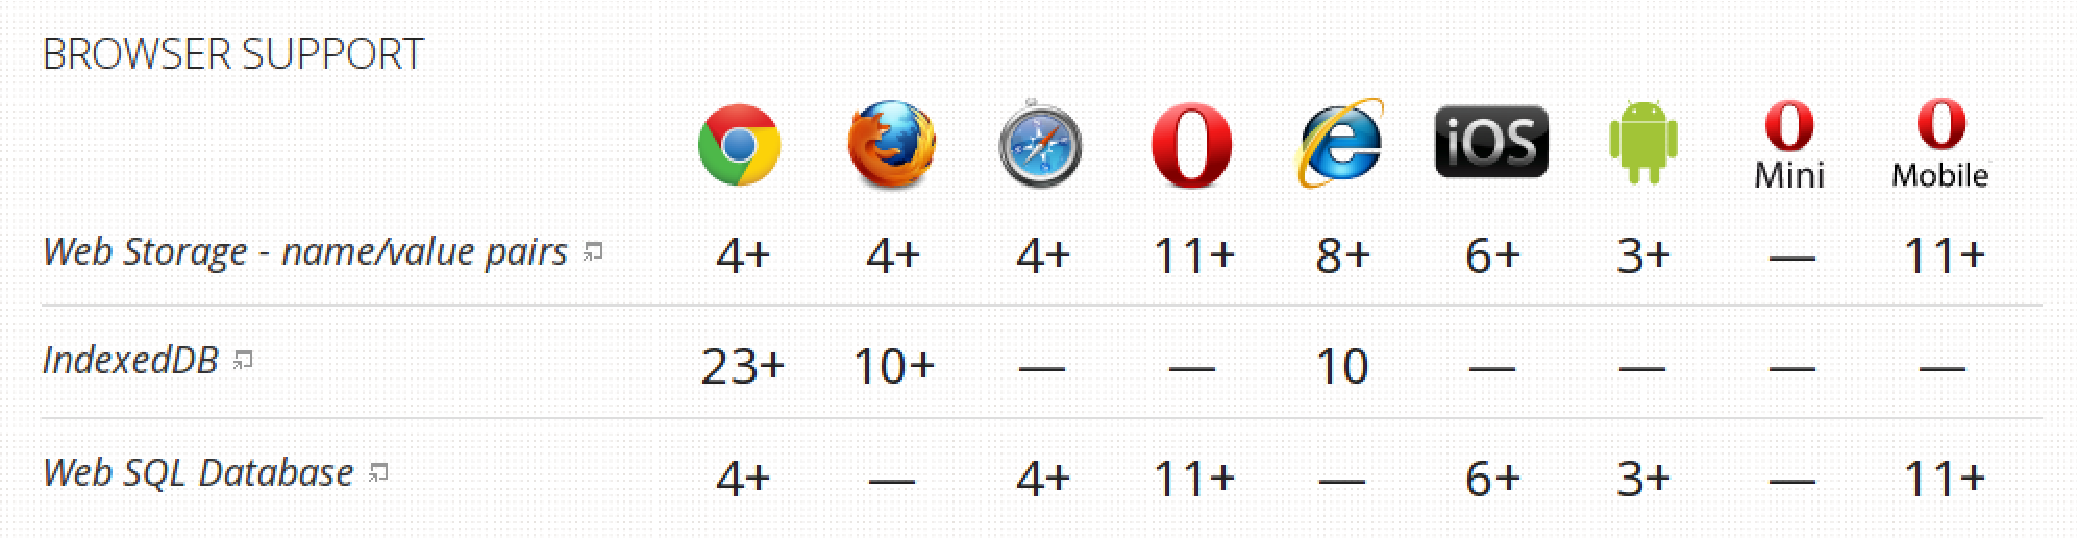
\includegraphics[width=\textwidth,height=\textheight,keepaspectratio]{./Figures/storage_browser_compatibility.pdf}
    \rule{35em}{0.5pt}
  \caption[Storage Browser Kompatibilität]{Browser"=Kompatibilität der unterschiedlichen Storage"=Technologien}
  \label{fig:storage_browser_compatibility}
\end{figure}
Abbildung \ref{fig:storage_browser_compatibility} zeigt, welche der vorgestellten Techologien aktuell in welchen Browsern unterstützt werden. Wie man sieht, wird bisher nur der Web"=Storage flächendeckend und insbesondere auch in mobilen Browsern unterstützt. Vor allem Mozilla hat sich sehr stark gegen Web \ac{SQL} und für die Verwendung von IndexedDb ausgesprochen und unterstützt auch nur noch die letztere Technologie. Gegen diese Entscheidung gibt es aufgrund der im Gegensatz zu Web \ac{SQL} bedeutend komplexeren \ac{API} und der komplizierten Systementwicklung auf Basis von IndexedDb eine Menge Widerspruch (vgl. \cite{Ranganathan2010}). Momentan sieht es aber danach aus, dass IndexedDb zu einer \ac{W3C}"=Empfehlung wird, während Web \ac{SQL} nur von einzelnen Browserherstellern unterstützt wird.

Anforderung \reqref{requirementOfflineWork} fordert, dass der Anwender zumindest rudimentär mit dem System arbeiten kann, auch wenn keine Verbindung zu dem Backend besteht. Hierfür ist es notwendig, dass vom Anwender erstellte Daten und Änderungen im Browser vorgehalten werden, damit sie bei einer Wiederherstellung der Konnektivität synchronisiert werden können. Für die Umsetzung dieser Anforderung wurde in dieser Arbeit eine Entscheidung für den Web"=Storage und gegen Web"=\ac{SQL} und die IndexedDb"=\ac{API} getroffen. Ein Grund dafür ist, dass der Web"=Storage, wie in Abbildung \ref{fig:storage_browser_compatibility} deutlich wird, momentan die größte Verbreitung in aktuellen und insbesondere mobilen Browsern genießt. Insbesondere für Web"=\ac{SQL} ist hier in Zukunft auch keine Verbesserung zu erwarten. Des Weiteren ist die Erstellung einer Applikation auf IndexedDb"= und Web"=\ac{SQL}"=Basis deutlich komplexer als auf Basis von Web"=Storage, welcher für das einfache Hinterlegen von zu synchronisierenden Daten ausreicht. Durch seine einfachen Schlüssel"=/Wertpaare ist er in der Umsetzung und Pflege bedeutet einfacher zu Handhaben als die anderen beiden Systeme. In Bezug auf IndexedDb ist es außerdem problematisch, dass sich die \ac{API} noch nicht in einem finalisiertem Zustand befindet und noch größere Änderungen mit neuen Browserversionen zu erwarten sind.

\subsection{Online-/Offline-Erkennung}\label{section:online_offline_erkennung}
Anforderung \reqref{requirementCheckOnlineStatus} fordert, dass das System seinen Onlinestatus kennen und bemerken muss, wenn sich dieser ändert. In aktuellen Browsern existiert eine \ac{API}, die es dem System erlaubt zu erkennen, ob eine Verbindung mit dem Internet besteht oder nicht. Zum einen gibt es die Eigenschaft \texttt{onLine} des globalen \texttt{navigator}"=Objektes. \texttt{navigator.onLine} is \texttt{true}, wenn eine Netzwerkverbindung besteht und ansonsten \texttt{false}. Zum anderen wird bei Änderung des Online"=/Offline"=Zustandes ein Event ausgelöst, für welches im Code Listener definiert werden können:
\begin{lstlisting}
document.body.addEventListener("online", function () {...} 
document.body.addEventListener("offline", function () {...}.
\end{lstlisting}          
Diese in den Listenern definierten Callbacks werden bei einem Wechsel von online zu offline oder umgekehrt ausgeführt. Es ist jedoch zu beachten, dass unterschiedliche Browserhersteller "`offline"' unterschiedlich definieren. Aktuell wechselt zum Beispiel Chrome bei Verlust der Internetverbindung in den Offline"=Modus, im Firefox muss dieser Modus explizit vom User angeschaltet werden (vgl. \cite{MozBug2011}).

\section{Kommunikation in Mashup-Anwendungen}\label{section:kommunikation_in_mashup_anwendungen}
Die Anforderungen \reqref{requirementAggregator} und \reqref{requirementUsageInBrowser} verlangen, dass das System einen Aggregator, also eine Mashup"=Anwendung (siehe Abschnitt \ref{section:mashup_anwendungen}) darstellt, der unterschiedliche Systeme in aktuellen Browsern zusammenfasst. Des Weiteren soll der Nutzer in einer Art Dashboard Informationen über den Zustand der einzelnen Widgets erhalten (\reqref{requirementDashboard}). Dies erfordert, dass die Widgets in der Lage sind mit der Hauptapplikation zu kommunizieren. Die Widgets werden, wie in Abschnitt \ref{section:widget_frameworks} beschrieben, von einer Wookie"=Instanz, also von einem anderen Server als die Hauptapplikation ausgeliefert. Zusammengenommen zieht dies Probleme mit den Sicherheitsrichtlinien innerhalb der Browser nach sich. Dieses Kapitel behandelt diese sogenannte Same"=Origin"=Policy und stellt Lösungswege vor, wie trotz der gegebenen Einschränkungen eine Mashup"=Anwendung funktionieren kann.

In einer Mashup"=Anwendung müssen mehrere System miteinander kommunizieren. Auch und insbesondere im Hinblick auf eine einfache Erweiterbarkeit (Anforderung \reqref{requirementExtensibility}) ist es von Vorteil, wenn die Bestandteile der Anwendung für ihre Anfragen einen ähnliches Prinzip verwenden. Bei der Verwendung eines gemeinsamen Interfaces würde sich die Interoperabilität zwischen den Teilanwendungen erhöhen Entwicklern das Hinzufügen neuer Anwendungen zu der Anwendung beträchtlich erleichtern. In den letzten Jahren ist hierfür das REST"=Prinzip immer weiter in den Fokus gerückt, welches ebenfalls in diesem Kapitel vorgestellt wird.

\subsection{Same-Origin-Policy}\label{section:same_origin_policy}
Moderne Browser benutzen als Teil ihres Sicherheitskonzeptes die Same"=Origin"=Policy. Diese bewirkt, dass Sprachen, die auf Client"=Seite ausgeführt werden (wie Javascript), nicht die Möglichkeit haben, Requests, also Anfragen, an einen anderen Zielpunkt als ihrem Ursprung zu starten (vgl. \cite{Ruderman2008}). Diese Policy wird also lediglich bei Zugriff auf \acp{URL} mit der selben Domain und dem selben Port, wie die \ac{URL} von der die Seite geladen wurde, erfüllt. Das bedeutet, dass ein Skript auf \path{http://sop.example.com/directory1} Requests an \path{http://sop.example.com/directory2} starten kann, nicht jedoch an \path{http://example.com/directory2} (unterschiedliche Domain) oder an \path{http://sop.example.com:8080/directory2} (unterschiedlicher Port). Ausgenommen ist hierbei das in eine Seite eingebettete Laden von Ressourcen. Hierzu gehören externe Inhalte, die über iframes geladen werden aber auch externe Javascript"=Dateien (über $<$script$>$...$<$/script$>$ Tags) und Medienressourcen wie Bilder und Videos. Des Weiteren ist es auch möglich Formulare an andere Zielpunkte als den Ursprung abzuschicken. Diese Einschränkung hat also primär Auswirkungen auf das Absenden von XMLHttp"=Requests, also auf normale Ajax"=Requests.

Die Same"=Origin"=Policy ist sehr sinnvoll, um beispielsweise gefährlichem Javascript"=Code das Ausspähen privater Daten zu verhindern. Sie erschwert jedoch die Entwicklung moderner Ajax"=Anwendungen und insbesondere die Entwicklung von Mashup"=Applikationen wie \acp{PLE}, welche prinzipiell so aufgebaut sind, dass sie ihre Inhalte und Ressourcen aus unterschiedlichen Quellen beziehen. In einer \ac{PLE} wie in dieser Arbeit beschrieben, werden die Widgets von einem Widget"=Container wie Wookie (siehe Abschnitt \ref{section:widget_frameworks}) ausgeliefert und besitzen dadurch auch die Domain des Widget Containers als Origin. Arbeiten diese Widgets nun aber nicht nur lokal beim Client, sondern benötigen für ihre Funktionalität auch externe Server, so müssen sie in der Lage sein XMLHttp"=Requests an diese zu senden. Aus diesem Grund wurde der Mechanismus des \ac{CORS} (vgl. \cite{vanKesteren2012}) eingeführt. Dieser erlaubt es unter bestimmten Bedingungen und Einschränkungen die Same"=Origin"=Policy zum umgehen.

\subsubsection*{\ac{CORS}}
Wenn \acl{CORS} benutzt wird, kann der Server so konfiguriert werden, dass er Anfragen von anderen Origins erlaubt und angibt welche Header in diesen Anfragen vorkommen dürfen. Ein einfacher \ac{CORS}"=Request vom Client zum Server sieht wie folgt aus (Workflow analog zu \cite{Hossain2012}):
Der Client sendet eine Cross"=Origin"=Anfrage mit einem Origin Header an den Server:
\begin{lstlisting}
GET /cors HTTP/1.1
Origin: http://api.bob.com
Host: api.alice.com
\end{lstlisting}
Anschließend antwortet der Server mit:
\begin{lstlisting}
Access-Control-Allow-Origin: http://api.bob.com
Access-Control-Allow-Credentials: true
Access-Control-Expose-Headers: FooBar
\end{lstlisting}
Alle für den \ac{CORS}"=Request relevanten Header beginnen mit Access"=Control.\\ \texttt{Access\allowbreak -Control\allowbreak -Allow\allowbreak -Origin} bedeutet, dass der Server eine Cross"=Origin"=Anfrage von dem angegebenen Origin erlaubt, \texttt{Access\allowbreak -Control\allowbreak -Allow\allowbreak -Credentials: true} besagt, dass in diesem Request auch Cookies erlaubt sind. Möchte der Client Zugriff auf Nicht"=Standard"=Header aus der Antwort des Servers, müssen diese in \texttt{Access\allowbreak -Control\allowbreak -Expose\allowbreak -Headers} angegeben werden.

Sollte der Client einen Request mit einer anderen Methode als \texttt{GET} oder \texttt{POST} (siehe Abschnitt \ref{section:rest}) senden, reicht dieser einfache Workflow nicht aus. In diesem Fall muss vor der eigentlichen Anfrage ein so genannter "`Preflight"=Request"' ablaufen, welcher verifiziert, dass der Server diese Methode als \ac{CORS}"=Request erlaubt.

Diese Methodik erlaubt also, das Widgets von einem Widget"=Container ausgeliefert werden, dadurch einen anderen Origin bekommen und trotzdem Requests an ihr eigentliches Backend senden zu können. Damit ist sie ein essentieller Baustein für den Aufbau von Mashup"=Anwendungen im Internet.

\subsubsection*{Postmessage}
Für die in Anforderung \reqref{requirementWidgetInformSystem} geforderte Darstellung der wichtigsten Informationen über den Zustand eines Widgets ist es notwendig, dass die Hauptapplikation Daten von den Widgets erhalten oder auslesen kann. Mashup"=Anwendungen im Internet werden, wie in Kapitel \ref{section:widgets} beschrieben, hauptsächlich über iframes umgesetzt. Die Same"=Origin"=Policy aktueller Browser erlaubt aber nur, dass die Hauptanwendung lediglich Daten aus iframes mit der gleichen Origin ausliest. Dies erschwert den Informationsaustausch zwischen der Hauptapplikation und den Widgets beträchtlich. Aus diesem Grund wurde das "`Postmessage"' System entwickelt, welches diese Einschränkung auf eine sichere Art und Weise umgeht. Mit Hilfe von Postmessage ist es möglich, dass sich unterschiedliche Fenster (zum Beispiel Frames) Nachrichten schicken können. Andere Fenster können Event"=Listener implementieren, welche auf diese Nachrichten hören (vgl. \cite{MDN2012}). Im folgenden Listing wird deutlich, wie solch eine Nachricht versendet wird (aus \cite{MDN2012}):
\begin{lstlisting}
otherWindow.postMessage(message, targetOrigin);
\end{lstlisting}
\texttt{otherWindow} ist hierbei eine Referenz auf ein anderes Fenster oder einen anderen Frame, welches über einfache \ac{DOM}"=Methoden zu erreichen ist. \texttt{message} ist die Nachricht selber (kann auch ein Javascript"=Objekt sein) und \texttt{targetOrigin}, ist die Origin, die \texttt{otherWindow} haben muss, damit die Nachricht verschickt wird. Damit \texttt{otherWindow} die Nachricht empfängt, muss auf dieser Seite ein Event Listener implementiert werden:
\begin{lstlisting}
window.addEventListener("message", receiveMessage);
function receiveMessage(event) {
  if (event.origin !== "http://example.org:8080")
    return;
  // ...
\end{lstlisting}
Empfängt das Fenster also eine Nachricht ist es möglich auch den Origin des Senders zu prüfen, damit man nur Nachrichten aus vertrauenswürdigen Quellen bearbeitet.

Mit dieser Technik ist es möglich, dass sich Widgets bei der Hauptapplikation registrieren und ihr Informationen, z.B. über die Anzahl der vorhandenen Einträge, zukommen lassen. Diese Informationen kann die Hauptapplikation dann für den Anwender aufbereiten und darstellen, so dass sich Anforderung \reqref{requirementWidgetInformSystem} erfüllen lässt.

\subsection{\acs{REST}}\label{section:rest}
\ac{REST}, ist ein Architekturstil, welcher versucht 
\begin{quotation}
[...] für statische Inhalte und dynamisch berechnete Informationen, die ein globales, gigantisches Informationssystem bilden, ein einheitliches Konzept zu definieren (\cite{tilkovrest}, Seite 10).
\end{quotation}
Wird ein System nach dem \ac{REST}-Prinzipien entworfen, führt dies im Idealfall zu positiven Eigenschaften, wie der losen Kopplung von Systemen, dem Vorhandensein allgemeiner Interfaces und einer dadurch erhöhten Interoperabilität, Wiederverwendbarkeit und Erweiterbarkeit (vgl. \cite {tilkovrest}).

Theoretisch ist es möglich ein beliebiges \ac{REST}"=konformes Protokoll zu entwickeln und anzuwenden, normalerweise wird jedoch das im Internet dominierende \ac{HTTP}"=Protokoll für die Umsetzung benutzt. Der Grund hierfür ist, dass dieses Protokoll bei korrekter Anwendung die wichtigsten Anforderungen des \ac{REST}"=Prinzips erfüllt und schon im Hinblick auf diesen Architekturstil entworfen wurde (einer der Hauptbeteiligten am Entwurf der \ac{HTTP}"=Spezifikation, Roy Fielding, hat mit seiner Dissertation :"`Architectural Styles and the Design of Network"=based Software Architectures"' das \ac{REST}"=Prinzip entwickelt (vgl. \cite{Fielding2000})). 
In einem \ac{REST}"=Entwurf wird nach Entitäten gesucht, welche auf Ressourcen abgebildet werden. Dies ähnelt einem objektorientierten Entwurf, es gibt hierbei jedoch zwei wichtige Unterschiede. Es werden den Ressourcen keine neuen Methoden oder Verben hinzugefügt, sondern es werden nur die Standardmethoden genutzt. Um trotzdem keine Einschränkung in der Mächtigkeit dieses Prinzips in Kauf nehmen zu müssen, werden mehr Ressourcen hinzugefügt, als es eigentlich Entitäten gibt. In einem dem \ac{REST}"=Prinzipien folgenden System speichert der Server keinerlei Session Informationen über den Nutzer. Dies hat zur Folge, dass beispielsweise der Warenkorb in einem Shop ebenfalls als Ressource angelegt werden muss. Der Vorteil von dieser Vorgehensweise ist der, dass somit z.B. auch Lesezeichen auf einen Warenkorb angelegt werden können. Zusätzlich gibt es beispielsweise noch neben den Primärressourcen, welche einzelnen Entitäten abbilden, Listenressourcen welche für die Auflistung einer Menge von Ressourcen eines bestimmten Typen genutzt werden (vgl. \cite{tilkovrest}). Im Internet besteht bereits ein eindeutiges System für die öffentliche Vergabe von Ressourcen"=Identifizierern: die \ac{URI}, z.B. \path{http://example.com/accounts/5?paginate=1&page=3}). URIs stellen einen allgemein verfügbaren Namensraum zur Verfügung, in dem Ressourcen identifiziert werden können. \ac{REST} fordert, dass Ressourcen in unterschiedlichen Repräsentationen ausgeliefert werden können. So ist es beispielsweise möglich, dass es eine maschinenlesbare Repräsentation im \ac{XML}"=Format und eine für Menschen im Browser darstellbare Repräsentation im \ac{HTML} Format gibt. Der Client kann über einen Accept"=Header ein bestimmtes Format anfordern.
Möchte man zum Beispiel einen Kunden über eine Ressource abbilden könnte der Identifizierer \path{http://example.com/customers/4} sein. Eine Anfrage der Darstellung kann dann als einfacher \ac{HTTP}"=Request abgeschickt werden:
\begin{lstlisting}
GET /customers/4 HTTP/1.1
Host: example.com
Accept: application/xml 
\end{lstlisting}
Der Server gibt in mit einem Statuscode (hier 200 OK) zurück, ob die Anfrage erfolgreich war und fügt dann die gewünschte Repräsentation der Ressource an:.
\begin{lstlisting}
HTTP/1.1 200 OK
...
[XML spezifische Kopfzeilen]
<customer href="./customers/4">
  <name>Roman Sachse</name>
  <orders>
    <order>
      <delivered>true</delivered>
      <link>http://example.com/orders/54>
\end{lstlisting}
In der Antwort des Servers finden sich Links auf weitere mit dem Kunden verknüpfte Ressourcen. Dies ist eine Umsetzung des Hypermedia"=Prinzips, welches für ein vollkommenes \ac{REST}"=System fordert (vgl. \cite{tilkovrest}), dass sich der Client ab einem Startpunkt aus nur durch das Verfolgen von Links durch das gesamte System bewegen könnte. Eine Listenressource würde man über \path{http://example.com/customers} abfragen, die Antwort könnte dann in \ac{XML}"=Verweise auf die einzelnen Customer erhalten. Zusätzlich könnten bei gewünschter Paginierung der Ergebnisse (beispielsweise über Query"=Parameter wie \path{http://example.com/customers?page=2} noch Links auf die vorherige und nächste Seite zurückgegeben werden.

Wie man in der obigen Anfrage sieht, wird eine Anfrage mit dem Verb GET an den Server geschickt. Das \ac{HTTP}"=Protokoll stellt unterschiedliche Standardmethoden bereit, mit denen ein Client eine Ressource abfragen kann. Der Vorteil bei der Nutzung dieser Standardmethoden liegt darin begründet, dass mit ihnen ein Interface existiert, mit dem alle Ressourcen abgefragt werden können und die ein Server für alle Ressourcen versteht. Sollte dies einmal nicht der Fall sein, kann der Server mit einer Fehlermeldung im Sinne von "`Methode wird für diese Ressource nicht unterstützt"' antworten. \ac{HTTP} stellt acht Methoden bereit, wobei hier aus Gründen des Umfangs nur die in der Praxis wichtigsten und auch in der Arbeit verwendeten fünf kurz vorgestellt werden (vgl. \cite{tilkovrest}):
\begin{enumerate}
 \item mit \texttt{GET} fordert der Client eine Repräsentation einer Ressource an.
 \item \texttt{PUT} aktualisiert oder erstellt (wenn nicht vorhanden) eine Ressource. 
 \item \texttt{POST} erstellt eine Ressource (wird an Listenressource gesendet).
 \item \texttt{DELETE} löscht eine Ressource.
 \item \texttt{OPTIONS} liefert Metadaten für eine Ressource - z.B. Allow"=Header, welche angeben, welche Methoden/Header akzeptiert werden (siehe Abschnitt \ref{section:same_origin_policy}).
\end{enumerate}

Um zu den Customer"=Ressourcen aus dem obigen Beispiel also einen Kunden hinzuzufügen, müsste man einen POST"=Request an die Listenressource \path{http.example.com/customers} senden. Ein einzelner Kunde kann mit einem GET"=Request an die Primärressource \path{http.example.com/customers/4} ausgelesen werden. PUT oder DELETE würden die Ressource dementsprechend aktualisieren oder löschen

GET und POST sind die am häufigsten genutzten Methoden. Der Grund hierfür ist, dass diese beiden Methoden der normale Weg eines Browser sind mit einem Server zu kommunizieren. Jeder direkte Aufruf einer URI über einen Browser sendet eine GET"=Anfrage an einen Server. Die im Web häufig anzutreffenden Formulare werden meist über eine POST"=Anfrage abgeschickt. So werden diese beiden Methoden ausserhalb von Anwendungen, die dem \ac{REST}"=Prinzip folgen, auch für alle anderen Anfragen benutzt, so dass man sich bei diesen Anwendungen nicht sicher sein kann, ob ein GET"=Request an eine URI nicht ein Ändern oder Löschen der Ressource zur Folge hat (man betrachte beispielsweise die URI: \path{http://example.com/customers/5?action=delete}).

Wird eine Anwendung im Hinblick auf \ac{REST}"=Prinzipien umgesetzt, so vereinfacht dies die Erweiterung dieses Systems beträchtlich (Anforderung \reqref{requirementExtensibility}). Insbesondere für Mashup"=Anwendungen bei denen unterschiedliche Systeme miteinander kommunizieren müssen, ist beispielsweise die Nutzung eines gemeinsamen Methodeninterfaces sehr hilfreich, da nicht für jedes System ein weiteres Kommunikationsprotokoll erstellt werden muss. Das System dieser Arbeit hat noch die zusätzliche Anforderung den Anwender in die Lage zu versetzen auch offline zu arbeiten (Anforderung \reqref{requirementOfflineWork}). Wenn das System für das Speichern der Daten im Browser ebenfalls auf \ac{REST} aufsetzt, wird es mit relativ wenig Aufwand möglich sein weitere offline fähige Widgets für unterschiedliche Services zu erstellen. Die Art des Services ist dabei egal, solange er in der Lage ist einfache \ac{REST}"=Anfragen zu verstehen, zu verarbeiten und standardkonform auf sie zu antworten. Für den Entwickler wird es in diesem Fall vollkommen transparent sein, ob sich das System in einem online oder offline ist. Er kann unabhängig von dem Zustand die Daten ohne zu implementierende Fallunterscheidungen speichern und abfragen.

\section{Eine \ac{PLE} auf dem USB-Stick}\label{section:ple_auf_usb}
Anforderung \reqref{requirementUsbStick} fordert die Möglichkeit das System auf unterschiedlichen Rechnern zu benutzen und die Daten offline zwischen diesen Rechnern auszutauschen. Da alle systemrelevanten Daten im Browser hinterlegt werden (Application"=Cache (siehe Abschnitt \ref{section:appcache}) und Web"=Storage (siehe Abschnitt \ref{section:offline_storage}), ist es notwendig die gesamte Browserinstallation zwischen unterschiedlichen Rechnern hin und herbewegen zu können. Der einfachste Weg hierfür ist die Installation des Browsers auf einem portablen Speichermedium wie einem USB"=Stick. Hierfür gibt es beispielsweise die Open"=Source"=Anwendung \href{http://portableapps.com/}{PortableApps}\footnote{weitere Informationen auf: \url{http://portableapps.com/}}, die genau dies erlaubt. Leider existieren solche Möglichkeiten bisher nur auf Windows-Systemen, so dass diese Anforderung nicht auf anderen Betriebssystemen wie zum Beispiel Distributionen auf Linux Basis zu erfüllen ist.  % Übersicht Stand der Forschung

\chapter{Konzeptuelle Lösung - Plesynd} 
\label{chapter:Kapitel5}
\lhead{Kapitel 5 \emph{Konzeptuelle Lösung - Plesynd}}  
Das Ziel dieser Arbeit ist der Entwurf und die prototypische Implementierung einer leichtgewichtigen Personal Learning Environment mit Offline"=Funktionalitäten auf Basis aktueller Technologien, welche die Anforderungen aus Kapitel \ref{chapter:Kapitel3} erfüllt. 

Der Name des entwickelten Systems lautet \emph{Plesynd} (Personal Learning Environment Synchronize Data) und wird wie das englische "`pleasant"' (angenehm) ausgesprochen. Plesynd ist ein webbasiertes Dashboard, welches die Möglichkeit bietet mit unterschiedlichen Widgets in Kommunikation zu treten. Wichtig ist hierbei eine Abgrenzung zu zentralisierten Lern"=Management"=Systemen wie Moodle oder Sakai. Die sind sehr kurszentriert und entsprechen nicht dem nutzerzentrierten Ansatz von Personal Learning Environments. Aus diesem Grund orientiert sich Plesynd viel stärker an bestehenden Widget"=Aggregatoren wie iGoogle oder Netvibes (siehe Abschnitt \ref{section:aehnliche_systeme}). In einem nutzerzentrierten Ansatz, muss dem Anwender die Möglichkeit gegeben werden in unterschiedlichen Kontexten mit dem System zu arbeiten. Hierzu erlaubt es Plesynd dem Anwender seine Widgets in einer frei wählbaren Anzahl unterschiedlicher Bereiche, sogenannter Workspaces, aufzuteilen. Der entscheidende Unterschied von Plesynd zu den erwähnten Systemen ist die Offline"=Fähigkeit der PLE. Es wurde ein Ansatz entwickelt, der es ermöglicht das System auch ohne Internetverbindung zu starten und Widgets so zu implementieren, dass ihre Informationen offline verfügbar gemacht werden und offline mit Plesynd und den Widgets weitergearbeitet werden kann. Sobald der Browser wieder eine Online"=Verbindung hergestellt hat, werden die veränderten Daten mit dem Backend synchronisiert. Zusätzlich zu dem Grundsystem von Plesynd wurde in dieser Arbeit ein Todo"=Listen Widget entwickelt, welches die erwähnten Funktionalitäten nutzt und zeigt wie dem System zusätzliche Widgets hinzugefügt und komplett in Plesynd integriert werden können. Das komplette entwickelte System, inklusive der benötigten Komponenten, wurde der Arbeit als CD beigefügt. Eine Installationsanleitung befindet sich im Anhang.

Das vorliegende Kapitel liefert einen Überblick über die grundsätzliche Architektur von Plesynd und seiner Komponenten und eine Beschreibung des implementierten User"=Interfaces.

% \begin{landscape}
\begin{figure}
  \centering
  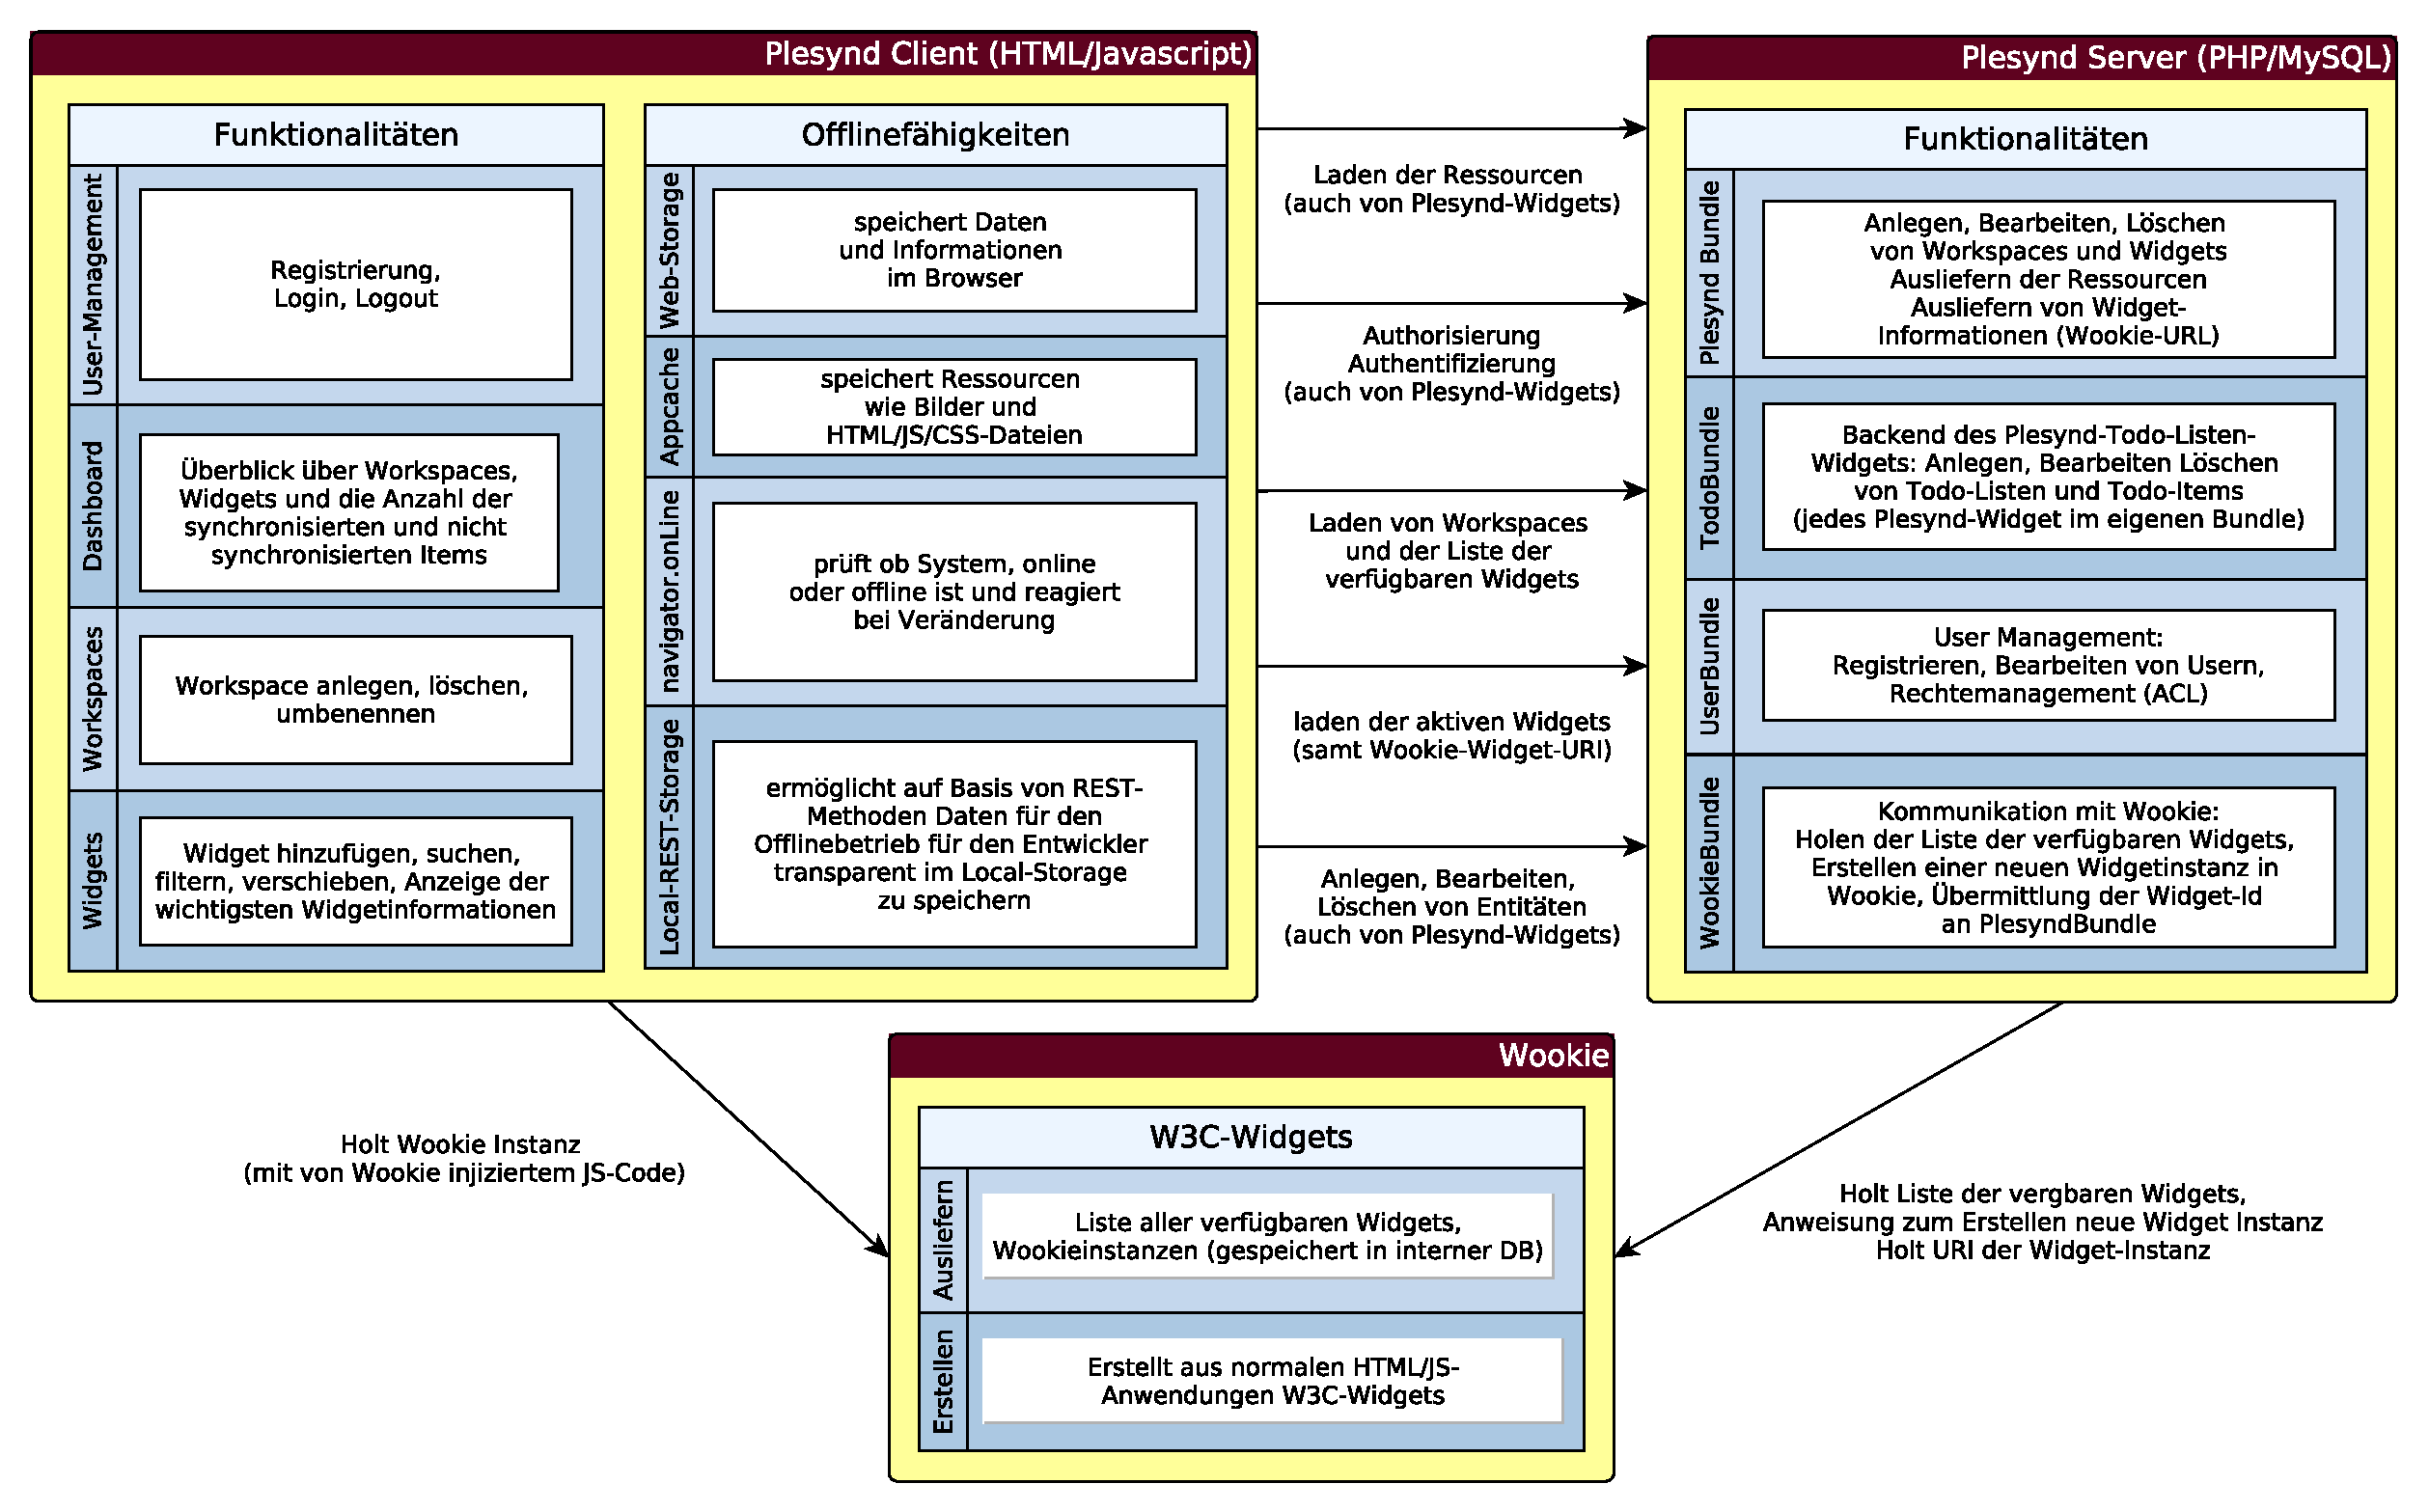
\includegraphics[width=\textwidth,keepaspectratio]{./Figures/konzeptionelle_loesung_table.pdf}
    \rule{35em}{0.5pt}
  \caption[Überblick über die Komponenten von Plesynd]{Überblick über die Komponenten von Plesynd}
  \label{fig:ueberblick_plesynd_komponenten}
\end{figure}
% \end{landscape}

\section{Überblick über die Architektur von Plesynd}\label{section:plesynd_architektur}
Zunächst gibt Abbildung \ref{fig:ueberblick_plesynd_komponenten} einen Überblick über die wichtigsten Komponenten des entwickelten Systems und über deren Zusammenspiel. Plesynd selbst besteht aus zwei Komponenten, Plesynd"=Client und Plesynd"=Server. Diese liefern zusammen die Funktionalitäten, welche die gestellten Anforderungen erfüllen sollen. Zusätzlich wird Wookie als externe Komponente zum Ausliefern und Erstellen der Widgets verwendet.

\subsection{Plesynd-Client}
\begin{figure}
  \centering
  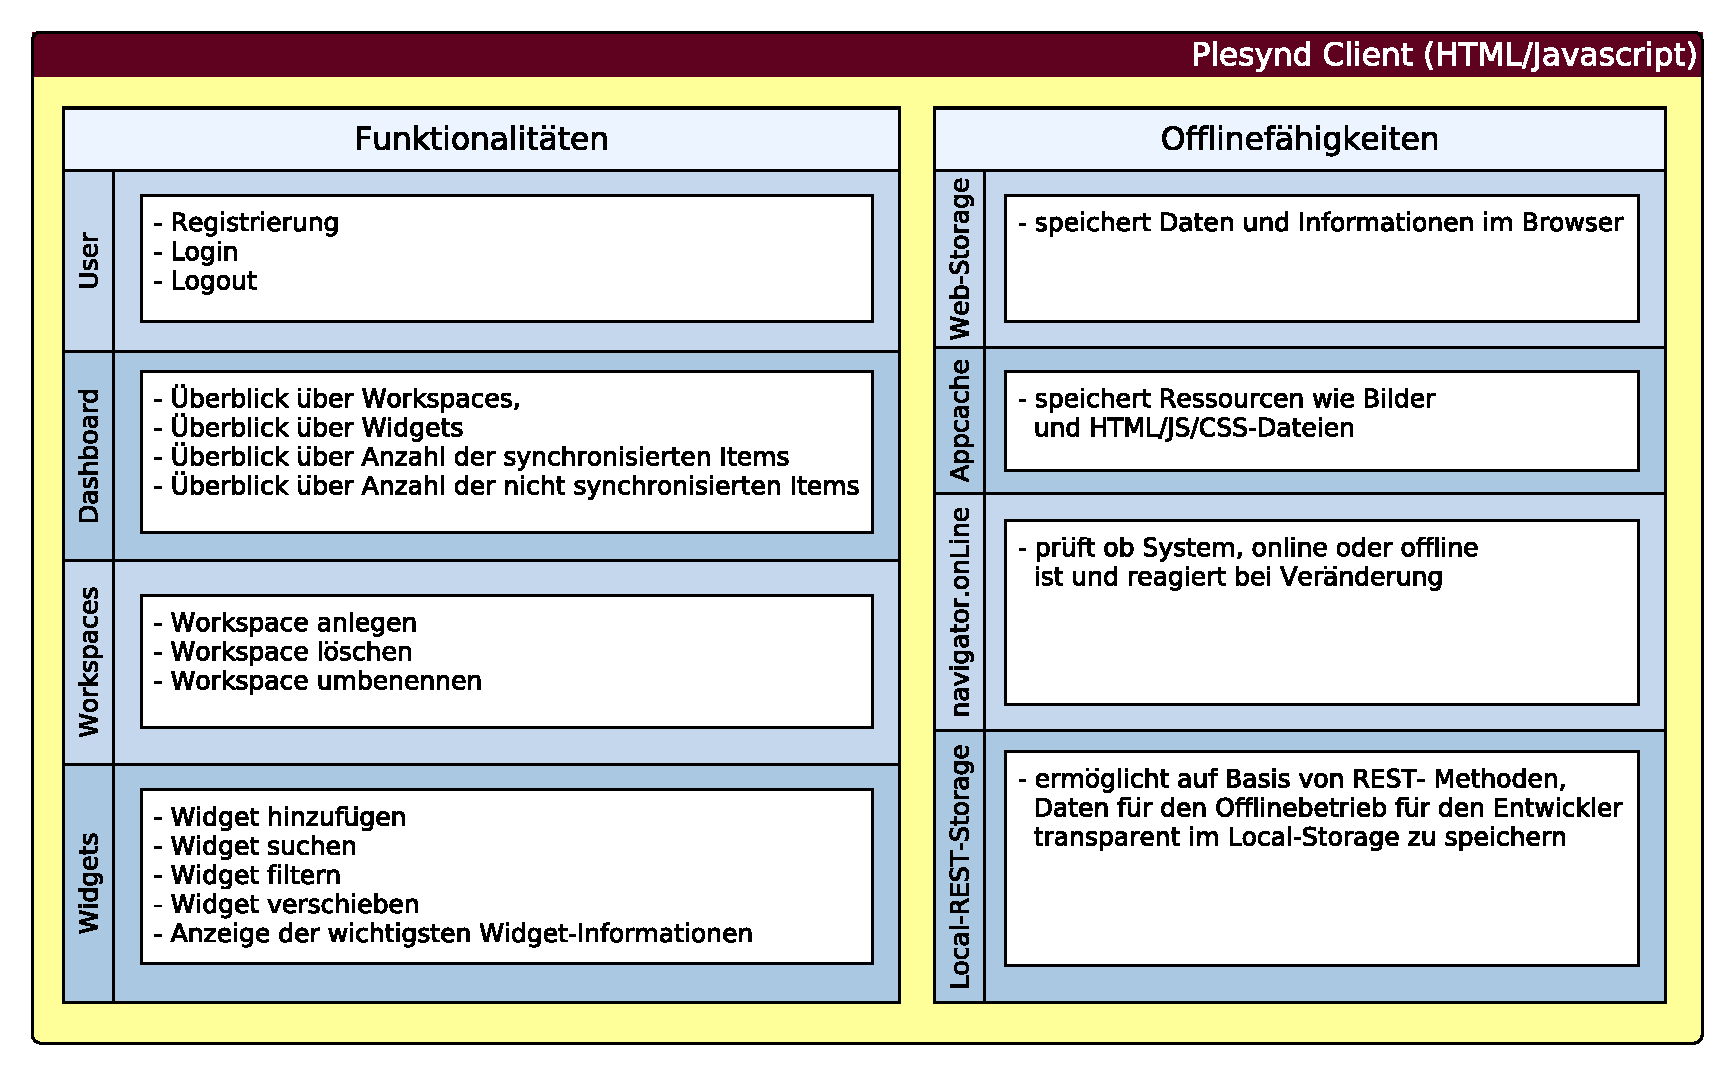
\includegraphics[height=10cm,keepaspectratio]{./Figures/konzeptionelle_loesung_plesynd_client.pdf}
    \rule{35em}{0.5pt}
  \caption[Überblick Plesynd-Client]{Überblick Plesynd-Client}
  \label{fig:ueberblick_plesynd_client}
\end{figure}
Plesynd"=Client (siehe Abbildung \ref{fig:ueberblick_plesynd_client}) bezeichnet den Teil der Anwendung, der direkt beim Client, also im Browser des Anwenders läuft. Diese Komponente umfasst den größten Teil des entwickelten Systems und ist auch für die Offline"=Funktionalitäten von Plesynd verantwortlich. Plesynd"=Client stellt über ein User"=Interface den Teil der PLE dar, mit dem der Anwender direkt in Berührung kommt. Es liefert Funktionalitäten zum Anlegen und Bearbeiten von Workspaces, versetzt den Anwender in die Lage nach Widgets zu filtern, diese den Workspaces hinzuzufügen und neu anzuordnen und stellt ihm ein Dashboard zur Verfügung auf dem die wichtigsten Informationen zu seinen Workspaces und Widgets zusammengefasst werden. Es informiert den Nutzer auch darüber, ob das System eine Verbindung zu dem Internet hat oder nicht. Zusätzlich gibt es dem Anwender die Möglichkeit sich zu registrieren und sich in das System einzuloggen. 

Die Fähigkeit von Plesynd und des Todo"=Listen"=Widgets Anwendungsdaten offline vorzuhalten wurde auf Basis der Web"=Storage Technologie entwickelt (siehe Abschnitt \ref{section:offline_storage}). Plesynd erkennt über ein globales Javascript"=Event (siehe Abschnitt \ref{section:online_offline_erkennung}), wenn sich der Browser in einem Zustand befindet, in dem er keine Konnektivität mit dem Internet besitzt. Das System informiert den Anwender darüber, kann aber auch entscheiden, welche Funktionalitäten es dem Nutzer nur noch eingeschränkt zur Verfügung stellt. Nimmt der Anwender Änderungen an den Daten vor, werden diese in den Local"=Storage geschrieben. Sobald sich das System wieder mit dem Internet verbindet, erkennt Plesynd diese Zustandsänderung und synchronisiert die Daten mit den zugrunde liegenden Services. Sollte einmal eine andere Speichertechnik als der Web"=Storage benötigt werden, ist das System so implementiert, dass die Art der lokalen Speicherung losgelöst von der restlichen Anwendung umgestaltet werden kann. Entwickelt wurde diese Funktionalität mit besonderem Augenmerk auf die Implementierung zusätzlicher Widgets. Dies bedeutet, dass auf Basis der vorliegenden Implementierung mit relativ wenig Aufwand weitere Widgets für unterschiedliche Services erstellt werden können. Die Art des Services ist nicht von Belang. Er sollte nur in der Lage sein einfache REST"=Anfragen (siehe Abschnitt \ref{section:rest}) zu verstehen, zu verarbeiten und standardkonform auf sie zu antworten. Die Möglichkeit, Ressourcen wie Javascript, CSS und HTML Dateien im Browser zu speichern, wurde mit der HTML5 Appcache"=API umgesetzt (siehe Abschnitt \ref{section:appcache}). Probleme, mit der bei modernen Browser üblichen Same"=Origin"=Policy (siehe Abschnitt \ref{section:same_origin_policy}) für Requests, wurden mit dem Cross"=Origin Resource Sharing (CORS) Mechanismus und der Postmessage"=API gelöst. 

\subsection{Plesynd-Server}
\begin{figure}
  \centering
  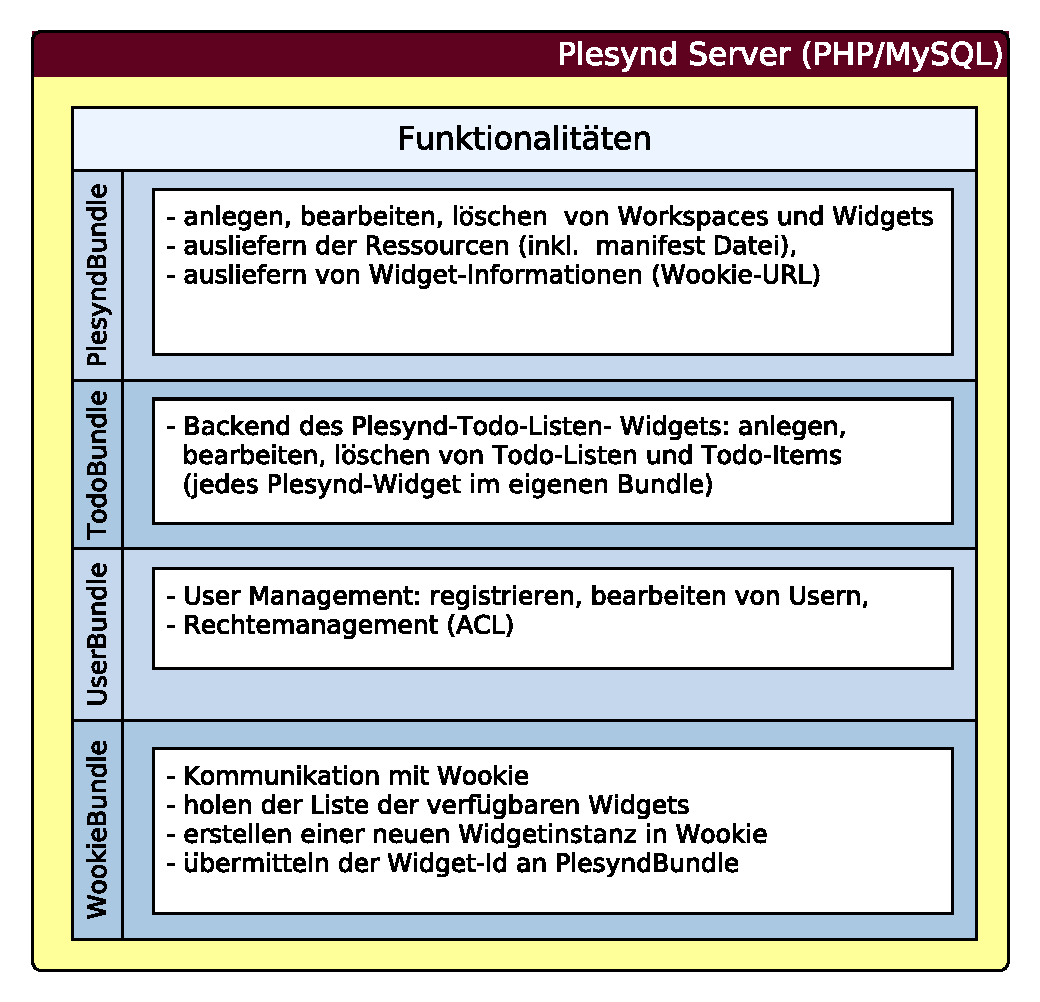
\includegraphics[height=10cm,keepaspectratio]{./Figures/konzeptionelle_loesung_plesynd_server.pdf}
    \rule{35em}{0.5pt}
  \caption[Überblick Plesynd-Server]{Überblick Plesynd-Server}
  \label{fig:ueberblick_plesynd_server}
\end{figure}
Plesynd"=Client ist, wie eben beschrieben, in der Lage sowohl Ressourcen als auch Daten lokal beim Client zu speichern und so auch offline verfügbar zu machen. Es benötigt zum normalen Betrieb aber ein Backend, welches diese Ressourcen initial ausliefert und sich um die persistente Speicherung der Daten und das Rechtemanagement kümmert. Für diesen Zweck wurde die Plesynd"=Server Komponente (siehe Abbildung \ref{fig:ueberblick_plesynd_server}) entworfen. Diese Komponente besteht aus mehreren Bundles (siehe Abschnitt \ref{section:symfony2}), wobei jedes Bundle für einen bestimmten Aufgabenbereich innerhalb  von Plesynd"=Server zuständig ist. Aufgaben von Plesynd"=Server sind das Ausliefern der Ressourcen, die Speicherung von Workspace und den zugehörigen Widgets samt ihrer Position auf dem Workspaces, das User"=Management (Registrierung, Login etc) und das Rechtemanagement, also die Prüfung welcher Nutzer Zugriff auf welchen Workspace, Widget oder welche Todo"=Liste hat. 

Plesynd"=Server nimmt für die Arbeit mit den Anwendungsdaten (Workspace, Widgets, Todo"=Listen etc.) REST konforme Anfragen (siehe Abschnitt \ref{section:rest}) entgegen und antwortet standardkonform.

Für die Abfrage welche Widgets grundsätzlich im System vorhanden sind verwendet Plesynd"=Server eine Schnittstelle zur Wookie"=Komponente. Diese Schnittstelle wird auch verwendet wenn der Anwender ein neues Widget zu einem Workspace hinzufügen möchten, also eine neue Widget"=Instanz erstellt werden muss.

\subsection{Wookie}\label{section:loesung_wookie}
\begin{figure}[ht]
  \centering
  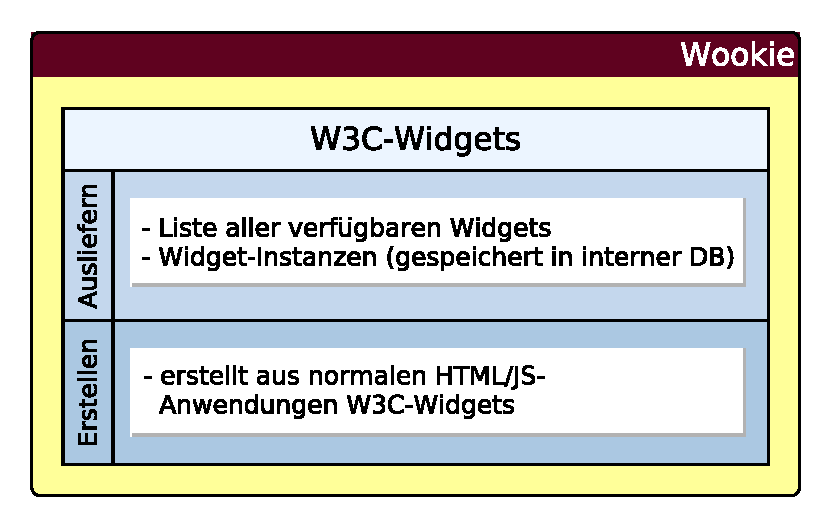
\includegraphics[height=5cm,keepaspectratio]{./Figures/konzeptionelle_loesung_wookie.pdf}
    \rule{35em}{0.5pt}
  \caption[Überblick Wookie]{Überblick Wookie}
  \label{fig:ueberblick_wookie}
\end{figure}
Als externe Komponente wird der W3C"=Widget"=Container Wookie (siehe Abbildung \ref{fig:ueberblick_wookie} und Abschnitt \ref{section:widget_frameworks}) eingebunden. Dieser speichert die verfügbaren Widgets in einer internen Datenbank und kann Plesynd so eine Liste der auslieferbaren Widgets zur Verfügung stellen. Wookie hinterlegt außerdem jede einzelne erstellte Widget"=Instanz samt ihrem Zustand und kann so das eigentliche Widget bei Bedarf an Plesynd"=Client ausliefern. Diese Funktionalität ist die einzige, bei der Plesynd"=Client direkt Kontakt zu Wookie aufnimmt, ansonsten wird die gesamte Kommunikation über Plesynd"=Server abgewickelt. Zusätzlich zu diesen Anwendungsfällen bietet Wookie Werkzeuge an, um aus normalen HTML/Javascript"=Applikationen ein W3C"=Widget zu erstellen. Diese Funktionalität steht jedoch nicht über die Kommunikation mit Plesynd zur Verfügung, sondern muss über die Kommandozeile in Anspruch genommen werden.

\section{Umsetzung}\label{section:umsetzung}

Die für die Umsetzung implementierten Funktionalitäten orientieren sich an den in Abschnitt \ref{section:anwendungsfaelle} definierten funktionalen Anforderungen. Für die Umsetzung der Screen"=Dimension (siehe Abschnitt \ref{section:dimensions_palmer}), also des User"=Interfaces kommen in Plesynd drei wichtige Konzepte zum Einsatz: Dashboard, Widgets und Workspaces. Über Widgets werden die unterschiedlichen Werkzeuge und Services, die ein Nutzer innerhalb des Systems nutzen möchte eingebunden (siehe Abschnitt \ref{section:widgets}). Die Umsetzung der einzelnen Widgets liegt in der Hand des jeweiligen Designers. Da Plesynd Wookie als Widget Container benutzt, ist es möglich alle W3C"=Widgets in das System einzubinden. Für diese Arbeit wurde ein Todo"=Listen"=Service entwickelt für den als prototypische Entwicklung ein Widget mit Online"=/Offline"=Fähigkeiten implementiert wurde. Besitzt ein Widget Online"=/Offline"=Fähigkeiten so erhält es eine von Plesynd zur Verfügung gestellte Statusleiste, in der der aktuelle Online"=/Offline"=Status sowie die Anzahl der verfügbaren Einträge und der noch nicht synchronisierten Einträge angezeigt wird (siehe Abbildungen \ref{fig:plesynd_workspace_online} und \ref{fig:plesynd_workspace_offline}). Der Nutzer hat die Möglichkeit Widgets nach Themen oder Einsatzgebieten zu gruppieren. Dies geschieht über sogenannte Workspaces. Workspaces sind vom Nutzer frei und in unbegrenzter Zahl hinzufügbare Bereiche im System. Sie sind über eine Reiter"=Navigation zu erreichen und können jederzeit umbenannt oder auch wieder gelöscht werden (siehe Abbildung \ref{fig:plesynd_workspace_edit}). Im folgenden werden die Umsetzungen der einzelnen Anforderungen genauer betrachtet.

Für die Umsetzung von Anforderung \reqref{requirementRegistrieren} (\emph{\requirementRegistrieren}) wurde eine Registrierungmechanismus implementiert. Ist der Anwender noch nicht registriert, hat er die Möglichkeit ein Anmeldeformular (siehe Abbildung \ref{fig:plesynd_register}) auszufüllen und dieses an den Server zu senden. Die gesendeten Daten werden validiert und führen im Fehlerfall zu einer erneuten Darstellung des Formulars samt Fehlermeldung und im Erfolgsfall zu einer Mitteilung an den Anwender, dass er sich als neuer Nutzer von Plesynd registriert hat. Abbildung \ref{fig:plesynd_register} zeigt ebenfalls die Umsetzung der Anforderung \reqref{requirementUniqueLoginEmail} (\emph{\requirementUniqueLoginEmail}). Zur Umsetzung von Anforderung \reqref{requirementLogin} (\emph{\requirementLogin}) hinterlegt Plesynd-Server die registrierten Anwender in einer Datenbank. Plesynd-Client bietet dem Nutzer die Möglichkeit sich über ein Formular an dem System anzumelden und anschließend mit ihm zu arbeiten (siehe Abbildung TODO).
Für Anforderung \reqref{requirementZugriffAufEigeneWidgets} (\emph{\requirementZugriffAufEigeneWidgets}) benutzt Plesynd, wie Abbildung \ref{fig:ueberblick_plesynd_server} zeigt, auf Serverseite Access-Control-Lists und hinterlegt damit für jeden Workspace und jedes Widget welcher Anwender diese erstellt und damit auch Zugriff auf sie hat. Andere Nutzer erhalten, auch wenn sie den Link zu einem Workspace kennen keinen Zugriff darauf. Ähnliches gilt ebenso für die mit Hilfe des Todo-Listen-Widgets erstellten Todo-Listen und Todo-Einträge. Klickt der Anwender auf den Link Logout (siehe Abbildung \ref{fig:plesynd_dashboard}), beendet das System seine Session und leitet ihn wieder auf die Login-Seite um. Dies stellt eine Umsetzung der in \reqref{requirementLogout} (\emph{\requirementLogout}) geforderten Funktionalität dar. Klickt der Anwender auf den Logout-Link, so wird seine Session auf dem Server beendet. Dies bedeutet, dass jeder weitere Request zu einem Fehler (403-Error) führt, welcher das System dazu veranlasst dem Anwender erneut die Login-Seite zu präsentieren. Es ist somit kein weiterer Zugriff auf die Daten möglich, was eine Realisierung von Anforderung \reqref{requirementKeinZugriffNachLogout} (\emph{\requirementKeinZugriffNachLogout}) darstellt. Zur Umsetzung von Anforderung \reqref{requirementWorkspaceAdd} (\emph{\requirementWorkspaceAdd}) wurde ein Hinzufügen Button in der Reiternavigation des Systems (siehe Abbildung \ref{fig:plesynd_dashboard}) implementiert, welcher direkt einen neuen Workspace zu dem System hinzugefügt.  \reqref{requirementWorkspaceEdit} (\emph{\requirementWorkspaceEdit}) fordert das Bearbeiten von Workspaces. Hierzu befindet sich in der genannten Reiternavigation neben einem aktiven Workspace ein Icon (siehe Abbildung \ref{fig:plesynd_workspace_edit}). Aktiviert der Anwender dieses, öffnet sich ein Bereich zum Bearbeiten des Workspaces. In diesem kann der Name direkt geändert werden. In dem Bereich zum Ändern des Workspace befindet sich auch ein Button zum Löschen desselben (siehe Abbildung \ref{fig:plesynd_workspace_edit}). Klickt der Anwender auf diesen, so wird ihm ein Rückfragefenster präsentiert. Bestätigt er hier das Löschen, wird der Workspace samt seiner Widgets aus dem System entfernt. Dies stellt eine Realisierung von Anforderung \reqref{requirementWorkspaceDelete} (\emph{\requirementWorkspaceDelete}) dar. \reqref{requirementWidgetAdd} (\emph{\requirementWidgetAdd}), \reqref{requirementWidgetFilterName} \emph{\requirementWidgetFilterName} und \reqref{requirementWidgetFilterOnline} \emph{\requirementWidgetFilterOnline} werden folgendermaßen realisiert: Im Bereich zum Bearbeiten eines Workspaces wird dem Anwender eine Maske zum Hinzufügen von Widgets angezeigt (siehe Abbildung \ref{fig:plesynd_workspace_edit}). Hier ist es ihm möglich ein Widget aus der Liste der zur Verfügung stehende Widgets auszuwählen. Wird ein Widget ausgewählt, werden dem Anwender die wichtigsten Informationen zu diesem Widget präsentiert. Bei Klick auf einen Button zum Hinzufügen wird das ausgewählte Widget an der nächste freien Position dem Workspace angehängt. Plesynd-Client bietet dem Anwender in der Maske zum Hinzufügen von Widgets einen eigenen Bereich an, in dem nach dem Namen des Widgets gesucht werden kann (siehe Abbildung \ref{fig:plesynd_workspace_edit}). Diese Suche findet nur auf dem Client statt, sendet also keine weiteren Anfragen an Plesynd-Server. Der Suchbereich, enthält neben dem Suchfeld noch einen Filter-Button, der es erlaubt nur offline-fähige Widgets anzuzeigen (siehe Abbildung \ref{fig:plesynd_workspace_edit}). Diese Filterung findet wie die Suche nur auf dem Client statt. Zum Löschen eines Widgets (Anforderung \reqref{requirementWidgetDelete} \emph{\requirementWidgetDelete}) kann der Anwender auf einen Button in der Widget-Statusleiste (siehe Abbildung \ref{fig:plesynd_workspace_edit}) oder auf dem Dashboard (siehe Abbildung \ref{fig:plesynd_dashboard}) klicken. Ihm wird anschließend wird ein Rückfragefenster präsentiert. Bestätigt er hier das Löschen, wird das Widget aus dem Workspace und damit auch aus dem System entfernt. Befindet sich der Anwender auf einem Workspace und hat dieser Workspace mehr als ein Widget, so ist der Anwender in der Lage mit einem Klick auf die Widget-Statusleiste die Widgets per Drag and Drop auf dem Workspace neu anzuordnen. Die neuen Positionen werden direkt an den Server weitergegeben und somit persistiert (siehe Abbildung TODO). Dies stellt eine Umsetzung der in \reqref{requirementWidgetSortDragNDrop} (\emph{\requirementWidgetSortDragNDrop}) Drag and Drop Funktionalität dar. Zur Umsetzung der Anforderungen \reqref{requirementWidgetInformSystem} (\emph{\requirementWidgetInformSystem}) und \reqref{requirementWidgetInformUser} (\emph{\requirementWidgetInformUser})  wurde folgendermaßen vorgegangen: Wenn der Anwender ein Plesynd-kompatibles Widget zu einem Workspace hinzufügt, meldet sich dieses bei Plesynd an und kann es über die Anzahl der verfügbaren und synchronisierten und nicht synchronisierten Einträge informieren (siehe Abbildung TODO). Diese Funktionalität wurde über die Postmessage-API implementiert (siehe Abschnitt \ref{section:kommunikation_in_mashup_anwendungen}). Als Startseite von Plesynd wurde ein Dashboard umgesetzt, welches die Workspaces samt ihrer Widgets auflistet (siehe Abbildung \ref{fig:plesynd_dashboard}). Für jedes Widget erhält der Anwender die Information, ob es Plesynd-kompatibel ist. Falls dem so ist, werden dem Anwender angezeigt wie viele Einträge vorhanden und wie viele synchronisiert und nicht synchronisiert sind. Zusätzlich kann der Anwender über das Dashboard Widgets entfernen und sich über Links direkt zu den gewünschten Workspaces bewegen. Dieses Dashboard dient zur Realisierung von Anforderung \reqref{requirementDashboard} (\emph{\requirementDashboard}).

Die Anforderungen \reqref{requirementCheckOnlineStatus} (\emph{\requirementCheckOnlineStatus}), \reqref{requirementOnlineStatusInformUser} (\emph{\requirementOnlineStatusInformUser}), \reqref{requirementOfflineStart} \emph{\requirementOfflineStart}, \reqref{requirementOfflineWork} (\emph{\requirementOfflineWork}) und \reqref{requirementOnlineSync} (\emph{\requirementOnlineSync}) beschreiben die erforderlichen offline Funktionalitäten des Systems. Plesynd nutzt die in Abschnitt \ref{section:online_offline_erkennung} beschriebene Online-/Offline-Erkennung für die Umsetzung von Anforderung ). Der aktuelle Status wird dem Nutzer direkt im System (siehe Abbildung \ref{fig:plesynd_dashboard}) und bei Plesynd-kompatiblen Widgets (siehe Abbildung \ref{fig:plesynd_workspace_offline}) angezeigt. Plesynd-Client speichert mit Hilfe der HTML-Appcache-API (siehe Abschnitt \ref{section:appcache}) die benötigten Ressourcen beim erstmaligen Systemstart im Browser. Ab diesem Zeitpunkt ist es möglich das System auch ohne Online-Verbindung zu laden. Abbildung TODO zeigt, wie die Workspace und Widgets im Local-Storage hinterlegt werden. Mit Hilfe der in Abschnitt \ref{section:offline_storage} beschriebenen Techniken und der entwickelten Systematik zum Speichern und Synchronisieren von Daten (siehe Abschnitt \ref{section:offline_faehigkeiten}), ist es möglich mit Plesynd-Client und den kompatiblen Widgets offline zu arbeiten. Das System synchronisiert die hinzugefügten, geänderten und gelöschten Einträge mit den jeweiligen Backends, wenn wieder eine Verbindung zum Internet hergestellt wurde.


\begin{figure}[hb]
  \centering
  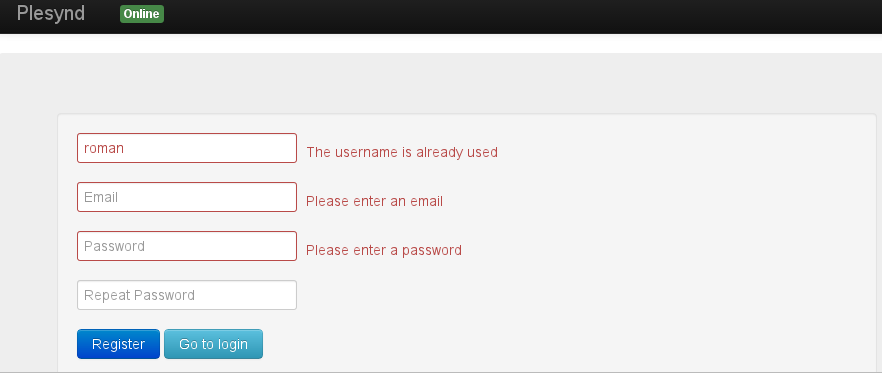
\includegraphics[]{./Figures/plesynd_register.png}
    \rule{35em}{0.5pt}
  \caption[Plesynd User"=Interface: Registrieren]{Der Anwender kann sich für die Nutzung von Plesynd registrieren}
  \label{fig:plesynd_register}
\end{figure}

\begin{figure}
  \centering
  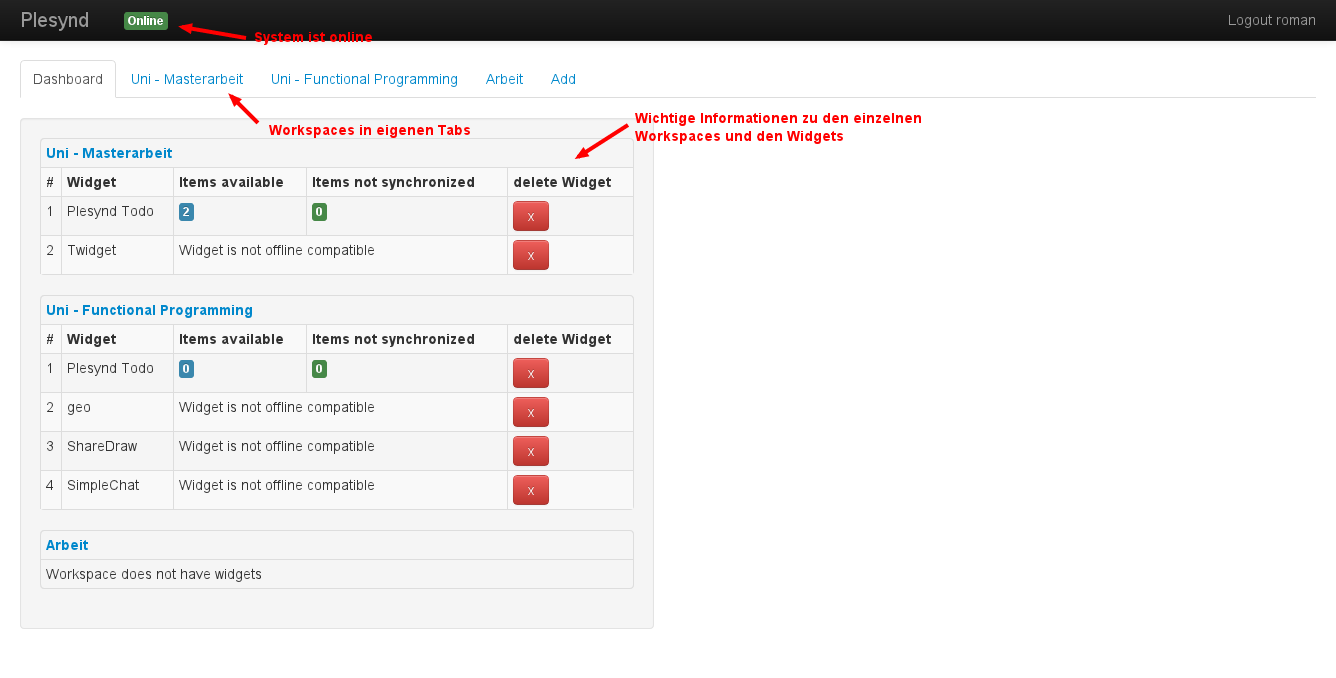
\includegraphics[]{./Figures/plesynd_dashboard.png}
    \rule{35em}{0.5pt}
  \caption[Plesynd User"=Interface: Dashboard]{Das Dashboard fasst die wichtigsten Informationen zusammen.}
  \label{fig:plesynd_dashboard}
\end{figure}

\begin{figure}
  \centering
  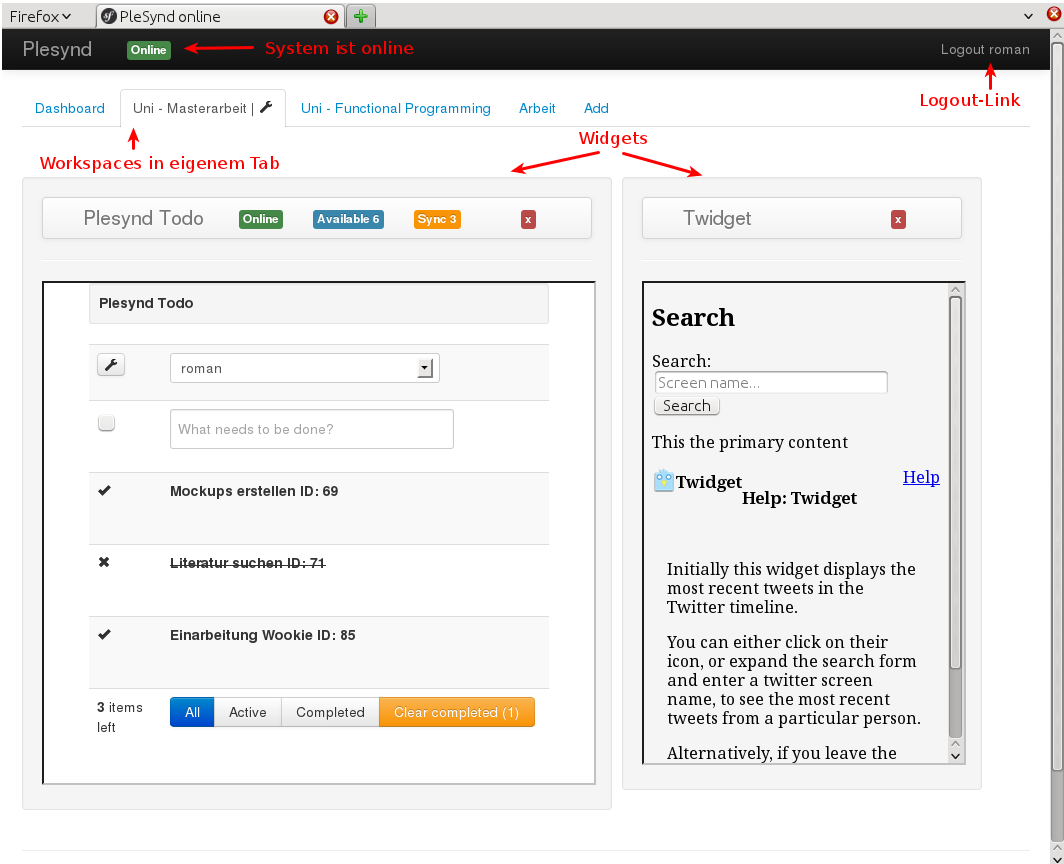
\includegraphics[]{./Figures/plesynd_workspace_online.png}
    \rule{35em}{0.5pt}
  \caption[Plesynd User"=Interface: Workspace Online]{Ein Workspace mit unterschiedlichen Widgets}
  \label{fig:plesynd_workspace_online}
\end{figure}

\begin{figure}
  \centering
  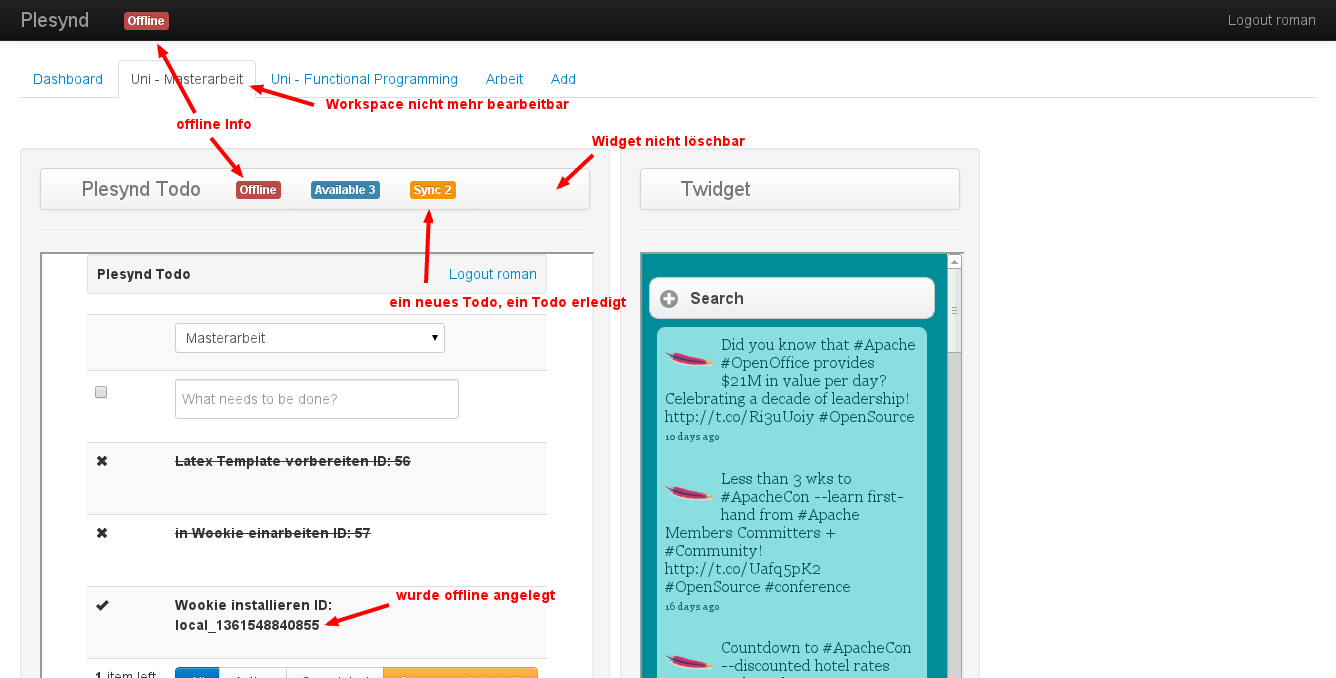
\includegraphics[]{./Figures/plesynd_workspace_offline.png}
    \rule{35em}{0.5pt}
  \caption[Plesynd User"=Interface: Workspace Offline]{Die wichtigsten Unterschiede im Offline"=Modus}
  \label{fig:plesynd_workspace_offline}
\end{figure}

\begin{figure}
  \centering
  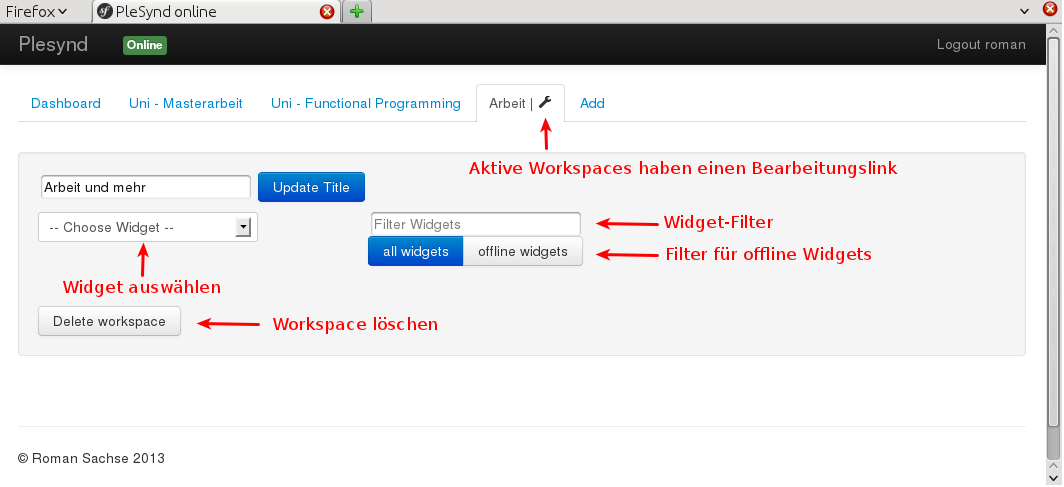
\includegraphics[]{./Figures/plesynd_workspace_edit.png}
    \rule{35em}{0.5pt}
  \caption[Plesynd User"=Interface: Bearbeiten von Workspaces]{Workspaces können direkt bearbeitet werden.}
  \label{fig:plesynd_workspace_edit}
\end{figure}

Zusammenfassend wurde für diese Arbeit mit Plesynd sowohl das Frontend als auch das Backend einer neuen Personal Learning Environment von Grund auf entworfen und auf Basis aktueller Webtechnologien implementiert.
 % Lösungsansatz

\chapter{Details zur Lösung / Validierung der Anforderungen}\label{chapter:Kapitel6}

\section{Entwicklungsumgebung und eingesetzte Werkzeuge}\label{section:entwicklungsumgebungen_tools}
Für die Entwicklung von Plesynd wurden unterschiedliche Tools und Frameworks genutzt. Entwickelt wurde das System auf Serverseite mit \acs{PHP} (\aclu{PHP}). Der clientseitige Code wurde mit Javascript implementiert. Die für die Entwicklung von Plesynd eingesetzten Frameworks werden im Folgenden kurz vorgestellt.

\subsection{AngularJS}\label{section:angularjs}
Plesynd ist eine größtenteils clientbasierte Applikation. Für die Implementierung des Systems fiel die Wahl auf das von Google entwickelte Javascript-Framework \href{http://angularjs.org/}{AngularJS}\footnote{weitere Informationen auf: \url{http://angularjs.org/}}. Im Gegensatz zu anderen Javascript-Frameworks verfolgt AngularJS für die Umsetzung des User Interfaces einen Ansatz, welcher am einfachsten als eine Erweiterung der Möglichkeiten von \ac{HTML} zu beschreiben ist. Hierfür bietet AngularJS sogenannte Direktiven. Diese erlauben die deklarative Angabe von Kontrollstrukturen wie Schleifen (inklusive Filtermechanismen) und konditionalen Anweisungen innerhalb des \ac{HTML}-Codes. AngularJS ist in der Lage dieses erweiterte \ac{HTML} zu parsen, auszuwerten und dem Anwender die Ergebnisse zu präsentieren. Der Entwickler kann auch eigene Direktiven für weitere \ac{DOM}-Manipulation entwickeln. Neben den Direktiven bietet AngularJS die Möglichkeit sogenannte Controller zu erstellen. In diesen Controllern wird die eigentliche Programmlogik ausgeführt. Ein Controller wird (ebenfalls über eine Direktive) einem beliebigen \ac{DOM}-Knoten zugewiesen. Auf die Variablen, die innerhalb des Controllers definiert wurden kann dann im Inhalt des \ac{DOM}-Elements zugegriffen werden. Durch die Funktionalität des sogenannten "`Two-Way-Data-Bindings"' sorgt AngularJS dafür, dass eine Änderung der Variable innerhalb des Controllers direkt im User Interface sichtbar wird. Ändert der Anwender auf der anderen Seite den Wert einer so gebundenen Variable (z.B. über ein Formularfeld), so spiegelt sich diese Änderung direkt im Wert der Variable im Controller wider. Somit erreicht Angular eine saubere Trennung zwischen der Business-Logik der Anwendung, dem User Interface und der manchmal recht komplexen Manipulation von \ac{DOM}-Elementen. Funktionalitäten, welche in mehreren Controllern oder auch in Direktiven benötigt werden, lassen sich in sogenannten Services implementieren. Mögliche Anwendungsfälle hierfür sind unter anderem das Kapseln von \ac{HTTP}-Requests oder die Arbeit mit einem Offline-Storage. Zusammenfassend bietet AngularJS:
\begin{itemize}
 \item \emph{Direktiven} zur Manipulation des \ac{DOM}
 \item \emph{Controller} zur Ausführung der Programmlogik und Reaktion auf Nutzereingaben
 \item \emph{Services} zur Kapselung von Funktionalitäten, die an multiplen Stellen benötigt werden
\end{itemize}
Es ist möglich, dass Abhängigkeiten zwischen den einzelnen Bestandteilen existieren. Ein Controller benötigt z.B. zumeist unterschiedliche Services für den korrekten Ablauf der Programmlogik. Diese Abhängigkeiten werden deklarativ angegeben. AngularJS sorgt dann per Dependency-Injection-Mechanismus dafür, dass die Objekte ihre Abhängigkeiten erhalten. AngularJS bietet noch einige andere Funktionalitäten, wie z.B. ein Event-System und das Beobachten beliebiger Objekt-Eigenschaften, welche jedoch aus Gründen des Umfangs hier nicht weiter vorgestellt werden.

Im Folgenden verdeutlicht ein kurzes Beispiel die Arbeit mit AngularJS. Das Beispiel ist an dem für die Arbeit entwickelten Todo-Widget angelehnt. Es zeigt einen Controller und einen Ausschnitt \ac{HTML}-Quellcode.

\begin{lstlisting}
Application.Controllers.controller('TodoCtrl', ['$scope', 'todoService', function ($scope, todoService) {
  $scope.todos = [
    {id: 1, content: 'Todo 1', completed : false},
    {id: 2, content: 'Todo 2', completed : false},
    {id: 3, content: 'Todo 3', completed : true},
  ];
  
  $scope.newTodo = '';
  $scope.addTodo = function () {
    if ($scope.newTodo.length === 0) { return; }

    var todo = {title : $scope.newTodo, completed : false,};
    todoService.post(todo, function () {
      $scope.todos.push(todo);
      $scope.newTodo = '';
    });
  };
  $scope.todoCompleted = function (todo) {
    todo.completed = !todo.completed
    todoService.put(todo);
  };
});
\end{lstlisting}
Der Controller hat den Namen \texttt{TodoCtrl}. Seine Definition verlangt die Injektion zweier Services. Zum einen des AngularJS internen \texttt{\$scope} Service, zum anderen des eigenen \texttt{todoService}. Alle Variablen, die im Controller definiert werden und im \ac{HTML} zur Verfügung stehen sollen, werden dem \texttt{\$scope} Objekt als Eigenschaften zugewiesen. Hierzu gehören einige Todo-Objekte (welche auch vom Server geholt werden könnten), ein String für ein neues Todo und zwei Funktionen zum Hinzufügen und Bearbeiten von Todos. Das folgende \ac{HTML} wird über die Direktive \texttt{ng-controller} mit dem Controller verknüpft.

\begin{lstlisting}
<div ng-controller="TodoCtrl">
 <table>
  <tr>
   <td colspan="2">
    <form ng-submit="addTodo()">
     <input type="text" placeholder="What needs to be done?" ng-model="newTodo" autofocus>
    </form>
   </td>
  </tr>
  <tr ng-repeat="todo in todos>
   <td>
    <i ng-hide="todo.completed" class="icon-ok" ng-click="todoCompleted(todo)"></i>
    <i ng-show="todo.completed" class="icon-remove" ng-click="todoCompleted(todo)"></i>
   </td>
   <td>
    <strong>Title: {{todo.title}} (Id: {{todo.id}})</strong>
   </td>
  </tr>
 </table>
</div>
\end{lstlisting}
Im \ac{HTML} wird die Direktive \texttt{ng-repeat} dazu genutzt, die im Controller hinterlegten Todo Objekte zu durchlaufen. Mit der Klammersyntax (z.B. \{\{todo.title\}\}) wird der Wert einer Variable oder einer Objekteigenschaft ausgegeben. Die Direktiven \texttt{ng-show} und \texttt{ng-hide} blenden ein \ac{DOM}-Element ein oder aus, wenn angegebene Bedingung zu \texttt{true} auswertet. Mit einem Klick auf ein Icon, welches mit der \texttt{ng-click} Direktive ausgezeichnet wurde, wird die \texttt{todoCompleted} Methode im Controller aufgerufen, welches das aktuelle Todo-Objekt aktualisiert. Das im oberen Teil des Quellcodes abgebildete Formular dient zum Hinzufügen eines neuen Todo-Objektes. Das Input-Feld wird mit der \texttt{ng-model} Direktive mit der Variable \texttt{\$scope.newTodo} verknüpft. Trägt der Anwender etwas in das Formularfeld ein, ändert sich diese Variable automatisch im Controller. Der Controller initialisiert sie mit einem leeren String, so dass im Formularfeld kein vorausgefüllter Wert steht. Beim Abschicken des Formulars wird die in der \texttt{ng-submit} Direktive angegebene Methode \texttt{\$scope.addTodo} aufgerufen, welche auf Basis des eingegebenen Wertes für \texttt{\$scope.newTodo} und mit Hilfe des \texttt{todoService} ein neues Todo-Objekt erstellt und zur Kollektion hinzufügt. Auf Grund des oben erwähnten "`Two-Way-Data-Bindings"' wird das neue Todo automatisch in die über \texttt{ng-repeat} erstellte Liste der Todos aufgenommen. Der Entwickler muss sich nicht um etwaige \ac{DOM}-Manipulationen kümmern, so dass die Anwendungslogik hiervon völlig unberührt bleibt.

\subsection{Symfony2}\label{section:symfony2}
\href{http://symfony.com}{Symfony2}\footnote{weitere Informationen auf: \url{http://symfony.com}} ist ein in \ac{PHP} implementiertes komponenten\allowbreak basiertes Framework zur Entwicklung von \ac{MVC} Anwendungen. Zu den bereitgestellten Komponenten gehört beispielsweise ein Service Container. Dieser erlaubt es die von den genutzten Klassen benötigten Abhängigkeiten zu definieren. Der Container sorgt dann für eine Instantiierung der Abhängigkeiten und ein Injizieren\footnote{Dies ist eine Art der Umsetzung des Dependency Injection Design-Patterns. Dieses Muster wird dazu verwendet, um eine stärkere Entkopplung zwischen einzelnen Objekte in der objektorientierten Programmierung zu erreichen. Anstatt die Abhängigkeiten fest in einer Klasse zu verankern (in dem das benötigte Objekt in der Klasse instantiiert wird), gibt die Klasse entweder im Konstruktor oder in Setter-Methoden nur das Interface des benötigten Objektes an. Dies ermöglicht ein einfacheres Austauschen der eigentlichen Implementierung und kann insbesondere die Arbeit mit Unit Tests erleichtern (vgl. \cite{Fowler2004})} dieser zur Laufzeit. Des Weiteren bietet Symfony2 unter anderem die eigene Template-Engine \href{http://twig.sensiolabs.org/}{Twig}\footnote{weitere Informationen auf: \url{http://twig.sensiolabs.org/}}, sowie ein Event"=Listener System, welches ermöglicht auf bestimmte Events zu reagieren. Ein Beispiel hierfür wäre das \texttt{onKernelResponse} Event, welches in der Lage ist die Antwort, die das System an den Client schickt, zu verändern, um beispielsweise zusätzliche Header zu setzen. Das Model wird in Symfony2 standardmäßig über Doctrine2 (siehe Abschnitt \ref{section:doctrine2}) abgebildet.
Die Komponenten werden in Symfony2 über sogenannte Bundles implementiert. Bundles sind von dem System unabhängige Plugins, mit einer festen Verzeichnisstruktur, welche einfach in eine Applikation eingebunden werden können. Das besondere an Symfony2 ist, dass das gesamte System aus Bundles aufgebaut ist. Hierzu gehören also auch das Kern-Framework, alle Komponenten, zusätzlicher Third-Party-Code sowie die eigene Applikation selbst (vgl. \cite{Symfony2Bundles}).

\subsection{Doctrine2}\label{section:doctrine2}
Für die serverseitige Speicherung der unterschiedlichen Daten (Workspace, Widgets, Todos etc.) wird Doctrine2 genutzt. Doctrine2 ist ein Werkzeug zur objektrelationalen Abbildung von einfachen Objekten in relationale Datenbanken (\ac{ORM}). Doctrine2 nutzt im Gegensatz zu vielen anderen \ac{ORM}"=Systemen, nicht das Active"=Record"=Pattern, sondern das Data-Mapper-Pattern. Der entscheidende Unterschied hierbei ist der, das die Objekte selber keine Methoden besitzen, mit denen sie in der Datenbank hinterlegt oder gefunden werden können, sie können als einfach Objekte ohne besondere Fähigkeiten implementiert werden (vgl. \cite{Fowler2002}). Diese Arbeit übernimmt eine Abstraktionsebene zwischen den Objekten und der Datenbank, bei Doctrine2 ein sogenannter Entity"=Manager. Dieser ist in der Lage zu erkennen, ob bestimmte Objekte schon in den Speicher geladen wurden. Ist dies nicht der Fall kann er sie mitsamt eventueller Verknüpfungen aus der Datenbank in den Speicher laden und dem System zur Verfügung stellen. Somit können sich die Objekte allein mit der Geschäftslogik des Systems beschäftigen, wodurch eine bessere Entkopplung der Zuständigkeiten (Geschäftslogik und Speichern in einer relationalen Datenbank) der einzelnen Teile des Systems erreicht wird.

\subsection{jQuery}
\href{http://jquery.com/}{jQuery}\footnote{weitere Informationen auf: \url{http://jquery.com/}} ist eine Javascript-Bibliothek zur einfachen Manipulation des \ac{DOM}. Des Weiteren stellt sie erweiterte Javascript-Funktionalitäten zur Verfügung und vereinfacht die Arbeit mit dem browserbasierten Event-System. In Plesynd basiert unter anderem das Postmessage-Plugin (siehe Abschnitt \ref{section:kommunikation_zwischen_iframes_implementierung}) auf jQuery. AngularJS nutzt jQuery, wenn es vorhanden ist zur \ac{DOM}-Manipulation. Ist jQuery nicht geladen benutzt es hierfür ein eigenes rudimentäres Plugin.

\subsection{Twitter Bootstrap}
\href{http://twitter.github.com/bootstrap/}{Twitter Bootstrap}\footnote{weitere Informationen auf: \url{http://twitter.github.com/bootstrap/}} ist ein von Twitter entwickeltes Framework zur schnellen und einfachen Entwicklung von Frontends. Es stellt \ac{CSS}-Vorlagen und Javascript-Komponenten zur Verfügung, welche es dem Entwickler ermöglichen sollen, in kurzer Zeit ein User"=Interface zu entwerfen und umzusetzen. Bootstrap beinhaltet \ac{CSS}-Vorlagen für Grids, Tabellen, Buttons etc. In Plesynd wird von den von Bootstrap zur Verfügung gestellten Javascript-Komponenten momentan nur die \href{http://twitter.github.com/bootstrap/javascript.htmlmodals}{Modal-Komponente}\footnote{weitere Informationen auf: \url{http://twitter.github.com/bootstrap/javascript.htmlmodals}} verwendet. 

\section{Implementierungsdetails}\label{section:implementierungsdetails}

\subsection{eigene Symfony2 Bundles}\label{section:backend}
Für die Umsetzung von Plesynd wurden auf der Serverseite fünf Symfony2-Bundles implementiert. Diese werden im Folgenden kurz vorgestellt:

\begin{itemize}
\item Das \texttt{CorujaPlesyndBundle} bildet das Herzstück des Plesynd-System. Es enthält die zentralen \texttt{Workspace}- und \texttt{Widget}-Entitäten, in denen der größte Teil der Geschäftslogik für die Arbeit mit Plesynd abgebildet wird. Zusätzlich gibt es noch Controller, die für die \texttt{Workspace}- und \texttt{Widget}-Controller, welche die REST-Anfragen des Clients entgegen nehmen und abarbeiten, und den \texttt{Plesynd}-Controller, welcher für das initiale Bereitstellen der benötigten Daten zuständig ist. Hier findet man auch die Javascript-Dateien, welche für die Arbeit mit den Widgets, den Workspaces und dem Dashboard notwendig sind.
\item Zur Kommunikation mit Wookie (siehe Abschnitt \ref{section:w3c_widgets}) wurde das \texttt{Coruja\allowbreak Wookie\allowbreak Connector\allowbreak Bundle} entwickelt. Dieses integriert das \href{http://wookie.apache.org/docs/embedding.html}{Wookie Connector Framework}\footnote{weitere Informationen auf: \url{http://wookie.apache.org/docs/embedding.html}} und versetzt das \texttt{CorujaPlesyndBundle} in die Lage, direkt Anfragen an Wookie zu versenden. Das Bundle ist über die normale Symfony2 Konfiguration konfigurierbar, so dass es mit unterschiedlichen Wookie-Instanzen kommunizieren kann.
\item Das \texttt{CorujaUserBundle} basiert auf dem \href{https://github.com/FriendsOfSymfony/FOSUserBundle}{FOSUserbundle}\footnote{weitere Informationen auf: \url{https://github.com/FriendsOfSymfony/FOSUserBundle}} und ist für das User"=Management in Plesynd zuständig.
\item Im \texttt{Coruja\allowbreak Angular\allowbreak Module\allowbreak Bundle} werden die AngularJS"=Implementierungen hinterlegt, welche sowohl für das Plesynd-System als auch für zusätzliche Widgets verwendet werden können. Hierzu gehören insbesondere das System, welches für die Offline-Fähigkeiten zuständig ist, aber auch Services für die Inter"=Frame"=Kommunikation oder die Verwendung von Http\allowbreak Xml\allowbreak Requests in Formularen.  
\item Für eine prototypische Implementierung eines offline fähigen Widgets wurde das \texttt{CorujaTodoBundle} entwickelt. Dieses arbeitet mit dem Todo-Widget zusammen, nimmt dessen REST-Anfragen entgegen und bearbeitet diese. Für das User"=Management nutzt es ebenfalls das CorujaUserBundle.
\end{itemize}

\subsection{Umsetzung der Offline-Fähigkeiten}\label{section:offline_faehigkeiten}

\subsubsection*{Information über Änderung des Online-Status}
Die Applikation wird über ein globales Event an zentraler Stelle darüber informiert, wenn sich der Online-Status des Browser ändert:
\begin{lstlisting}
// bei Erstaufruf der Applikation
.run(['$rootScope', '$window', function ($rootScope, $window) {
    // Status wird auf online geändert, offline funktioniert analog
    $window.addEventListener("online", function () {
        $rootScope.$apply(function () {
            // sende internes Event an alle Listener
            $rootScope.$broadcast('onlineChanged', true);
        });
    }, true);
\end{lstlisting}

Als Reaktion darauf wird ein internes Event ausgelöst, welches von den jeweiligen Listenern verarbeitet werden kann. Beispielsweise können die Controller mit der Änderung einer Variable reagieren, welche dann für das Ausblenden von \ac{DOM}-Elementen im Offline-Modus genutzt werden können:
\begin{lstlisting}
// im Plesynd Controller
$rootScope.$on('onlineChanged', function (evt, isOnline) {
  [...]
  $scope.isOnline = isOnline;
  [...]
});
\end{lstlisting}

\subsubsection*{Local Storage \ac{API}}
Wie oben beschrieben ist Plesynd in der Lage zu erkennen, wenn das System offline genutzt wird. Ist dies der Fall werden keine Requests mehr an den Server gesendet, sondern die Daten werden im Local-Storage (siehe Abschnitt \ref{section:offline_storage}) gespeichert. Für diese Funktionalität sind hauptsächlich zwei entwickelte AngularJS-Services zuständig: \texttt{Coruja\allowbreak Resource\allowbreak Service} und \texttt{Coruja\allowbreak Local\allowbreak Storage\allowbreak Service}. Da diese Services global genutzt und von allen Widgets und Applikationen eingebunden werden müssen, die die Offline-Fähigkeiten von Plesynd nutzen wollen, sind diese im CorujaAngularModuleBundle hinterlegt. Der \texttt{Coruja\allowbreak Local\allowbreak Storage\allowbreak Service} ist für das Speichern der Daten im Local-Storage zuständig. Der \texttt{Coruja\allowbreak Resource\allowbreak Service} kapselt den \texttt{Coruja\allowbreak Local\allowbreak Storage\allowbreak Service} und ein AngularJS \texttt{\$ressource}-Service-Objekt, welches eine Abstraktionsebene für REST-Anfragen an einen Server darstellt. Der \texttt{Coruja\allowbreak Resource\allowbreak Service} erkennt mit Hilfe des \texttt{Coruja\allowbreak Online\allowbreak Status\allowbreak Service}, ob das System zum Zeitpunkt einer Anfrage online oder offline ist und benutzt dann, je nach Situation, einen oder beide gekapselten Services zum Ausführen der Anfrage. Ist das System offline, wird nur der \texttt{Coruja\allowbreak Local\allowbreak Storage\allowbreak Service} verwendet. Ist das System online, wird ein Request an den Server gesendet. Damit das System bei einem Ausfall der Internetverbindung weiter arbeiten kann, wird ebenfalls der Local-Storage aktualisiert. Tritt aus irgend einem Grund ein Fehler bei der Kommunikation mit dem Server auf wird die Anfrage trotzdem im Local-Storage hinterlegt. Der \texttt{Coruja\allowbreak Resource\allowbreak Service} wird ebenfalls verwendet, um die Synchronisation zwischen dem Local-Storage und dem Server vorzunehmen, sobald das System wieder online ist. 

Im folgenden Beispiel sieht man einen Ausschnitt der Bearbeitung einer PUT Anfrage, also dem Update einer Ressource, bei dem das eben beschriebene Prinzip zum Einsatz kommt:
\begin{lstlisting}
resource.put = function (item, success, error) {
    resourceDeferred = $q.defer();
    var promise = resourceDeferred.promise;

    // wenn nicht online, schreibe in Local-Storage
    if (!onlineStatus.isOnline()) {
        resource.localFallback(item, 'put', success, error);
        return promise;
    }
    // sende Anfrage an Server
    remoteResource.put(item,
        function (data, header) {
	    // update Local-Storage im Erfolgsfall
            resource.updateLocalStorage(item, 'put');
            resourceDeferred.resolve();
            (success || noop)(item, header);
        }, function (response) {
	    // speichere auch im Local-Storage bei Fehler
            resource.localFallback(item, 'put', success, error, response);
        });
    return promise;
}; 
\end{lstlisting}
\texttt{CorujaLocalStorageService} stellt für die Arbeit mit Ressourcen ein Interface bereit, welches an die in Abschnitt (\ref{section:rest}) beschriebenen \ac{HTTP}-Methoden angelehnt ist:
\begin{lstlisting}           
interface ResourceStorage {
  // holt alle Ressourcen anhand der Parameter
  array query(array params, callback success, callback error)
  // holt eine Ressource anhand der Parameter
  object get(array params, callback success, callback error)  
  // erstellt eine neue Ressource
  promise post(object item, callback success, callback error)
  // updated eine Ressource
  promise put(object item, callback success, callback error) 
  // entfernt eine Ressource
  promise delete(object item, callback success, callback error) 
  // Synchronisiert den Local-Storage mit dem Server
  void synchronize(callback success, callback error)
};             
\end{lstlisting}

Damit die Offline-Funktionalität für einen vom Server zur Verfügung gestellten Ressourcentyp (z.B. Todo, Todo-Liste, Widget, Workspace) genutzt werden kann, muss für jeden Typ ein eigener Service auf Basis des beschriebenen Interfaces implementiert werden. Dieser Service kapselt den oben beschriebenen \texttt{CorujaResourceService} und stellt eine \ac{API} für die Arbeit mit diesen Ressourcen in den Controllern, Services und Direktiven bereit. Die Services für die einzelnen Ressourcentypen können diese Methoden zur Nutzung in einem Controller freigeben, müssen dies aber nicht zwingend. Sie können diese auch umbenennen oder eigene Methoden hinzufügen, müssen diese dann jedoch intern auf Basis des \texttt{ResourceStorage} Interfaces implementieren. Innerhalb der Controller wird nur mit diesem Service gearbeitet, für den Entwickler ist die Unterscheidung zwischen Onlinestatus und Offline-Status in dieser Hinsicht also vollkommen transparent. Im Folgenden werden Auszüge aus dem \texttt{TodoService} gezeigt, welcher den \texttt{CorujaResourceService} wie beschrieben nutzt. Zuerst wird der Local-Storage und der Service für die REST-Anfragen konfiguriert und auf Basis dieser Konfiguration eine Instanz der \texttt{CorujaResourceService} erstellt. Dieser wird dann in den Methoden query, put, synchronize etc. verwendet. Die hier definierten Methoden stehen dann in einem Controller zur Verfügung, wenn dieser den \texttt{TodoService} als Abhängigkeit angibt (siehe Listing in Kapitel \ref{section:angularjs}).
\begin{lstlisting}
Application.Services.factory('todoService', function ($resource, [...], localStorage, resourceService,  configuration) {
  [...]
  // Konfigurere den Local Storage und den $resource Service
  config = {
    remoteResource : $resource(configuration.TODO_RESOURCE_URI, {todoId:'@id'}, {
      put:{method:'PUT' },
      post:{method:'POST' }
    }),
    localResource : localStorage(local_storage_prefix),
    // dieser Service benutzt Synchronisation
    use_synchronization : true
  };   
  // erstelle auf Basis der Konfiguration eine Instanz des resourceService
  resource = resourceService(config);
    
  service.query = function (success, error) {
    return resource.query({}, success, error);
  }; 
  [...]
  service.put = function (item, success, error) {
      resource.put(item, success, error).then(resolver, resolver);
  };  
  service.synchronize = function (success, error) {
      resource.synchronize(success, error);
  };
  return service;
}]);
\end{lstlisting}

\subsubsection*{Einschränkungen im Offline-Betrieb}
Trotz der Offline-Fähigkeiten des System stehen im Offline-Betrieb nicht alle Funktionalitäten zur Verfügung. Hauptaugenmerk wurde auf die Weiterbenutzbarkeit der Widgets im Offline-Modus gelegt. Im Folgenden sind einige Funktionen aufgelistet, welche während des Offline-Betriebes deaktiviert werden.
\begin{itemize}
 \item Hinzufügen, Bearbeiten und Löschen von Widgets
 \item Hinzufügen, Bearbeiten und Löschen von Workspaces
 \item Drag and Drop von Widgets
 \item Anlegen und Bearbeiten von Todo-Listen im Todo-Widget
\end{itemize}
 Die Funktionalitäten werden meist einfach über eine \texttt{ng-show} Direktive ausgeblendet, sobald das System feststellt, dass es sich im Offline-Modus befindet. Im folgenden Listing wird beispielsweise die Funktionalität zum Löschen von Widgets aus Workspaces aus dem User Interface entfernt:
\begin{lstlisting}
<ul class="nav pull-right">
 <li>
  <a ng-show="isOnline" ng-click="deleteWidget(widget)">
   <span class="label label-important">x</span>
  </a>
 </li>
</ul>
\end{lstlisting}

\subsubsection*{Preloads der Widgets}
Plesynd muss den User in die Lage versetzen nach einmaligem Laden des Systems offline weiterzuarbeiten. Dies ist nur möglich, wenn alle Daten beim erstmaligen Aufruf geladen werden. Insbesondere gilt dies für die iframes der Widgets. Es müssen die Appcache-Dateien der einzelnen Widgets geladen werden und das Dashboard benötigt die Informationen der Widgets zur Ausgabe der zusammenfassenden Informationen direkt bei Systemstart. Der Nutzer soll sich nicht erst durch alle vorhandenen Workspaces bewegen müssen, um die Daten aller Widgets zu laden. Aus diesem Grund müssen die iframes aller Widgets der Workspaces bei dem ersten Aufruf im \ac{DOM} vorhanden sein. Des Weiteren dürfen die iframes bei Wechsel zwischen den Workspaces nicht wieder aus dem \ac{DOM} entfernt werden. Der Grund hierfür ist, dass bei Wechsel des Online-Status alle iframes aktualisiert werden müssen und nicht nur diejenigen des aktuellen Workspaces.

Aus diesen Gründen wurde entschieden alle iframes bei Systemstart direkt zu laden und im \ac{DOM} vorzuhalten. Es findet lediglich eine Filterung auf Basis des anzuzeigenden Workspace statt, welche der iframes ausgegeben werden und welche ausgeblendet werden.
\begin{lstlisting}
// im Controller
$scope.isWidgetVisible = function (widget) {
  return widget.workspace.id === $scope.activeWorkspace.id;
};
// im HTML
<div ng-repeat="widget in widgets" ng-show="isWidgetVisible(widget)" ...>
\end{lstlisting}

\subsection{Widgets auf der Hauptebene}
Die ursprüngliche Architektur von Plesynd sah vor, dass der Local-Storage nur direkten Zugriff auf die Hauptdatensätze liefert. Dies hätte zur Folge, dass nur Workspaces direkt referenziert werden können. Der Zugriff auf die Widgets würde dann über ihre Workspaces erfolgen. Das entwickelte Storage/Resource System kann auf Grund der Einfachheit des Local-Storage jedoch nur mit Hauptdatensätzen arbeiten. Dieses Vorgehen hat jedoch einige Probleme und Fragen nach sich gezogen: 
\begin{itemize}
 \item Wie kann man lokal mit Subdatensätzen arbeiten, wenn man keinen direkten Zugriff auf sie hat? Es ist nicht ohne weiteres möglich aus dem Local-Storage eines Workspaces ein Widget zu löschen oder zu bearbeiten. Der Workspace müsste geholt, das Widget in dem Workspace gelöscht/bearbeitet und der Workspace wieder geschrieben werden. 
 \item Als REST-Service wäre es kein Problem direkt Widgets zu löschen oder zu bearbeiten, aber dies geht nicht ohne weiteres im Local-Storage. Der Local-Storage muss aber aktualisiert werden, damit das System auch offline mit den korrekten Daten arbeitet.
\end{itemize} 

Es gibt mehrere Möglichkeiten dieses Problem zu lösen:
\begin{enumerate}
 \item\label{enumerate:widgets_hauptebene_indexed_db} Umstellung auf eine andere Lösung zur lokalen Speicherung der Daten (z.B. IndexedDb).
 \item\label{enumerate:widgets_hauptebene_erweiterung_local_storage} Erweiterung der Implementierung zur Speicherung der Daten im Local-Storage, so dass auch Subeinträge gefunden und bearbeitet werden können.
 \item\label{enumerate:widgets_auf_hauptebene} Speicherung der Subdatensätze auf der Hauptebene. Alle direkt über die REST-Schnittstelle ansprechbaren Ressourcen werden auf der Hauptebene im Local-Storage hinterlegt, Widgets werden also auch auf der Hauptebene im Local-Storage gespeichert.
\end{enumerate}
Punkt \ref{enumerate:widgets_hauptebene_indexed_db} sollte auf Grund der höheren Komplexität vermieden werden. Punkt \ref{enumerate:widgets_hauptebene_erweiterung_local_storage} kam in die engere Betrachtung wurde jedoch verworfen, da er die Komplexität der Speicherung in den Local-Storage beträchtlich erhöht hätte. Wie in Abschnitt \ref{section:plesynd_architektur} beschrieben, sollte es für die Implementierung der Logik unerheblich sein, ob das System zum Zeitpunkt einer Nutzeraktion online oder offline ist. Um dies mit Punkt \ref{enumerate:widgets_hauptebene_erweiterung_local_storage} zu erreichen, hätte die in \ref{section:offline_faehigkeiten} vorgestellte Vorgehensweise grundlegend geändert werden müssen. Aus diesen Gründen wurde Punkt \ref{enumerate:widgets_auf_hauptebene} umgesetzt. Jede REST-Ressource wird direkt auf der Hauptebene abgelegt. Somit ergibt sich eine einfache 1:1 Abbildung der Ressourcen auf den Local-Storage. 

\subsection{Probleme bei multiplen Instanzen des selben Widgets}
Es ist möglich, dass das selbe Widget mehrfach in einer Plesynd-Instanz verwendet wird. Beispielsweise könnte das Todo-List-Widget auf mehreren Workspaces verwendet werden, um je nach Kontext unterschiedliche Todo-Listen zu verwalten. Es können hierbei jedoch Synchronisationsprobleme auftreten, wenn beide Widget-Instanzen offline auf der selben Datenbasis operieren. Der Grund dafür liegt darin, dass die POST-Methode nicht idempotent ist (siehe Abschnitt \ref{section:rest}). Da die unterschiedlichen Widget-Instanzen nicht in Kommunikation miteinander stehen, bedeutet dies im Falle einer Synchronisierung, dass beide Instanzen lokal hinzugefügte Datensätze per POST an den Server schicken. Somit entstehen nicht gewollte Dopplungen der Datensätze. DELETE und PUT Aufrufe stellen für diesem Fall keine Probleme dar, da diese Methoden idempotent sind und ein doppelter DELETE Request an eine Ressource keine negativen Auswirken hat. Dieses Problem wurde gelöst, in dem jede Widget-Instanz seinen eigenen Local-Storage zur Speicherung seiner Daten erhält. Der Name des Local-Storage ergibt sich aus dem internen Namen des Widgets (beispielsweise todo) konkateniert mit dem Namen des iframes in dem das Widget aufgerufen wird. Der Name des iframes ergibt sich aus der ID, welche Wookie für jedes Widgets erstellt. Diese ID ist einzigartig und verändert sich auch bei wiederholtem Aufrufen nicht. Somit ist sichergestellt, dass jedes Widget einen festen Local-Storage erhält.

Es ist natürlich möglich, dass unterschiedliche Widget-Instanzen zwar unterschiedlichen Local-Storage benutzen, jedoch auf der selben Datenbasis arbeiten (beispielsweise die selben Todo-Listen verwenden). Da momentan noch keine Inter-Widget Kommunikation stattfindet, kann es hierbei zu Problemen kommen, wenn im Offline Betrieb beispielsweise ein Datensatz in einer Instanz gelöscht wird, während er in einer anderen bearbeitet wurde. Dieses Problem wurde im Rahmen dieser Arbeit nicht weiter betrachtet und sollte eventuell in Folgearbeiten bearbeitet werden.

\subsection{Drag and Drop}
Zur Umsetzung der Drag and Drop Funktionalität zum Sortieren der Widgets auf einem Workspace wurde das \href{http://jqueryui.com/sortable/}{Sortable Widget}\footnote{weitere Informationen auf: \url{http://jqueryui.com/sortable/}} der \href{http://jqueryui.com}{jQueryUi-Bibliothek}\footnote{weitere Informationen auf: \url{http://jqueryui.com}} verwendet. Diese wurde in einer eigenen AngularJS-Direktive gekapselt, so dass das jQueryUi-Widget in der bestehenden Architektur verwendet werden konnte. Die Direktive verwendet den \texttt{WidgetService}, um die neue Position der Widgets dem Server mitzuteilen und den \texttt{Online\allowbreak Status\allowbreak Service}, um die Drag and Drop Funktionalität im Offline-Modus zu deaktivieren.

\subsection{\ac{CORS}}\label{section:cors_implementierung}
In einer Mashup-Anwendungen wie Plesynd ist es unumgänglich, dass XMLHttp Requests versendet werden. Insbesondere die Wookie-Instanz und dadurch die Origin aller Widgets unterscheidet sich von der Origin des eigentlichen Plesynd-Systems. Aus diesem Grund benötigt Plesynd eine \ac{CORS} (siehe Abschnitt \ref{section:same_origin_policy}) Implementierung. Zur Vereinfachung der Umsetzung wird das \href{https://github.com/nelmio/NelmioCorsBundle}{NelmioCorsBundle}\footnote{weitere Informationen auf: \url{https://github.com/nelmio/NelmioCorsBundle}} verwendet. Dieses erlaubt in der Systemkonfiguration die gewünschten Einstellungen vorzunehmen. Im Folgenden wird beispielhaft die Konfiguration für das Todo-Widget gezeigt: 
\begin{lstlisting}
nelmio_cors:
  paths:
    '^/(todo/api|login|logout)':
      allow_origin: ['*']
      allow_headers: ['X-REQUESTED-WITH', 'Content-Type', 'Authorization']
      allow_methods: ['POST', 'PUT', 'GET', 'DELETE', 'OPTIONS'],
      expose_headers: ['Location']
\end{lstlisting}
Allen Requests, die an eine \ac{URI} gehen, welche mit /todo/api oder /login oder /logout beginnen, wird hierbei erlaubt von einer anderen Quelle zu kommen. Es werden die Header und Methoden definiert, welche in einem solchen Request erlaubt sind. Der Location Header wird bei Antwort dem Client wieder zur Verfügung gestellt. Dieser wird benutzt, um nach dem Erstellen einer neuen Ressource per POST die \ac{URI} der Ressource an den Client zu übermitteln. 

\subsection{Kommunikation zwischen den iframes}\label{section:kommunikation_zwischen_iframes_implementierung}
Sobald ein neues offline fähiges Widget einem Workspace hinzugefügt wird, meldet sich dieses bei Plesynd an. Nun ist es möglich, dass es Plesynd über die in dem Widget verwalteten Datensätze informiert. Da die Widgets als iframes realisiert wurden, welche eine andere Origin als Plesynd benutzen, muss das Postmessage System (siehe Kapitel \ref{section:same_origin_policy}) zur Interframe-Kommunikation implementiert werden. In Plesynd wird hierbei das \href{https://github.com/daepark/postmessage}{postmessage}\footnote{weitere Informationen auf: \url{https://github.com/daepark/postmessage}} jQuery-Plugin genutzt. Dieses stellt Methoden bereit, welche das Binden an Nachrichten-Events und das Versenden von Nachrichten erlauben. Die Widgets-Seite registriert sich bei Erstaufruf mit Plesynd und kann später die Nachrichtenfunktion des \texttt{childFrameMessenger}-Services benutzen:
\begin{lstlisting}
// bei Erstaufruf
.run([..., 'childFrameMessenger', function (..., childFrameMessenger) {
    childFrameMessenger.registerWithParent();
// im TodoService, nach Hinzufuegen eines TodoService
service.post = function (item, success, error) {
  resource.post(item, success, error);
  service.notifyParentAboutItems();
};
// Definition im childFrameMessenger Service //
// registriere bei Plesynd
ChildFrameMessenger.prototype.registerWithParent = function () {
    pm({
        target : $window.parent,
        type   : "register_child_frame",
        data   : {id : this.name}
    });
};
// sende Infos an Plesynd
ChildFrameMessenger.prototype.notifyParentAboutItems = function (data) {
    data.id = this.name;
    pm({
        target : $window.parent,
        type   : "notify_about_items",
        data   : data
    });
};
\end{lstlisting}

Plesynd ist in der Lage auf die versendeten Nachrichten zu hören und dann die Informationen im Dashboard und in der Kopfzeile der einzelnen Widgets darzustellen:
\begin{lstlisting}
// Definition im ParentFrameMessenger Service
ParentFrameMessenger.prototype.initialize = function () {
    // Listener: Registrieren von Widgets
    pm.bind("register_child_frame", function (child) {
        if (child['id'] != undefined) {
            $rootScope.$broadcast("childFrameRegistered", child);
        }
    });
    // Listener: eingehende Daten
    pm.bind("notify_about_items", function (data) {
        if (data['id'] != undefined) {
            $rootScope.$broadcast("incomingFrameData", data);
        }
    });
};
\end{lstlisting}

\section{Validierung der Anforderungen}\label{section:validierung_der_anforderungen}
In diesem Abschnitt wird die in Kapitel \ref{chapter:Kapitel5} vorgestellte Lösung analysiert und auf die Erfüllung der in Kapitel \ref{chapter:Kapitel3} aufgestellten Anforderungen hin untersucht. Die nichtfunktionalen Anforderungen werden argumentativ auf Basis des umgesetzten Systems validiert. In Abschnitt \ref{section:umsetzung} wurde die Umsetzung der funktionalen Anforderungen mit Hilfe von Mockups beschrieben. Diese Mockups wurden, wie dargestellt, im implementierten System umgesetzt, so dass die erwähnten funktionalen Anforderungen als validiert betrachtet werden. Im Folgenden wird deshalb nur noch auf Anforderungen eingegangen, die nicht komplett erfüllt wurden, oder deren Umsetzung noch in zukünftigen Arbeiten erweitert werden könnte.

\subsection{Validierung der funktionalen Anforderungen}\label{section:funktionale_anforderungen_validierung}
\textbullet{} \reqref{requirementKeinZugriffNachLogout} (\emph{\requirementKeinZugriffNachLogout})\\
Wie in Abschnitt \ref{section:umsetzung} beschrieben, wird die Session des Anwenders beendet, sobald er auf den Logout-Link klickt. Dies bedeutet, dass jeder weitere Request zu einem Fehler (403-Error) führt, welcher das System dazu veranlasst dem Anwender erneut die Login-Seite zu präsentieren. Es ist somit kein weiterer Zugriff auf die Daten möglich. Das System löscht bei einem Logout auch die Daten aus dem Local-Storage des Browsers. Dies ist in der momentanen Umsetzung jedoch nicht für den Local-Storage der einzelnen Widgets möglich. Somit kann ein anderer Anwender sich theoretisch den Local-Storage mit Werkzeugen wie Firebug oder den Chrome-Developer-Tools anschauen und so die Daten zwar nicht ändern, jedoch lesen. Dieses Problem müsste in einer Erweiterung des Plesynd-Systems gelöst werden.

\textbullet{} \reqref{requirementWidgetInformSystem} (\emph{\requirementWidgetInformSystem})\\
Wenn der Anwender ein Plesynd-kompatibles Widget zu einem Workspace hinzufügt, meldet sich dieses bei Plesynd an und kann es über die Anzahl der verfügbaren und synchronisierten und nicht synchronisierten Einträge informieren. In einer Erweiterung des Systems könnten die Widgets auch semantische Kurzinfos über die verfügbaren Einträge geben (z.B. eine Vorschau der neuesten Einträge in einem \ac{RSS}-Reader oder die Anzahl der noch nicht als erledigt markierten Todo-Einträge).

\subsection{Validierung der nichtfunktionalen Anforderungen}
\textbullet{} \reqref{requirementAggregator} (\emph{\requirementAggregator})\\
Plesynd ist als \ac{PLE} konzipiert und umgesetzt worden. Das System ist in der Lage unterschiedlichste Arten von Services mit Hilfe von Widgets in einem System zusammenzufassen und dem Anwender so zu präsentieren, dass er aus dem System heraus mit ihnen arbeiten kann.

\textbullet{} \reqref{requirementWidgetStandard} (\emph{\requirementWidgetStandard})\\
Wie in den Abschnitten \ref{section:widget_frameworks} und \ref{section:loesung_wookie} beschrieben, nutzt Plesynd als Widget"=Container Wookie. Somit ist es möglich alle nach dem \ac{W3C}"=Standard implementierten Widgets einzubinden. Die Offline-Funktionalitäten sind allerdings nur bei den Widgets möglich, die zusätzlich Plesynd-kompatibel umgesetzt wurden.

\textbullet{} \reqref{requirementUsbStick} (\emph{\requirementUsbStick})\\
Abschnitt \ref{section:ple_auf_usb} beschreibt die Möglichkeit, dass Plesynd samt seiner Daten mit Hilfe von portablen Versionen aktueller Browser auf einem mobilen Speichermedium wie USB-Sticks offline zwischen unterschiedlichen Rechnern transportiert werden kann. Leider steht diese Möglichkeit momentan nur auf Windows-Systemen zur Verfügung. Somit kann eine Plesynd Instanz z.B. nicht zwischen Linux-Rechnern hin- und herbewegt werden. 

\textbullet{} \reqref{requirementUsageInBrowser} (\emph{\requirementUsageInBrowser})\\
Plesynd-Client wurde komplett auf Basis von \ac{HTML} und Javascript umgesetzt. Diese Technologien stehen in jedem aktuellen Browser nativ zur Verfügung. Die Serverseite ist für die Erfüllung dieser Anforderung irrelevant.

\textbullet{} \reqref{requirementNewWidgetsWithApi} (\emph{\requirementNewWidgetsWithApi})\\
Das System ist in der Lage mit allen \ac{W3C}"=Widgets umzugehen. Zusätzlich beschreibt Abschnitt \ref{section:offline_faehigkeiten} die implementierte Schnittstelle mit der die Offline-Fähigkeit des Systems umgesetzt wurde. Auf Basis dieser Beschreibung und des exemplarischen Todo-Listen-Widgets ist es möglich neue Plesynd-kompatible Widgets zu implementieren.

\textbullet{} \reqref{requirementExampleWidget} (\emph{\requirementExampleWidget})\\
Es wurde ein komplett funktionsfähiges Todo-Listen-Widget entworfen und umgesetzt. Dieses nutzt die beschriebenen Offline-Funktionalitäten und ist in der Lage mit Plesynd zu kommunizieren und dem System Informationen zukommen zu lassen. Das Widget nutzt ebenfalls die REST-\ac{API} zur Kommunikation mit dem Backend und bietet ein User-Interface zur Arbeit (hinzufügen, bearbeiten, löschen und filtern) mit Todo-Listen und den zugehörige Todo-Einträgen.

\textbullet{} \reqref{requirementExtensibility} (\emph{\requirementExtensibility})\\
Durch die Umsetzung, der in \reqref{requirementNewWidgetsWithApi} geforderten Schnittstelle zur Widget-Implementierung, ist es relativ einfach möglich neue Widgets zu dem System hinzufügen. Des Weiteren wurde durch die Nutzung REST-konformer Anfragen und Antworten (siehe Abschnitt \ref{section:rest}) ein Standard zur Kommunikation innerhalb des Systems eingeführt, welcher es vereinfacht neue Systeme (wie zum Beispiel Services für eigene Widgets) zu Plesynd hinzuzufügen. Bei der Umsetzung des Systems wurde darauf geachtet Frameworks und Werkzeuge zu benutzen, die aktiv weiterentwickelt werden und für die eine gute Dokumentation existiert. Somit sollte es gut möglich sein die entwickelte \ac{PLE} zu erweitern.

\textbullet{} \reqref{requirementOpenSource} (\emph{\requirementOpenSource})\\
Alle Werkzeuge, die für die Umsetzung von Plesynd genutzt wurden (siehe Abschnitt \ref{section:entwicklungsumgebungen_tools}) stehen unter freien Lizenzen, welche es erlauben ohne kostenpflichtige Lizensierungen mit dem System zu arbeiten und dieses zu erweitern.

\subsection{Überblick über die Erfüllung der Anforderungen}
Es folgt ein tabellarischer Überblick über die Anforderungen. Zusammenfassend kann also gesagt werden, dass Plesynd die Anforderungen aus Kapitel \ref{chapter:Kapitel3} bis auf die Anforderungen \reqref{requirementKeinZugriffNachLogout} und \reqref{requirementUsbStick} vollständig erfüllen kann.
Bedeutung der letzten Spalte:\\
\checkmark: Anforderung erfüllt\\
(\checkmark): Anforderung teilweise erfüllt\\
\textbf{x}: Anforderung nicht erfüllt

\renewcommand{\arraystretch}{1.4} 

\begin{table}[ht]
\caption{Funktionale Anforderungen Validierung}
\begin{tabularx}{\textwidth}{ l | X | c }
\reqref{requirementRegistrieren} & \emph{\requirementRegistrieren} & \checkmark \\ \hline 
\reqref{requirementLogin} & \emph{\requirementLogin} & \checkmark \\ \hline 
\reqref{requirementZugriffAufEigeneWidgets} & \emph{\requirementZugriffAufEigeneWidgets} & \checkmark \\ \hline 
\reqref{requirementLogout} & \emph{\requirementLogout} & \checkmark \\ \hline 
\reqref{requirementKeinZugriffNachLogout} & \emph{\requirementKeinZugriffNachLogout} & (\checkmark) \\ \hline 
\reqref{requirementWorkspaceAdd} & \emph{\requirementWorkspaceAdd} & \checkmark \\ \hline 
\reqref{requirementWorkspaceEdit} & \emph{\requirementWorkspaceEdit} & \checkmark \\ \hline 
\reqref{requirementWorkspaceDelete} & \emph{\requirementWorkspaceDelete} & \checkmark \\ \hline 
\reqref{requirementWidgetAdd} & \emph{\requirementWidgetAdd} & \checkmark \\ \hline 
\reqref{requirementWidgetFilterName} & \emph{\requirementWidgetFilterName} & \checkmark \\ \hline 
\reqref{requirementWidgetFilterOnline} & \emph{\requirementWidgetFilterOnline} & \checkmark \\ \hline 
\reqref{requirementWidgetDelete} & \emph{\requirementWidgetDelete} & \checkmark \\ \hline 
\reqref{requirementWidgetSortDragNDrop} & \emph{\requirementWidgetSortDragNDrop} & \checkmark \\ \hline 
\reqref{requirementWidgetInformSystem} & \emph{\requirementWidgetInformSystem} & \checkmark \\ \hline 
\reqref{requirementWidgetInformUser} & \emph{\requirementWidgetInformUser} & \checkmark \\ \hline 
\reqref{requirementDashboard} & \emph{\requirementDashboard} & \checkmark \\ \hline 
\reqref{requirementCheckOnlineStatus} & \emph{\requirementCheckOnlineStatus} & \checkmark \\ \hline 
\reqref{requirementOnlineStatusInformUser} & \emph{\requirementOnlineStatusInformUser} & \checkmark \\ \hline 
\reqref{requirementOfflineStart} & \emph{\requirementOfflineStart} & \checkmark \\ \hline 
\reqref{requirementOfflineWork} & \emph{\requirementOfflineWork} & \checkmark \\ \hline 
\reqref{requirementOnlineSync} & \emph{\requirementOnlineSync} & \checkmark \\ \hline 
\end{tabularx}
\label{table:funktionale_anforderungen_validierung}
\end{table}

\clearpage % damit die Tabelle oben erscheint
\begin{table}[ht!]
\caption{Nichtfunktionale Anforderungen Validierung}
\begin{tabularx}{\textwidth}{ l | X | c}
\reqref{requirementAggregator} & \emph{\requirementAggregator} & \checkmark\\ \hline 
\reqref{requirementWidgetStandard} & \emph{\requirementWidgetStandard} & \checkmark\\ \hline 
\reqref{requirementUsbStick} & \emph{\requirementUsbStick} & (\checkmark)\\ \hline 
\reqref{requirementUsageInBrowser} & \emph{\requirementUsageInBrowser} & \checkmark\\ \hline 
\reqref{requirementNewWidgetsWithApi} & \emph{\requirementNewWidgetsWithApi} & \checkmark\\ \hline 
\reqref{requirementExampleWidget} & \emph{\requirementExampleWidget} & \checkmark\\ \hline
\reqref{requirementExtensibility} & \emph{\requirementExtensibility} & \checkmark\\ \hline 
\reqref{requirementOpenSource} & \emph{\requirementOpenSource} & \checkmark\\ \hline 
\end{tabularx}
\label{table:nichtfunktionale_anforderungen_validierung}
\end{table} % Details zur Lösung

\chapter{Zusammenfassung/Ausblick} 
\label{chapter:Kapitel7}
\lhead{Kapitel 7. \emph{Zusammenfassung/Ausblick}}  
Das Ziel dieser Arbeit war die prototypische Implementierung einer leichtgewichtigen Personal Learning Environment mit Offline-Funktionalitäten auf Basis aktueller Webtechnologien. Zum Erreichen dieses Zieles wurde in Kapitel \ref{chapter:Kapitel2} ein möglicher Use-Case entwickelt aus dem anschließend die Anforderungen an die zu entwickelnde Applikation abgeleitet wurden. Wie in Tabelle \ref{table:anforderungen_accomplished} dargestellt, werden alle aufgestellten Anforderungen von Plesynd erfüllt. 

\begin{table}[h]
\caption{Anforderungen}
\begin{tabular}{c || l || l }
1 & Informationsaggregator & \checkmark \\
\hline
2 & ohne Installationsaufwand lauffähig in aktuellen Browsern & \checkmark \\
\hline
3 & Möglichkeit des (zumindest rudimentären) Weiterarbeitens, wenn offline & \checkmark \\
\hline
4 & Synchronisierung der vorgenommen Änderungen, wenn wieder online & \checkmark \\
\hline
5 & Daten können zwischen unterschiedlichen Rechnern offline ausgetauscht werden & \checkmark \\
\hline
6 & kann als Basis für weitere Entwicklungen dienen & \checkmark \\
\hline
7 & neue Services und Kanäle sollen sich einfach in das System integrieren lassen  & \checkmark \\
\hline
8 & ausschließliche Verwendung freier Technologien  & \checkmark \\
\hline
\end{tabular}
\label{table:anforderungen_accomplished}
\end{table}

Das System ist ein Informationsaggregator, welcher die Inhalte unterschiedlichster Services in aggregierter und übersichtlicher Art und Weise in Form von Widgets darstellen kann (Anforderung 1). Als besonderes Merkmal bietet Plesynd dem Anwender nach einmaligem Laden der Applikationsdaten die Möglichkeit auch dann weiterzuarbeiten, wenn keine Konnektivität mit dem Internet besteht. Wenn die Verbindung wieder hergestellt wurde, werden die Daten mit den zugrunde liegenden Services synchronisiert (Anforderungen 3 und 4). Zur Umsetzung dieser Funktionalitäten wurden ausschließliche freie Webtechnologien (Anforderung 8) verwendet. Bei der Implementierung wurde ausserdem darauf geachtet, dass es sowohl klare Ansatzpunkte gibt, an denen das Plesynd erweitert werden kann (Anforderung 6). Durch die Nutzung des W3C-Widget-Standards und dem zur Verfügungstellen eines für den Entwickler transparenten Mechanismus zur Online-/Offline-Speicherung und Synchronisation von Daten, ist es möglich einfach neue Widgets für andere Services Plesynd-konform zu implementieren (Anforderung 7). Plesynd kann ohne Installationsaufwand in aktuellen Browsern genutzt werden (Anforderung 2). Nur wenn das System von einem mobilen Speichermedium wie einem USB-Stick aus verwendet werden soll, ist die Installation eines weiteren Programmes notwendig. Dann kann Plesynd samt der hinterlegten Daten allerdings auch offline zwischen unterschiedlichen Rechnern ausgetauscht werden (Anforderung 5).  

\section{Offene Fragen für weitere Forschungsarbeiten}
Da die Umsetzung von Plesynd eine prototypische Implementierung darstellt gibt es an den unterschiedlichsten Stellen Ansatzpunkte für Weiterentwicklungen. Im Folgenden werden einige davon kurz vorgestellt:

\begin{itemize}
 \item Entwicklung neuer Widgets, die ebenfalls die offline Funktionalitäten nutzen. Möglich wären beispielsweise ein Twitter oder Facebook Client, ein Widget zur Nutzung eines öffentlich verfügbaren Etherpad Lite Servers, ein Chatwidget oder ein RSS-Reader. Da die W3C-Widgets nichts anderes als gepackte HTML-Applikationen sind, sind hier kaum Grenzen gesetzt.
 \item Zum aktuellen Zeitpunkt wird kaum davon gebraucht gemacht, dass die W3C-Widgets und Wookie es erlauben pro Widgets Einstellungen zu hinterlegen. Möglich Use-Cases hierfür wären zum Beispiel die Menge der anzuzeigenden Daten in einer Todo-Liste oder einem RSS-Reader.
 \item Implementation von Technologien, die es dem Server erlauben von sich aus Informationen an Plesynd oder die Widgets zu senden (Stickwort: Websockets), um den Nutzer noch besser über neue Daten etc. zu informieren.
 \item Verstärkter Einsatz von Media-Queries zur verbesserten Nutzbarkeit auf mobilen Endgeräten.
 \item Implementation von Mechnismen, die es den Widgets erlauben auch untereinander in Kontakt zu treten und Daten auszutauschen.
 \item Für eine vollwertige PLE sollten auch die übrigen Dimensionen nach Palmér implementiert werden. Es wäre beispielsweise möglich verstärkt Augenmerk auf die "`Social-Dimension"', also auf den Einbau von Social-Network Fähigkeiten wie Freundeslisten, Gruppen und das Teilen von Inhalten zu legen.
 \item Erweiterung von Wilsons "`Discourse Monitor"': Es wäre möglich für die einzelnen Widgets nicht nur eine Zusammenfassung der Anzahl der zur Verfügung stehenden Datensätze anzuzeigen, sondern auch so etwas wie ein Erfolgsmonitoring auf dem Dashboard anzubieten. Damit ist eine Darstellung der Art: "`Zu erledigen: 5 Aufgaben, heute schon erledigt: 3 Aufgaben, überfallig: 0 Aufgaben"' gemeint. Dies geht wahrscheinlich nur bei Widgets die klar in die “Manage Time and Effort”-Klassifizierung von Wilson fallen und erfordert zusätzlich noch eine semantische Analyse der eingehenden Daten.
\end{itemize}

Änderung von HttpAuth zu Token Basierter Authentifizierung




 % Zusammenfassung/Ausblick

%% ----------------------------------------------------------------
% Now begin the Appendices, including them as separate files

\addtocontents{toc}{\vspace{2em}} % Add a gap in the Contents, for aesthetics

\appendix % Cue to tell LaTeX that the following 'chapters' are Appendices

\chapter{Anhang} \label{AppendixA}

\section{Inhalt} 
Der Anhang besteht aus vir Teilen: Der Teil \nameref{AppendixB} beschreibt die Installation von Plesynd und Wookie. Der Teil \nameref{AppendixC} beschreibt die wichtigsten Komponenten von Plesynd, um zukünftigen Arbeiten, die auf dieser Arbeit aufbauen einen besseren Überblick zu gewähren. Der Anhang \nameref{AppendixD} beschreibt ausführlich ein mögliches Anwendungszenario für eine PLE und der Anhang \nameref{AppendixE} bringt die in Kapitel \ref{chapter:Kapitel3} vorgestellten Anwendungsfälle in die Form einer technischen Dokumentation.

\section{Inhalt der CD}
Angefügt an die Arbeit befindet sich eine CD mit dem entwickelten Plesynd-System. Die Verzeichnisstruktur ist wie folgt aufgebaut:
\begin{itemize}
 \item \texttt{thesis/} enthält die vorliegende Arbeit im Latex und im PDF Format
 \item \texttt{plesynd/} enthält Plesynd
 \item \texttt{todo/} enthält das Todo-Widget als gepacktes W3C-Widget
 \item \texttt{docs/} enthält die automatisch generierte Quellcodedokumentation
 \item \texttt{thesis/} enthält die vorliegende Arbeit im Latex und im PDF Format
\end{itemize}

	% Installation/Deployment

% Appendix A

\chapter{Beschreibung der wichtigsten Komponenten}
\label{AppendixB}
\lhead{Anhang B. \emph{Beschreibung der wichtigsten Komponenten}}

Dieser Anhang beschreibt die wichtigsten Komponenten auf Basis ihrer Symfony2 Bundle-Zugehörigkeit.


\section{CorujaAngularModuleBundle}
In dem CorujaAngularModuleBundle werden Komponenten zusammengefasst, welche sowohl von Plesynd direkt, als auch von Widgets genutzt werden können. 

\subsection{AngularJs-Komponenten}

\subsubsection{Ressources/public/app/coruja-auth}\label{section:coruja_auth}
Die coruja-auth Komponente besteht aus dem \texttt{AccountActionCtrl} und einer \texttt{auth}-Direktive. Wenn diese Komponente genutzt wird bekommt der Controller aus der Application Config die Info, welche Aktion der User wünscht. Möchte er seinen Account aktivieren ist der Controller dafür zuständig:
\begin{lstlisting}[caption=Hauptapplikation reagiert auf Account Confirmation Route]
 angular.module('application', ['ui', 'application.constants', 'application.controllers', 'application.filters', 'application.services', 'application.directives'])
    .config(['$routeProvider', '$httpProvider', function ($routeProvider, $httpProvider) {

    var accountActionResolver = function ($q, $timeout, $location) {
        var deferred = $q.defer(),
            path = $location.path();

        $timeout(function () {
            deferred.resolve({
                'action' : path.substr(0, path.lastIndexOf('/'))
            });
        });

        return deferred.promise;
    };

    accountActionResolver.$inject = ['$q', '$timeout', '$location'];

    $routeProvider.when('/account_confirmation/:code', {
        template : ' ',
        controller : 'AccountActionCtrl',
        resolve : { info : accountActionResolver }
    });

\end{lstlisting}

Die \texttt{auth}-Direktive kümmert sich um die Darstellung der Formulare zum Login und der Registrierung. Wenn der \texttt{httpAuthInterceptor} ein \texttt{event:auth-loginRequired}-Event auslöst hört diese Direktive darauf und blendet das Login-Form ein. Nach Anwendereingabe sendet die Direktive die Logindaten samt CSRF-Token an den Server und informiert im Erfolgsfall den \texttt{httpAuthInterceptor} darüber, so dass dieser die zwischengespeicherten Anfragen erneut an den Server senden kann.

\subsubsection{Ressources/public/app/coruja-child-frame}
Die coruja-child-frame Komponente beinhaltet den \texttt{childFrameService}, welcher die geholten Widgets samt ihrer übermittelten Daten zwischenspeichert.

\subsubsection{Ressources/public/app/coruja-confirmation}
Diese Komponente nutzt den \texttt{ConfirmationCtrl}-Controller und den \texttt{confirmationService}-Service um dem System einen Mechanismus zur Verfügung zur stellen, mit dem Rückfragen an den Anwender gestellt werden können. Diese Rückfragen werden über ein Modal Fenster dargestellt und können aus dem gesamten System her angefragt werden:
\begin{lstlisting}[caption=Rückfrage an den Anwender bei Löschen eines Widgets, label=listing:confirmation_and_message]
$scope.deleteWidget = function (widget) {
    confirmationService.confirm('Do you really want to delete this widget?', function () {
        widgetService['delete'](widget, function () {
            $scope.widgets.splice($scope.widgets.indexOf(widget), 1);
            systemMessageService.addSuccessMessage('Widget ' + widget.title + ' deleted');
        });
    });
};
\end{lstlisting}

\subsubsection{Ressources/public/app/coruja-frame-messenger}
Die coruja-frame-messenger Komponente stellt mit dem \texttt{parentFrameMessenger} und dem \texttt{childFrameMessenger} zwei Services zur Verfügung, die unter Zuhilfenahme des postmessage Plugins (siehe \ref{section:kommunikation_zwischen_iframes} die Kommunikation zwischen dem Eltern-Frame (Plesynd) und dem Kind-Frame (Widget) erlauben. Im \texttt{parentFrameMessenger} wird auf die Events gehört, welche im \texttt{childFrameMessenger} ausgelöst werden.

\subsubsection{Ressources/public/app/coruja-message}
coruja-message erlaubt es den Anwender Rückmeldung zu seinen Aktionen zu geben (siehe Listing \ref{listing:confirmation_and_message}). Hierzu benutzt die Komponente den eine Direktive zur Erstellung des Containers, welche die Nachrichten ausgibt (\texttt{messageContainer}) und einen Service, welcher in den unterschiedlichen Controllern genutzt werden kann (\texttt{systemMessageService}). Wenn eine neue Nachricht an den Service übergeben wurde, löst dieser eine \texttt{systemMessageAdded}-Event aus, auf welches in der Direktive mit der Darstellung der Nachricht reagiert wird. 

\subsubsection{Ressources/public/app/coruja-online-status}
Der \texttt{onlineStatus}-Service in der coruja-online-status Komponente wird dazu genutzt um dem System die Möglichkeit zu geben, den aktuellen Online-Status abzufragen.

\subsubsection{Ressources/public/app/coruja-password-validator}
Diese Komponente enthält eine Direktive zur Überprüfung der Gleichheit der angegeben Passwörter bei der Nutzerregistrierung.

\subsubsection{Ressources/public/app/coruja-remote-form}
AngularJs bietet standardmäßig nur eine clientseitige Validierung von Formularen. Da im Zuge der Nutzerregistrierung jedoch auch eine serverseitige Validierung erforderlich war (prüfen, ob E-Mail Adresse bereits vergeben etc.) wurde eine Direktive (\texttt{remoteForm}) zu diesem Zwecke entwickelt. Diese Direktive ermöglicht es Teile des Formulares beim Absenden an der Server zu senden und dort validieren zu lassen. Eventuelle Fehlermeldungen werden den jeweiligen Formularelementen auf Basis des Nutzernamens zugeordnet.

\begin{lstlisting}[caption=Nutzung der remoteForm Direktive im HTML,label=listing:remoteForm_in_HTML]
 <form novalidate remote-form method='post' target="user" success="registrationSuccessful" name="registerForm">
    <div class="control-group" ng-class="{error: !registerForm.username.$valid}">
        <div class="controls">
            <input remote-form-component type="text" name="username" ng-model="user.username" placeholder="Username"/>
            <span class="help-inline" ng-show="!registerForm.username.$valid && registerForm.username.$error.server">{{ serverValidationError.username }}</span>
        </div>
    </div>
    <div class="control-group" ng-class="{error: !registerForm.email.$valid}">
        <div class="controls">
            <input remote-form-component email type="text" name="email" ng-model="user.email" placeholder="Email"/>
            <span class="help-inline" ng-show="!registerForm.email.$valid && registerForm.email.$error.server">{{ serverValidationError.email }}</span>
        </div>
    </div>
    <div class="control-group" ng-class="{error: !registerForm.plainPassword.$valid}">
        <div class="controls">
            <input remote-form-component type="password" name="plainPassword" ng-model="user.plainPassword" placeholder="Password"/>
            <span class="help-inline" ng-show="!registerForm.plainPassword.$valid && registerForm.plainPassword.$error.server">{{ serverValidationError.plainPassword }}</span>
        </div>
    </div>
    <div class="control-group" ng-class="{error: !registerForm.repeatPassword.$valid}">
        <div class="controls">
            <input type="password" name="repeatPassword" ng-model="repeatPassword" password-validator="plainPassword" placeholder="Repeat Password"/>
            <span class="help-inline" ng-show="!registerForm.repeatPassword.$valid">Passwords do not match</span>
        </div>
    </div>
    <button type="submit" ng-click="submit(user)" ng-disabled="registerForm.$pristine || !registerForm.repeatPassword.$valid" class="btn btn-primary">Register</button>
\end{lstlisting}
Die Direktive wird dem Formularelement in Zeile 1 per \texttt{remote-form} Attribut zugewiesen. Zusätzlich werden noch Parameter als Attribute an die Direktive übergeben. Mögliche Parameter sind
\begin{itemize}
 \item \texttt{target}: Das Ziel bei Abschicken des Formulares. Im vorliegenden Fall ein relativer Pfad auf user (also beispielsweise http://plesynd.de/user)
 \item \texttt{method}: HTTP Methode mit der die Daten gesendet werden sollen (default: POST)
 \item \texttt{success}: Callback, welches im Erfolgsfall aufgerufen werden sollen
 \item \texttt{validation\_error\_code}: HTTP Status-Code, den der Server zurkgibt, wenn ein Valdierungsfehler aufgetreten ist (default: 400)
 \item \texttt{property\_path\_key}: Property des Json-Objekts, welches der Server zurückgibt, in dem die Validierungsinformationen zu finden sind (default: propertyPath).
 \item \texttt{message\_key}: Property des Json-Objekts, welches der Server zurückgibt, in dem die Nachrichten an den Anwender zu finden sind (default: message).
\end{itemize}
Jedem Formularelement, welches vom Server geprüft werden soll, muss die \texttt{remoteFormComponent}-Direktive zugewiesen werden. Diese registriert das Element mit seinem Namen bei der \texttt{remoteForm}-Direktive. Wie man sieht wird das Formularelement mit dem Namen \texttt{repeatPassword} nicht serverseitig, sondern nur clientseitig mit der \texttt{passwordValidator}-Direktive validiert. Wenn das Formular abgeschickt wird, wird die \texttt{submit}-Funktion des Controllers der Direktive mit den Daten des Formulares aufgerufen und der Validierungs-/Speicherungsprozess in Gang gesetzt.

Die Direktive wurde als Opensource unter Github veröffentlicht: 

\subsubsection{Ressources/public/app/coruja-resource}
Der \texttt{resourceService} in der coruja-resource Komponente wird genauer unter: \ref{section:local_storage_api} beschrieben.

\subsubsection{Ressources/public/app/coruja-storage}
Der \texttt{localStorage}-Service in der coruja-resource Komponente wird genauer unter: \ref{section:local_storage_api} beschrieben.

\subsubsection{Ressources/public/app/lib}
Dieses Verzeichnis beinhaltet die externen Bibliotheken, die von Plesynd und den Widgets genutzt werden. Hierzu gehören AngularJs, Jquery, aber auch das \texttt{http-auth-interceptor}-Modul. Dieses prüft, ob der Server auf eine Anfrage mit einem 403 (Access-Denied) Statuscode antwortet. Ist dies der Fall werden diese Anfragen zwischengespeichert und ein \texttt{event:auth-loginRequired}-Event wird ausgelöst, welches dann von der coruja-auth Komponente (siehe \ref{section:coruja_auth}) behandelt wird. War der Login erfolgreich, werden die zwischengespeicherten Anfragen erneut an den Server gesendet. 

\section{CorujaPlesyndBundle}
Dieses Bundle enthält die Komponenten, welche direkt für das Plesynd-System implementiert wurden.

\subsection{AngularJs-Komponenten}

\subsubsection{Ressources/public/app/application}\label{section:app_application}
Diese Komponente enthält neben der Datei \texttt{configuration-constants.js} in der systemweite Konfigurationseinstellungen hinterlegt werden die Datei \texttt{application.js}. In dieser Datei werden die einzelnen Komponenten in einem AngularJs-Modul zusammengefasst, welches dann über die \texttt{ng-app}-Direktive dem Haupt-Dom-Knoten zugeordnet wird. Zusätzlich werden die Routen der Applikation (z.B. /dashboard, /workspace/23) definiert und es wird hinterlegt welche Aktion das System bei dem Aufruf einer Route durchführen soll. Schlussendlich werden innerhalb der \texttt{run}-Methode wichtige Initialisierungen vorgenommen.
\begin{lstlisting}[caption=Beispiel für die Definition einer Route und eines Resolvers]
workspaceResolver = function ($q, $route, $location, $timeout, workspaceService, systemMessageService) {
    var deferred = $q.defer(),
        id = $route.current.params.id;
    $timeout(function () {
        workspaceService.get({'id' : id}, function (result) {
                deferred.resolve(result);
            },
            function () {
                systemMessageService.addErrorMessage('Workspace not found');
                $location.path('/dashboard');
            });
    }, 500);

    return deferred.promise;
};

$routeProvider.when('/workspace/:id', {
    templateUrl : 'partials/workspace',
    controller : 'WorkspaceCtrl',
    resolve : { workspace : workspaceResolver }
});
\end{lstlisting}

Es wird ein zu ladendes Template und der Controller hinterlegt, welcher für die Bearbeitung zuständig ist. Der Parameter \texttt{workspace} des Controllers \texttt{WorkspaceCtrl} wird auf Basis des id Parameters in der Route unter zuhilfenahme des \texttt{workspaceService} geholt. 
\subsubsection{Ressources/public/app/dashboard}
Diese Komponente beinhaltet den \texttt{dashboardCtrl}-Controller, welcher die Aktionen zu Arbeit mit dem Dashboard zur Verfügung stellt.

\subsubsection{Ressources/public/app/plesynd}
Der \texttt{PlesyndCtrl}-Controller dieser Komponente ist der Hauptcontroller von Plesynd. Er initialisiert das Laden der Workspaces und Widgets, reagiert auf Änderungen der Route und erlaubt Aktionen, die auf Grund ihrer globalen Eigenschaften nicht in den Controllern für Workspaces und Widgets implementiert werden können (z.B. das Hinzufügen von Workspaces).

\subsubsection{Ressources/public/app/widget}
Diese Komponente besteht aus einem Controller zur Arbeit mit den Widgets (\texttt{widgetCtrl}), einer Direktive zum Sortieren der Widgets per Drag and Drop (\texttt{widgetSort}) und dem \texttt{widgetService}. Dieser stellt eine Implementierung der Local-Storage Api (siehe \ref{section:local_storage_api}) dar.

\subsubsection{Ressources/public/app/workspace}
Diese Komponente bietet ähnlich wie die vorige Komponente einen Service und einen Controller zur Arbeit mit den Workspaces.

\section{CorujaTodoBundle}
Dieses Bundle stellt die Funktionalitäten für das Todo-Widget zur Verfügung.

\subsection{AngularJs-Komponenten}

\subsubsection{Ressources/public/app/application}
Siehe \ref{section:app_application}.

\subsubsection{Ressources/public/app/todo}
In dieser Komponente befindet sich der Controller \texttt{TodoCtrl}, welcher der Hauptcontroller für das Widget ist. Zusätzlich gibt es noch Direktiven für das Ein- und Ausblenden von Formularelementen per Doppelklick und den \texttt{TodoService} als Implementierung der Local-Storage Api.

\subsubsection{Ressources/public/app/todo-list}
Der \texttt{TodoListService dieser Komponente} ist eine Implementierung der Local-Storage Api zur Arbeit mit Todo-Listen.


\section{Symfony2-Bundles}

 % Code Doku

%% Appendix C
\chapter{Beschreibung der wichtigsten Komponenten von Plesynd}
\label{AppendixC}
\lhead{Anhang C. \emph{Beschreibung der wichtigsten Komponenten von Plesynd}}

Dieser Anhang beschreibt die wichtigsten AngularJS-Komponenten auf Basis ihrer Symfony2 Bundle-Zugehörigkeit.
\section{CorujaAngularModuleBundle}
In dem CorujaAngularModuleBundle werden Komponenten zusammengefasst, welche sowohl von Plesynd direkt als auch von Widgets genutzt werden können. 

\subsection{AngularJs-Komponenten}

\subsubsection*{Ressources/public/app/coruja-auth}\label{section:coruja_auth}
Die coruja-auth Komponente besteht aus dem \texttt{AccountActionCtrl} und einer \texttt{auth}-Direktive. Wenn diese Komponente genutzt wird, bekommt der Controller aus der Application Config die Info, welche Aktion der User wünscht. Möchte er seinen Account aktivieren ist der Controller dafür zuständig:
\begin{lstlisting}
 angular.module('application', ['ui', 'application.constants', 'application.controllers', 'application.filters', 'application.services', 'application.directives'])
    .config(['$routeProvider', '$httpProvider', function ($routeProvider, $httpProvider) {

    var accountActionResolver = function ($q, $timeout, $location) {
        var deferred = $q.defer(),
            path = $location.path();

        $timeout(function () {
            deferred.resolve({
                'action' : path.substr(0, path.lastIndexOf('/'))
            });
        });

        return deferred.promise;
    };

    accountActionResolver.$inject = ['$q', '$timeout', '$location'];

    $routeProvider.when('/account_confirmation/:code', {
        template : ' ',
        controller : 'AccountActionCtrl',
        resolve : { info : accountActionResolver }
    });

\end{lstlisting}

Die \texttt{auth}-Direktive kümmert sich um die Darstellung der Formulare zum Login und der Registrierung. Wenn der \texttt{httpAuthInterceptor} ein \texttt{event:auth-loginRequired}-Event auslöst hört diese Direktive darauf und blendet das Login-Form ein. Nach Anwendereingabe sendet die Direktive die Logindaten samt CSRF-Token an den Server und informiert im Erfolgsfall den \texttt{httpAuthInterceptor} darüber, so dass dieser die zwischengespeicherten Anfragen erneut an den Server senden kann.

\subsubsection*{Ressources/public/app/coruja-child-frame}
Die coruja-child-frame Komponente beinhaltet den \texttt{childFrameService}, welcher die geholten Widgets samt ihrer übermittelten Daten zwischenspeichert.

\subsubsection*{Ressources/public/app/coruja-confirmation}
Diese Komponente nutzt den \texttt{ConfirmationCtrl}-Controller und den \texttt{confirmation\allowbreak Service} Service um dem System einen Mechanismus zur Verfügung zur stellen, mit dem Rückfragen an den Anwender gestellt werden können. Diese Rückfragen werden über ein Modal Fenster dargestellt und können aus dem gesamten System her angefragt werden:
\begin{lstlisting}[label=listing:confirmation_and_message]
$scope.deleteWidget = function (widget) {
    confirmationService.confirm('Do you really want to delete this widget?', function () {
        widgetService['delete'](widget, function () {
            $scope.widgets.splice($scope.widgets.indexOf(widget), 1);
            systemMessageService.addSuccessMessage('Widget ' + widget.title + ' deleted');
        });
    });
};
\end{lstlisting}

\subsubsection*{Ressources/public/app/coruja-frame-messenger}
Die coruja-frame-messenger Komponente stellt mit dem \texttt{parentFrameMessenger} und dem \texttt{childFrameMessenger} zwei Services zur Verfügung, die unter Zuhilfenahme des postmessage Plugins (siehe Abschnitt \ref{section:kommunikation_zwischen_iframes_implementierung}) die Kommunikation zwischen dem Eltern-Frame (Plesynd) und dem Kind-Frame (Widget) erlauben. Im \texttt{parentFrameMessenger} wird auf die Events gehört, welche im \texttt{childFrameMessenger} ausgelöst werden.

\subsubsection*{Ressources/public/app/coruja-message}
Die coruja-message Komponente erlaubt es den Anwender Rückmeldung zu seinen Aktionen zu geben (siehe Listing \ref{listing:confirmation_and_message}). Hierzu benutzt die Komponente eine Direktive zur Erstellung des Containers, welche die Nachrichten ausgibt (\texttt{messageContainer}) und einen Service, welcher in den unterschiedlichen Controllern genutzt werden kann (\texttt{system\allowbreak Message\allowbreak Service}). Wenn eine neue Nachricht an den Service übergeben wurde, löst dieser eine \texttt{system\allowbreak Message\allowbreak Added}-Event aus, auf welches in der Direktive mit der Darstellung der Nachricht reagiert wird. 

\subsubsection*{Ressources/public/app/coruja-online-status}
Der \texttt{onlineStatus}-Service in der coruja-online-status Komponente wird dazu genutzt, um dem System die Möglichkeit zu geben, den aktuellen Online-Status abzufragen.

\subsubsection*{Ressources/public/app/coruja-password-validator}
Diese Komponente enthält eine Direktive zur Überprüfung der Gleichheit der angegeben Passwörter bei der Nutzerregistrierung.

\subsubsection*{Ressources/public/app/coruja-remote-form}
AngularJs bietet standardmäßig nur eine clientseitige Validierung von Formularen. Da im Zuge der Nutzerregistrierung jedoch auch eine serverseitige Validierung erforderlich war (prüfen, ob E-Mail Adresse bereits vergeben etc.) wurde eine Direktive (\texttt{remote\allowbreak Form}) zu diesem Zwecke entwickelt. Diese Direktive ermöglicht es Teile des Formulares beim Absenden an der Server zu senden und dort validieren zu lassen. Eventuelle Fehlermeldungen werden den jeweiligen Formularelementen auf Basis des Nutzernamens zugeordnet.

\begin{lstlisting}
 <form novalidate remote-form method='post' target="user" success="registrationSuccessful" name="registerForm">
    <div class="control-group" ng-class="{error: !registerForm.username.$valid}">
        <div class="controls">
            <input remote-form-component type="text" name="username" ng-model="user.username" placeholder="Username"/>
            <span class="help-inline" ng-show="!registerForm.username.$valid && registerForm.username.$error.server">{{ serverValidationError.username }}</span>
        </div>
    </div>
    <div class="control-group" ng-class="{error: !registerForm.email.$valid}">
        <div class="controls">
            <input remote-form-component email type="text" name="email" ng-model="user.email" placeholder="Email"/>
            <span class="help-inline" ng-show="!registerForm.email.$valid && registerForm.email.$error.server">{{ serverValidationError.email }}</span>
        </div>
    </div>
    <div class="control-group" ng-class="{error: !registerForm.plainPassword.$valid}">
        <div class="controls">
            <input remote-form-component type="password" name="plainPassword" ng-model="user.plainPassword" placeholder="Password"/>
            <span class="help-inline" ng-show="!registerForm.plainPassword.$valid && registerForm.plainPassword.$error.server">{{ serverValidationError.plainPassword }}</span>
        </div>
    </div>
    <div class="control-group" ng-class="{error: !registerForm.repeatPassword.$valid}">
        <div class="controls">
            <input type="password" name="repeatPassword" ng-model="repeatPassword" password-validator="plainPassword" placeholder="Repeat Password"/>
            <span class="help-inline" ng-show="!registerForm.repeatPassword.$valid">Passwords do not match</span>
        </div>
    </div>
    <button type="submit" ng-click="submit(user)" ng-disabled="registerForm.$pristine || !registerForm.repeatPassword.$valid" class="btn btn-primary">Register</button>
\end{lstlisting}
Die Direktive wird dem Formularelement in Zeile 1 per \texttt{remote-form} Attribut zugewiesen. Zusätzlich werden noch Parameter als Attribute an die Direktive übergeben. Mögliche Parameter sind:
\begin{itemize}
 \item \texttt{target}: Das Ziel bei Abschicken des Formulares. Im vorliegenden Fall ein relativer Pfad auf user (also beispielsweise http://plesynd.de/user)
 \item \texttt{method}: HTTP Methode mit der die Daten gesendet werden sollen (default: POST)
 \item \texttt{success}: Callback, welches im Erfolgsfall aufgerufen werden sollen
 \item \texttt{validation\_error\_code}: HTTP Status-Code, den der Server zurkgibt, wenn ein Valdierungsfehler aufgetreten ist (default: 400)
 \item \texttt{property\_path\_key}: Property des Json-Objekts, welches der Server zurückgibt, in dem die Validierungsinformationen zu finden sind (default: propertyPath).
 \item \texttt{message\_key}: Property des Json-Objekts, welches der Server zurückgibt, in dem die Nachrichten an den Anwender zu finden sind (default: message).
\end{itemize}
Jedem Formularelement, welches vom Server geprüft werden soll, muss die \texttt{remote\allowbreak Form\allowbreak Component}-Direktive zugewiesen werden. Diese registriert das Element mit seinem Namen bei der \texttt{remote\allowbreak Form}-Direktive. Wie man sieht wird das Formularelement mit dem Namen \texttt{repeatPassword} nicht serverseitig, sondern nur clientseitig mit der \texttt{passwordValidator}-Direktive validiert. Wenn das Formular abgeschickt wird, wird die \texttt{submit}-Funktion des Controllers der Direktive mit den Daten des Formulares aufgerufen und der Validierungs-/Speicherungsprozess gestartet.

Die Direktive wurde als Opensource unter Github veröffentlicht: 

\subsubsection*{Ressources/public/app/coruja-resource}
Der \texttt{resourceService} in der coruja-resource Komponente wird genauer in Abschnitt \ref{section:offline_faehigkeiten} beschrieben.

\subsubsection*{Ressources/public/app/coruja-storage}
Der \texttt{localStorage}-Service in der coruja-resource Komponente wird genauer in Abschnitt \ref{section:offline_faehigkeiten} beschrieben.

\subsubsection*{Ressources/public/app/lib}
Dieses Verzeichnis beinhaltet die externen Bibliotheken, die von Plesynd und den Widgets genutzt werden. Hierzu gehören AngularJs, jQuery, aber auch das \texttt{http-\allowbreak auth-\allowbreak interceptor}"=Modul. Dieses prüft, ob der Server auf eine Anfrage mit einem 403 (Access-Denied) Statuscode antwortet. Ist dies der Fall werden diese Anfragen zwischengespeichert und ein \texttt{event:\allowbreak auth-\allowbreak loginRequired}-Event wird ausgelöst, welches dann von der coruja-auth Komponente (siehe Abschnitt \ref{section:coruja_auth}) behandelt wird. War der Login erfolgreich, werden die zwischengespeicherten Anfragen erneut an den Server gesendet. 

\section{CorujaPlesyndBundle}
Dieses Bundle enthält die Komponenten, welche direkt für das Plesynd-System implementiert wurden.

\subsection{PHP}

\subsection{AngularJs-Komponenten}

\subsubsection*{Ressources/public/app/application}\label{section:app_application}
Diese Komponente enthält, neben der Datei \texttt{configuration-constants.js} in der die systemweiten Konfigurationseinstellungen hinterlegt werden, die Datei \texttt{application.js}. In dieser Datei werden die einzelnen Komponenten in einem AngularJs-Modul zusammengefasst, welches dann über die \texttt{ng-app}-Direktive dem Haupt-Dom-Knoten zugeordnet wird. Zusätzlich werden die Routen der Applikation (z.B. /dashboard, /workspace/23) definiert und es wird hinterlegt, welche Aktion das System bei dem Aufruf einer Route durchführen soll. Schlussendlich werden innerhalb der \texttt{run}-Methode wichtige Initialisierungen vorgenommen.
\begin{lstlisting}
workspaceResolver = function ($q, $route, $location, $timeout, workspaceService, systemMessageService) {
    var deferred = $q.defer(),
        id = $route.current.params.id;
    $timeout(function () {
        workspaceService.get({'id' : id}, function (result) {
                deferred.resolve(result);
            },
            function () {
                systemMessageService.addErrorMessage('Workspace not found');
                $location.path('/dashboard');
            });
    }, 500);

    return deferred.promise;
};

$routeProvider.when('/workspace/:id', {
    templateUrl : 'partials/workspace',
    controller : 'WorkspaceCtrl',
    resolve : { workspace : workspaceResolver }
});
\end{lstlisting}

Es wird ein zu ladendes Template und der Controller hinterlegt, welcher für die Bearbeitung zuständig ist. Der Parameter \texttt{workspace} des Controllers \texttt{WorkspaceCtrl} wird auf Basis des id Parameters in der Route unter zuhilfenahme des \texttt{workspaceService} geholt. 
\subsubsection*{Ressources/public/app/dashboard}
Diese Komponente beinhaltet den \texttt{dashboardCtrl}-Controller, welcher die Aktionen zur Arbeit mit dem Dashboard zur Verfügung stellt.

\subsubsection*{Ressources/public/app/plesynd}
Der \texttt{PlesyndCtrl}-Controller dieser Komponente ist der Hauptcontroller von Plesynd. Er initialisiert das Laden der Workspaces und Widgets, reagiert auf Änderungen der Route und erlaubt Aktionen, die auf Grund ihrer globalen Eigenschaften nicht in den Controllern für Workspaces und Widgets implementiert werden können (z.B. das Hinzufügen von Workspaces).

\subsubsection*{Ressources/public/app/widget}
Diese Komponente besteht aus einem Controller zur Arbeit mit den Widgets (\texttt{widget\allowbreak Ctrl}), einer Direktive zum Sortieren der Widgets per Drag and Drop (\texttt{widget\allowbreak Sort}) und dem \texttt{widget\allowbreak Service}. Dieser stellt eine Implementierung der Local-Storage API (siehe Abschnitt \ref{section:offline_faehigkeiten}) dar.

\subsubsection*{Ressources/public/app/workspace}
Diese Komponente bietet ähnlich wie die vorige Komponente einen Service und einen Controller zur Arbeit mit den Workspaces.

\section{CorujaTodoBundle}
Dieses Bundle stellt die Funktionalitäten für das Todo-Widget zur Verfügung.

\subsection{AngularJs-Komponenten}

\subsubsection*{Ressources/public/app/application}
Siehe Abschnitt \ref{section:app_application}.

\subsubsection*{Ressources/public/app/todo}
In dieser Komponente befindet sich der Controller \texttt{TodoCtrl}, welcher der Hauptcontroller für das Widget ist. Zusätzlich gibt es noch Direktiven für das Ein- und Ausblenden von Formularelementen per Doppelklick und den \texttt{TodoService} als Implementierung der Local-Storage API.

\subsubsection*{Ressources/public/app/todo-list}
Der \texttt{TodoListService dieser Komponente} ist eine Implementierung der Local-Storage API zur Arbeit mit Todo-Listen.
 % Appendix Title

\addtocontents{toc}{\vspace{2em}}  % Add a gap in the Contents, for aesthetics
\backmatter

%% ----------------------------------------------------------------
\label{Bibliography}
\lhead{\emph{Bibliography}}  % Change the left side page header to "Bibliography"
\bibliographystyle{dinat}  % Use the "unsrtnat" BibTeX style for formatting the Bibliography
\bibliography{Bibliography}  % The references (bibliography) information are stored in the file named "Bibliography.bib"

\end{document}  % The End
%% ----------------------------------------------------------------